%
%    This program is free software; you can redistribute it and/or modify
%    it under the terms of the GNU General Public License as published by
%    the Free Software Foundation; either version 2 of the License, or
%    (at your option) any later version.
%
%    This program is distributed in the hope that it will be useful,
%    but WITHOUT ANY WARRANTY; without even the implied warranty of
%    MERCHANTABILITY or FITNESS FOR A PARTICULAR PURPOSE.  See the
%    GNU General Public License for more details.
%
%    You should have received a copy of the GNU General Public License
%    along with this program; if not, write to the Free Software
%    Foundation, Inc., 675 Mass Ave, Cambridge, MA 02139, USA.
%

% Version: $Revision$

\documentclass[a4paper]{book}

\usepackage{epsfig}
\usepackage{wrapfig}
\usepackage{graphicx}
\usepackage{hyperref}

% $Revision$

\hyphenation{Generic-Object-Editor}
\hyphenation{Result-Producer}
\hyphenation{Cross-Validation-Result-Producer}
\hyphenation{Random-Split-Result-Producer}
\hyphenation{Database-Result-Listener}
\hyphenation{DatabaseUtils}

% Version: $Revision$

\newenvironment{tight_itemize}{
\begin{itemize}
  \setlength{\itemsep}{1pt}
  \setlength{\parskip}{0pt}
  \setlength{\parsep}{0pt}}{\end{itemize}
}


\title{
\epsfig{file=images/coat_of_arms.eps,width=10cm}\vspace{3cm}\\WEKA Manual\\for Version 3-7-0}
\author{Remco R. Bouckaert\\Eibe Frank\\Mark Hall\\Richard Kirkby\\Peter Reutemann\\Alex Seewald\\David Scuse}

\setcounter{secnumdepth}{3}
\setcounter{tocdepth}{3}

\begin{document}

\begin{titlepage}
\maketitle

\thispagestyle{empty}
\center
\begin{table}[b]
\copyright 2002-2009 \\
 \\
University of Waikato, Hamilton, New Zealand \\
Alex Seewald (original Commnd-line primer) \\
David Scuse (original Experimenter tutorial) \\
\\
This manual is licensed under the GNU General Public License version 2. More information about this license can be found at \url{http://www.gnu.org/copyleft/gpl.html}
\end{table}

\end{titlepage}

\tableofcontents

%%%%%%%%%%%%%%%%%%%%%%%%%%%%%%%%%%%
\part{The Command-line}

\chapter{A command-line primer}
%
%   This program is free software: you can redistribute it and/or modify
%   it under the terms of the GNU General Public License as published by
%   the Free Software Foundation, either version 3 of the License, or
%   (at your option) any later version.
%
%   This program is distributed in the hope that it will be useful,
%   but WITHOUT ANY WARRANTY; without even the implied warranty of
%   MERCHANTABILITY or FITNESS FOR A PARTICULAR PURPOSE.  See the
%   GNU General Public License for more details.
%
%   You should have received a copy of the GNU General Public License
%   along with this program.  If not, see <http://www.gnu.org/licenses/>.
%

% Version: $Revision$

\section{Introduction}

While for initial experiments the included graphical user interface is quite sufficient, for in-depth usage the command line interface is recommended, because it offers some functionality which is not available via the GUI - and uses far less memory. Should you get \textit{Out of Memory} errors, increase the maximum heap size for your java engine, usually via \texttt{-Xmx1024M} or \texttt{-Xmx1024m} for 1GB - the default setting of 16 to 64MB is usually too small. If you get errors that classes are not found, check your \texttt{CLASSPATH}: does it include \texttt{weka.jar}? You can explicitly set \texttt{CLASSPATH} via the \texttt{-cp} command line option as well.

We will begin by describing basic concepts and ideas. Then, we will describe the \texttt{weka.filters} package, which is used to transform input data, e.g. for preprocessing, transformation, feature generation and so on.

Then we will focus on the machine learning algorithms themselves. These are called Classifiers in WEKA. We will restrict ourselves to common settings for all classifiers and shortly note representatives for all main approaches in machine learning.

Afterwards, practical examples are given.

Finally, in the \texttt{doc} directory of WEKA you find a documentation of all java classes within WEKA. Prepare to use it since this overview is not intended to be complete. If you want to know exactly what is going on, take a look at the mostly well-documented source code, which can be found in \texttt{weka-src.jar} and can be extracted via the \texttt{jar} utility from the Java Development Kit (or any archive program that can handle ZIP files).

\newpage
\section{Basic concepts}

\subsection{Dataset}

A set of data items, the dataset, is a very basic concept of machine learning. A dataset is roughly equivalent to a two-dimensional spreadsheet or database table. In WEKA, it is implemented by the \texttt{weka.core.Instances} class. A dataset is a collection of examples, each one of class \texttt{weka.core.Instance}. Each Instance consists of a number of attributes, any of which can be \textit{nominal} (= one of a predefined list of values), \textit{numeric} (= a real or integer number) or a \textit{string} (= an arbitrary long list of characters, enclosed in "double quotes"). Additional types are \textit{date} and \textit{relational}, which are not covered here but in the ARFF chapter. The external representation of an Instances class is an ARFF file, which consists of a header describing the attribute types and the data as comma-separated list. Here is a short, commented example. A complete description of the ARFF file format can be found here.

\vspace{0.5cm}
\noindent
\begin{tabular}{l l}
	\begin{minipage}{7cm}
		{\scriptsize
		\begin{verbatim}
		% This is a toy example, the UCI weather dataset.
		% Any relation to real weather is purely coincidental.
		\end{verbatim}}
	\end{minipage}
	&
	\begin{minipage}{5cm}
	Comment lines at the beginning of the dataset should give an indication of its source, context and meaning.
	\end{minipage}
	\\
\end{tabular}

\vspace{0.5cm}
\noindent
\begin{tabular}{l l}
	\begin{minipage}{7cm}
		{\scriptsize
		\begin{verbatim}
		@relation golfWeatherMichigan_1988/02/10_14days
		\end{verbatim}}
	\end{minipage}
	&
	\begin{minipage}{5cm}
	Here we state the internal name of the dataset. Try to be as comprehensive as possible.
	\end{minipage}
	\\
\end{tabular}

\vspace{0.5cm}
\noindent
\begin{tabular}{l l}
	\begin{minipage}{7cm}
		{\scriptsize
		\begin{verbatim}
		@attribute outlook {sunny, overcast, rainy}
		@attribute windy {TRUE, FALSE}
		\end{verbatim}}
	\end{minipage}
	&
	\begin{minipage}{5cm}
	Here we define two nominal attributes, \textit{outlook} and \textit{windy}. The former has three values: \textit{sunny}, \textit{overcast} and \textit{rainy}; the latter two: \textit{TRUE} and \textit{FALSE}. Nominal values with special characters, commas or spaces are enclosed in 'single quotes'.
	\end{minipage}
	\\
\end{tabular}

\vspace{0.5cm}
\noindent
\begin{tabular}{l l}
	\begin{minipage}{7cm}
		{\scriptsize
		\begin{verbatim}
		@attribute temperature real
		@attribute humidity real
		\end{verbatim}}
	\end{minipage}
	&
	\begin{minipage}{5cm}
	These lines define two numeric attributes. Instead of real, integer or numeric can also be used. While double floating point values are stored internally, only seven decimal digits are usually processed.
	\end{minipage}
	\\
\end{tabular}

\vspace{0.5cm}
\noindent
\begin{tabular}{l l}
	\begin{minipage}{7cm}
		{\scriptsize
		\begin{verbatim}
		@attribute play {yes, no}
		\end{verbatim}}
	\end{minipage}
	&
	\begin{minipage}{5cm}
	The last attribute is the default target or class variable used for prediction. In our case it is a nominal attribute with two values, making this a binary classification problem.
	\end{minipage}
	\\
\end{tabular}

\vspace{0.5cm}
\noindent
\begin{tabular}{l l}
	\begin{minipage}{7cm}
		{\scriptsize
		\begin{verbatim}
		@data
		sunny,FALSE,85,85,no
		sunny,TRUE,80,90,no
		overcast,FALSE,83,86,yes
		rainy,FALSE,70,96,yes
		rainy,FALSE,68,80,yes
		\end{verbatim}}
	\end{minipage}
	&
	\begin{minipage}{5cm}
	The rest of the dataset consists of the token @data, followed by comma-separated values for the attributes -- one line per example. In our case there are five examples.
	\end{minipage}
	\\
\end{tabular}

\vspace{0.5cm}

In our example, we have not mentioned the attribute type string, which defines "double quoted" string attributes for text mining. In recent WEKA versions, date/time attribute types are also supported.

By default, the last attribute is considered the class/target variable, i.e. the attribute which should be predicted as a function of all other attributes. If this is not the case, specify the target variable via \texttt{-c}. The attribute numbers are one-based indices, i.e. \texttt{-c 1} specifies the first attribute.

Some basic statistics and validation of given ARFF files can be obtained via the main() routine of \texttt{weka.core.Instances}:

{\scriptsize
\begin{verbatim}
  java weka.core.Instances data/soybean.arff
\end{verbatim}}

\noindent \texttt{weka.core} offers some other useful routines, e.g. \texttt{converters.C45Loader} and \texttt{converters.CSVLoader}, which can be used to import C45 datasets and comma/tab-separated datasets respectively, e.g.:

{\scriptsize
\begin{verbatim}
  java weka.core.converters.CSVLoader data.csv > data.arff
  java weka.core.converters.C45Loader c45_filestem > data.arff
\end{verbatim}}

\newpage
\subsection{Classifier}

Any learning algorithm in WEKA is derived from the abstract
\texttt{weka.classifiers.AbstractClassifier} class. This, in turn,
implements \texttt{weka.classifiers.Classifier}. Surprisingly little
is needed for a basic classifier: a routine which generates a
classifier model from a training dataset (= \texttt{buildClassifier})
and another routine which evaluates the generated model on an unseen
test dataset (= \texttt{classifyInstance}), or generates a probability
distribution for all classes (= \texttt{distributionForInstance}).

A classifier model is an arbitrary complex mapping from all-but-one dataset attributes to the class attribute. The specific form and creation of this mapping, or model, differs from classifier to classifier. For example, ZeroR's (= \texttt{weka.classifiers.rules.ZeroR}) model just consists of a single value: the most common class, or the median of all numeric values in case of predicting a numeric value (= regression learning). ZeroR is a trivial classifier, but it gives a lower bound on the performance of a given dataset which should be significantly improved by more complex classifiers. As such it is a reasonable test on how well the class can be predicted without considering the other attributes.

Later, we will explain how to interpret the output from classifiers in detail -- for now just focus on the \textit{Correctly Classified Instances} in the section \textit{Stratified cross-validation} and notice how it improves from ZeroR to J48:

{\scriptsize
\begin{verbatim}
  java weka.classifiers.rules.ZeroR -t weather.arff
  java weka.classifiers.trees.J48 -t weather.arff
\end{verbatim}}

\noindent There are various approaches to determine the performance of classifiers. The performance can most simply be measured by counting the proportion of correctly predicted examples in an unseen test dataset. This value is the \textit{accuracy}, which is also \textit{1-ErrorRate}. Both terms are used in literature.

The simplest case is using a training set and a test set which are mutually independent. This is referred to as hold-out estimate. To estimate variance in these performance estimates, hold-out estimates may be computed by repeatedly resampling the same dataset -- i.e. randomly reordering it and then splitting it into training and test sets with a specific proportion of the examples, collecting all estimates on test data and computing average and standard deviation of accuracy.

A more elaborate method is cross-validation. Here, a number of folds \textit{n} is specified. The dataset is randomly reordered and then split into \textit{n} folds of equal size. In each iteration, one fold is used for testing and the other \textit{n-1} folds are used for training the classifier. The test results are collected and averaged over all folds. This gives the cross-validation estimate of the accuracy. The folds can be purely random or slightly modified to create the same class distributions in each fold as in the complete dataset. In the latter case the cross-validation is called \textit{stratified}. Leave-one-out (= loo) cross-validation signifies that \textit{n} is equal to the number of examples. Out of necessity, loo cv has to be non-stratified, i.e. the class distributions in the test set are not related to those in the training data. Therefore loo cv tends to give less reliable results. However it is still quite useful in dealing with small datasets since it utilizes the greatest amount of training data from the dataset.

\newpage
\subsection{weka.filters}

The \texttt{weka.filters} package is concerned with classes that transform datasets -- by removing or adding attributes, resampling the dataset, removing examples and so on. This package offers useful support for data preprocessing, which is an important step in machine learning.

All filters offer the options \texttt{-i} for specifying the input dataset, and \texttt{-o} for specifying the output dataset. If any of these parameters is not given, standard input and/or standard output will be read from/written to. Other parameters are specific to each filter and can be found out via \textit{-h}, as with any other class. The \texttt{weka.filters} package is organized into \texttt{supervised} and \texttt{unsupervised} filtering, both of which are again subdivided into instance and attribute filtering. We will discuss each of the four subsections separately.

\subsubsection*{weka.filters.supervised}

Classes below \texttt{weka.filters.supervised} in the class hierarchy are for supervised filtering, i.e., taking advantage of the class information. A class must be assigned via \texttt{-c}, for WEKA default behaviour use \texttt{-c last}.

\subsubsection*{weka.filters.supervised.attribute}

\texttt{Discretize} is used to discretize numeric attributes into nominal ones, based on the class information, via Fayyad \& Irani's MDL method, or optionally with Kononeko's MDL method. At least some learning schemes or classifiers can only process nominal data, e.g. \texttt{weka.classifiers.rules.Prism}; in some cases discretization may also reduce learning time.

{\scriptsize
\begin{verbatim}
  java weka.filters.supervised.attribute.Discretize -i data/iris.arff \
    -o iris-nom.arff -c last
  java weka.filters.supervised.attribute.Discretize -i data/cpu.arff \
    -o cpu-classvendor-nom.arff -c first
\end{verbatim}}

\noindent \texttt{NominalToBinary} encodes all nominal attributes into binary (two-valued) attributes, which can be used to transform the dataset into a purely numeric representation, e.g. for visualization via multi-dimensional scaling.

{\scriptsize
\begin{verbatim}
  java weka.filters.supervised.attribute.NominalToBinary \
    -i data/contact-lenses.arff -o contact-lenses-bin.arff -c last
\end{verbatim}}

\noindent Keep in mind that most classifiers in WEKA utilize transformation filters internally, e.g. Logistic and SMO, so you will usually not have to use these filters explicity. However, if you plan to run a lot of experiments, pre-applying the filters yourself may improve runtime performance.

\subsubsection*{weka.filters.supervised.instance}

\texttt{Resample} creates a stratified subsample of the given dataset. This means that overall class distributions are approximately retained within the sample. A bias towards uniform class distribution can be specified via \texttt{-B}.

{\scriptsize
\begin{verbatim}
  java weka.filters.supervised.instance.Resample -i data/soybean.arff \
    -o soybean-5%.arff -c last -Z 5
  java weka.filters.supervised.instance.Resample -i data/soybean.arff \
    -o soybean-uniform-5%.arff -c last -Z 5 -B 1
\end{verbatim}}

\noindent \texttt{StratifiedRemoveFolds} creates stratified cross-validation folds of the given dataset. This means that by default the class distributions are approximately retained within each fold. The following example splits soybean.arff into stratified training and test datasets, the latter consisting of 25\% (= 1/4) of the data.

{\scriptsize
\begin{verbatim}
  java weka.filters.supervised.instance.StratifiedRemoveFolds \
    -i data/soybean.arff -o soybean-train.arff \
    -c last -N 4 -F 1 -V
  java weka.filters.supervised.instance.StratifiedRemoveFolds \
    -i data/soybean.arff -o soybean-test.arff \
    -c last -N 4 -F 1
\end{verbatim}}

\subsubsection*{weka.filters.unsupervised}

Classes below \texttt{weka.filters.unsupervised} in the class hierarchy are for unsupervised filtering, e.g. the non-stratified version of Resample. A class attribute should not be assigned here.

\subsubsection*{weka.filters.unsupervised.attribute}

\texttt{StringToWordVector} transforms string attributes into word vectors, i.e. creating one attribute for each word which either encodes presence or word count (= \texttt{-C}) within the string. \texttt{-W} can be used to set an approximate limit on the number of words. When a class is assigned, the limit applies to each class separately. This filter is useful for text mining.

\noindent \texttt{Obfuscate} renames the dataset name, all attribute names and nominal attribute values. This is intended for exchanging sensitive datasets without giving away restricted information.

\noindent \texttt{Remove} is intended for explicit deletion of attributes from a dataset, e.g. for removing attributes of the iris dataset:

{\scriptsize
\begin{verbatim}
  java weka.filters.unsupervised.attribute.Remove -R 1-2 \
    -i data/iris.arff -o iris-simplified.arff
  java weka.filters.unsupervised.attribute.Remove -V -R 3-last \
    -i data/iris.arff -o iris-simplified.arff
\end{verbatim}}

\subsubsection*{weka.filters.unsupervised.instance}

\texttt{Resample} creates a non-stratified subsample of the given dataset, i.e. random sampling without regard to the class information. Otherwise it is equivalent to its supervised variant.

{\scriptsize
\begin{verbatim}
  java weka.filters.unsupervised.instance.Resample -i data/soybean.arff \
    -o soybean-5%.arff -Z 5
\end{verbatim}}

\noindent \texttt{RemoveFolds}creates cross-validation folds of the given dataset. The class distributions are not retained. The following example splits soybean.arff into training and test datasets, the latter consisting of 25\% (= 1/4) of the data.

{\scriptsize
\begin{verbatim}
  java weka.filters.unsupervised.instance.RemoveFolds -i data/soybean.arff \
    -o soybean-train.arff -c last -N 4 -F 1 -V
  java weka.filters.unsupervised.instance.RemoveFolds -i data/soybean.arff \
    -o soybean-test.arff -c last -N 4 -F 1
\end{verbatim}}

\noindent \texttt{RemoveWithValues} filters instances according to the value of an attribute.

{\scriptsize
\begin{verbatim}
  java weka.filters.unsupervised.instance.RemoveWithValues -i data/soybean.arff \
    -o soybean-without_herbicide_injury.arff -V -C last -L 19
\end{verbatim}}

\newpage
\subsection{weka.classifiers}

Classifiers are at the core of WEKA. There are a lot of common options for classifiers, most of which are related to evaluation purposes. We will focus on the most important ones. All others including classifier-specific parameters can be found via \texttt{-h}, as usual.

\vspace{0.5cm}
\noindent
\begin{tabular}{l l}
-t 
& 
\begin{minipage}{10cm}
specifies the training file (ARFF format) 
\end{minipage}
\\
\\

-T 
& 
\begin{minipage}{10cm}
specifies the test file in (ARFF format). If this parameter is missing, a crossvalidation will be performed (default: ten-fold cv) 
\end{minipage}
\\
\\

-x 
& 
\begin{minipage}{10cm}
This parameter determines the number of folds for the cross-validation. A cv will only be performed if -T is missing. 
\end{minipage}
\\
\\

-c 
& 
\begin{minipage}{10cm}
As we already know from the weka.filters section, this parameter sets the class variable with a one-based index. 
\end{minipage}
\\
\\

-d 
& 
\begin{minipage}{10cm}
The model after training can be saved via this parameter. Each classifier has a different binary format for the model, so it can only be read back by the exact same classifier on a compatible dataset. Only the model on the training set is saved, not the multiple models generated via cross-validation. 
\end{minipage}
\\
\\

-l 
& 
\begin{minipage}{10cm}
Loads a previously saved model, usually for testing on new, previously unseen data. In that case, a compatible test file should be specified, i.e. the same attributes in the same order. 
\end{minipage}
\\
\\

-p \# 
& 
\begin{minipage}{10cm}
If a test file is specified, this parameter shows you the predictions and one attribute (0 for none) for all test instances. 
\end{minipage}
\\
\\

-o 
& 
\begin{minipage}{10cm}
This parameter switches the human-readable output of the model description off. In case of support vector machines or NaiveBayes, this makes some sense unless you want to parse and visualize a lot of information. 
\end{minipage}
\\
\end{tabular}
\vspace{0.5cm}

\noindent We now give a short list of selected classifiers in WEKA. Other classifiers below weka.classifiers may also be used. This is more easy to see in the Explorer GUI.

\begin{itemize}
	\item \texttt{trees.J48} A clone of the C4.5 decision tree learner
	\item \texttt{bayes.NaiveBayes} A Naive Bayesian learner. \texttt{-K} switches on kernel density estimation for numerical attributes which often improves performance.
	\item \texttt{meta.ClassificationViaRegression} \texttt{-W functions.LinearRegression} Multi-response linear regression.
	\item \texttt{functions.Logistic} Logistic Regression.
	\item \texttt{functions.SMO} Support Vector Machine (linear, polynomial and RBF kernel) with Sequential Minimal Optimization Algorithm due to \cite{platt98}. Defaults to SVM with linear kernel, \texttt{-E 5 -C 10} gives an SVM with polynomial kernel of degree \textit{5} and lambda of \textit{10}.
	\item \texttt{lazy.KStar} Instance-Based learner. \texttt{-E} sets the blend entropy automatically, which is usually preferable.
	\item \texttt{lazy.IBk} Instance-Based learner with fixed neighborhood. \texttt{-K} sets the number of neighbors to use. \texttt{IB1} is equivalent to \texttt{IBk -K 1}
	\item \texttt{rules.JRip} A clone of the RIPPER rule learner. 
\end{itemize}

Based on a simple example, we will now explain the output of a typical classifier, \texttt{weka.classifiers.trees.J48}. Consider the following call from the command line, or start the WEKA explorer and train J48 on \textit{weather.arff}:

{\scriptsize
\begin{verbatim}
  java weka.classifiers.trees.J48 -t data/weather.arff
\end{verbatim}}

\vspace{0.5cm}
\noindent
\begin{tabular}{l l}
	\begin{minipage}{7cm}
		{\scriptsize
		\begin{verbatim}
		J48 pruned tree
		------------------
		
		outlook = sunny
		|   humidity <= 75: yes (2.0)
		|   humidity > 75: no (3.0)
		outlook = overcast: yes (4.0)
		outlook = rainy
		|   windy = TRUE: no (2.0)
		|   windy = FALSE: yes (3.0)
		
		Number of Leaves  :  5
		
		Size of the tree :  8
		\end{verbatim}}
	\end{minipage}
	&
	\begin{minipage}{5cm}
	The first part, unless you specify \texttt{-o}, is a human-readable form of the training set model. In this case, it is a decision tree. \textit{outlook} is at the root of the tree and determines the first decision. In case it is overcast, we'll always play golf. The numbers in (parentheses) at the end of each leaf tell us the number of examples in this leaf. If one or more leaves were not pure (= all of the same class), the number of misclassified examples would also be given, after a /slash/
	\end{minipage}
	\\
\end{tabular}

\vspace{0.5cm}
\noindent
\begin{tabular}{l l}
	\begin{minipage}{7cm}
		{\scriptsize
		\begin{verbatim}
		Time taken to build model: 0.05 seconds
		Time taken to test model on training data: 0 seconds
		\end{verbatim}}
	\end{minipage}
	&
	\begin{minipage}{5cm}
	As you can see, a decision tree learns quite fast and is evaluated even faster. E.g. for a lazy learner, testing would take far longer than training.
	\end{minipage}
	\\
\end{tabular}

\vspace{0.5cm}
\noindent
\begin{tabular}{l l}
	\begin{minipage}{7cm}
		{\scriptsize
		\begin{verbatim}
		== Error on training data ===
		
		Correctly Classified Instance      14      100 %
		Incorrectly Classified Instances    0      0 %
		Kappa statistic                     1     
		Mean absolute error                 0     
		Root mean squared error             0     
		Relative absolute error             0      %
		Root relative squared error         0      %
		Total Number of Instances          14     
		
		=== Detailed Accuracy By Class ===
		
		TP Rate  FP Rate  Precision  Recall  F-Measure  Class
		1        0        1          1       1          yes
		1        0        1          1       1          no
		
		=== Confusion Matrix ===
		
		a b   <-- classified as
		9 0 | a = yes
		0 5 | b = no
		\end{verbatim}}
	\end{minipage}
	&
	\begin{minipage}{5cm}
	This is quite boring: our classifier is perfect, at least on the training data -- all instances were classified correctly and all errors are zero. As is usually the case, the training set accuracy is too optimistic. The detailed accuracy by class and the confusion matrix is similarily trivial.
	\end{minipage}
	\\
\end{tabular}

\vspace{0.5cm}
\noindent
\begin{tabular}{l l}
	\begin{minipage}{7cm}
		{\scriptsize
		\begin{verbatim}
		=== Stratified cross-validation ===
		
		Correctly Classified Instances      9      64.2857 %
		Incorrectly Classified Instances    5      35.7143 %
		Kappa statistic                     0.186 
		Mean absolute error                 0.2857
		Root mean squared error             0.4818
		Relative absolute error            60      %
		Root relative squared error        97.6586 %
		Total Number of Instances          14     
		
		
		=== Detailed Accuracy By Class ===
		
		TP Rate  FP Rate  Precision  Recall  F-Measure  Class
		0.778    0.6      0.7        0.778   0.737      yes
		0.4      0.222    0.5        0.4     0.444      no
		
		
		=== Confusion Matrix ===
		
		a b   <-- classified as
		7 2 | a = yes
		3 2 | b = no
		\end{verbatim}}
	\end{minipage}
	&
	\begin{minipage}{5cm}
	The stratified cv paints a more realistic picture. The accuracy is around 64\%. The kappa statistic measures the agreement of prediction with the true class -- 1.0 signifies complete agreement. The following error values are not very meaningful for classification tasks, however for regression tasks e.g. the root of the mean squared error per example would be a reasonable criterion. We will discuss the relation between confusion matrix and other measures in the text.
	\end{minipage}
	\\
\end{tabular}

\vspace{0.5cm}

The confusion matrix is more commonly named \textit{contingency table}. In our case we have two classes, and therefore a 2x2 confusion matrix, the matrix could be arbitrarily large. The number of correctly classified instances is the sum of diagonals in the matrix; all others are incorrectly classified (class "a" gets misclassified as "b" exactly twice, and class "b" gets misclassified as "a" three times).

The \textit{True Positive (TP)} rate is the proportion of examples which were classified as class x, among all examples which truly have class x, i.e. how much part of the class was captured. It is equivalent to Recall. In the confusion matrix, this is the diagonal element divided by the sum over the relevant row, i.e. 7/(7+2)=0.778 for class yes and 2/(3+2)=0.4 for class no in our example.

The \textit{False Positive (FP)} rate is the proportion of examples which were classified as class x, but belong to a different class, among all examples which are not of class x. In the matrix, this is the column sum of class x minus the diagonal element, divided by the rows sums of all other classes; i.e. 3/5=0.6 for class yes and 2/9=0.222 for class no.

The \textit{Precision} is the proportion of the examples which truly have class x among all those which were classified as class x. In the matrix, this is the diagonal element divided by the sum over the relevant column, i.e. 7/(7+3)=0.7 for class yes and 2/(2+2)=0.5 for class no.

The \textit{F-Measure} is simply 2*Precision*Recall/(Precision+Recall), a combined measure for precision and recall.

These measures are useful for comparing classifiers. However, if more detailed information about the classifier's predictions are necessary, \texttt{-p \#} outputs just the predictions for each test instance, along with a range of one-based attribute ids (0 for none). Let's look at the following example. We shall assume soybean-train.arff and soybean-test.arff have been constructed via weka.filters.supervised.instance.StratifiedRemoveFolds as in a previous example.

{\scriptsize
\begin{verbatim}
  java weka.classifiers.bayes.NaiveBayes -K -t soybean-train.arff \
    -T soybean-test.arff -p 0
\end{verbatim}}

\vspace{0.5cm}
\noindent
\begin{tabular}{l l}
	\begin{minipage}{8cm}
		{\scriptsize
		\begin{verbatim}


=== Predictions on test data ===

    inst#     actual  predicted error prediction
        1 1:diaporthe-stem-canker 1:diaporthe-stem-canker       1 
        2 1:diaporthe-stem-canker 1:diaporthe-stem-canker       1 
        3 1:diaporthe-stem-canker 1:diaporthe-stem-canker       1 
        4 1:diaporthe-stem-canker 1:diaporthe-stem-canker       1 
        5 1:diaporthe-stem-canker 1:diaporthe-stem-canker       1 
        6 3:rhizoctonia-root-rot 3:rhizoctonia-root-rot       1 
        7 3:rhizoctonia-root-rot 3:rhizoctonia-root-rot       1 
        ...      
      171 18:2-4-d-injury 18:2-4-d-injury       0.622 


		\end{verbatim}}
	\end{minipage}
	&
	\begin{minipage}{5cm}
	The values in each line are separated by spaces. The fields are the test instance id, followed by the actual class value, the predicted class value, a '+' (to indicate a misclassification) and the confidence for the prediction (estimated probability of predicted class). All these are correctly classified, so let's look at a few erroneous ones.
	\end{minipage}
	\\
\end{tabular}

\vspace{0.5cm}
\noindent
\begin{tabular}{l l}
	\begin{minipage}{8cm}
		{\scriptsize
		\begin{verbatim}
		33 8:brown-spot 13:phyllosticta-leaf-spot   +   0.779 
		...
		40 8:brown-spot 14:alternarialeaf-spot   +   0.64
		...
		45 8:brown-spot 13:phyllosticta-leaf-spot   +   0.894 
		...
		47 8:brown-spot 14:alternarialeaf-spot   +   0.579 
		...
		74 14:alternarialeaf-spot 8:brown-spot   +   0.494 
		...
		\end{verbatim}}
	\end{minipage}
	&
	\begin{minipage}{5cm}
	In each of these cases, a misclassification occurred, mostly between classes \textit{alternarialeaf-spot} and \textit{brown-spot}. The confidences seem to be lower than for correct classification, so for a real-life application it may make sense to output \textit{don't know} below a certain threshold. WEKA also outputs a trailing newline.
	\end{minipage}
	\\
\end{tabular}

\vspace{0.5cm}

If we had chosen a range of attributes via \texttt{-p}, e.g. \texttt{-p first-last}, the mentioned attributes would have been output afterwards as comma-separated values, in (parentheses). However, the instance id in the first column offers a safer way to determine the test instances.

If we had saved the output of \texttt{-p} in \textit{soybean-test.preds}, the following call would compute the number of correctly classified instances:

{\scriptsize
\begin{verbatim}
  cat soybean-test.preds | awk '$2==$3&&$0!=""' | wc -l
\end{verbatim}}

\noindent Dividing by the number of instances in the test set, i.e. \texttt{wc -l < soybean-test.preds} minus six (= header and footer), we get the training set accuracy.

\section{Examples}

Usually, if you evaluate a classifier for a longer experiment, you will do something like this (for \texttt{csh}):

{\scriptsize
\begin{verbatim}
  java -Xmx1024m weka.classifiers.trees.J48 -t data.arff -k \
    -d J48-data.model >& J48-data.out &
\end{verbatim}}

The \texttt{-Xmx1024m} parameter for maximum heap size ensures your task will get enough memory. There is no overhead involved, it just leaves more room for the heap to grow. \texttt{-k} gives you some additional information, which may be useful. In case your model performs well, it makes sense to save it via \texttt{-d} - you can always delete it later! The implicit cross-validation gives a more reasonable estimate of the expected accuracy on unseen data than the training set accuracy. The output for both standard error and standard output is redirected to a file, so you get both errors and the normal output of your classifier. The last \texttt{\&} starts the task in the background. Keep an eye on your task via top and if you notice the hard disk works hard all the time (for linux), this probably means your task needs too much memory and will not finish in time for the exam. In that case, switch to a faster classifier or use filters, e.g. for \texttt{Resample} to reduce the size of your dataset or \texttt{StratifiedRemoveFolds} to create training and test sets - for most classifiers, training takes more time than testing.

So, now you have run a lot of experiments -- which classifier is best? Try

{\scriptsize
\begin{verbatim}
  cat *.out | grep -A 3 "Stratified" | grep "^Correctly"
\end{verbatim}}

\noindent ...this should give you all cross-validated accuracies.

To get all the training set accuracies, you can use

{\scriptsize
\begin{verbatim}
  cat *.out | grep -A 3 "training" | grep "^Correctly"
\end{verbatim}}

If the cross-validated accuracy is roughly the same as the training set accuracy, this indicates that your classifiers is presumably not overfitting the training set.

Now you have found the best classifier. To apply it on a new dataset, use e.g.

{\scriptsize
\begin{verbatim}
  java weka.classifiers.trees.J48 -l J48-data.model -T new-data.arff
\end{verbatim}}

\noindent You will have to use the same classifier to load the model, but you need not set any options. Just add the new test file via \texttt{-T}. If you want, \texttt{-p first-last} will output all test instances with classifications and confidence, followed by all attribute values, so you can look at each error separately.

The following more complex csh script creates datasets for learning curves, i.e. creating a 75\% training set and 25\% test set from a given dataset, then successively reducing the test set by factor 1.2 (83\%), until it is also 25\% in size. All this is repeated thirty times, with different random reorderings (-S) and the results are written to different directories. The Experimenter GUI in WEKA can be used to design and run similar experiments.

{\scriptsize
% Version: $Revision$

\begin{verbatim}
#!/bin/csh
foreach f ($*)
  set run=1
  while ( $run <= 30 )
    mkdir $run >&! /dev/null
    java weka.filters.supervised.instance.StratifiedRemoveFolds -N 4 -F 1 -S $run -c last -i ../$f -o $run/t_$f
    java weka.filters.supervised.instance.StratifiedRemoveFolds -N 4 -F 1 -S $run -V -c last -i ../$f -o $run/t0$f
    foreach nr (0 1 2 3 4 5)
      set nrp1=$nr
      @ nrp1++
      java weka.filters.supervised.instance.Resample -S 0 -Z 83 -c last -i $run/t$nr$f -o $run/t$nrp1$f
    end

    echo Run $run of $f done.
    @ run++
  end
end
\end{verbatim}
}

If meta classifiers are used, i.e. classifiers whose options include classifier specifications - for example, \texttt{StackingC} or \texttt{ClassificationViaRegression}, care must be taken not to mix the parameters. E.g.:

{\scriptsize
\begin{verbatim}
  java weka.classifiers.meta.ClassificationViaRegression \
    -W weka.classifiers.functions.LinearRegression -S 1 \
    -t data/iris.arff -x 2
\end{verbatim}}

\noindent gives us an illegal options exception for \texttt{-S 1}. This parameter is meant for \texttt{LinearRegression}, not for \texttt{ClassificationViaRegression}, but WEKA does not know this by itself. One way to clarify this situation is to enclose the classifier specification, including all parameters, in "double" quotes, like this:

{\scriptsize
\begin{verbatim}
  java weka.classifiers.meta.ClassificationViaRegression \
    -W "weka.classifiers.functions.LinearRegression -S 1" \
    -t data/iris.arff -x 2
\end{verbatim}}

\noindent However this does not always work, depending on how the option handling was implemented in the top-level classifier. While for \texttt{Stacking} this approach would work quite well, for \texttt{ClassificationViaRegression} it does not. We get the dubious error message that the class \textit{weka.classifiers.functions.LinearRegression -S 1} cannot be found. Fortunately, there is another approach: All parameters given after \texttt{--} are processed by the first sub-classifier; another \texttt{--} lets us specify parameters for the second sub-classifier and so on.

{\scriptsize
\begin{verbatim}
  java weka.classifiers.meta.ClassificationViaRegression \
    -W weka.classifiers.functions.LinearRegression \
    -t data/iris.arff -x 2 -- -S 1
\end{verbatim}}

\noindent In some cases, both approaches have to be mixed, for example:

{\scriptsize
\begin{verbatim}
  java weka.classifiers.meta.Stacking -B "weka.classifiers.lazy.IBk -K 10" \
    -M "weka.classifiers.meta.ClassificationViaRegression -W weka.classifiers.functions.LinearRegression -- -S 1" \
    -t data/iris.arff -x 2
\end{verbatim}}

\noindent Notice that while \texttt{ClassificationViaRegression} honors the \texttt{--} parameter, \texttt{Stacking} itself does not. Sadly the option handling for sub-classifier specifications is not yet completely unified within WEKA, but hopefully one or the other approach mentioned here will work. 

\section{Additional packages and the package manager}

Up until now we've used the term {\it package} to refer to a Java's
concept of organizing classes. In addition, Weka has the concept of a
package as a bundle of additional functionality, separate from that
supplied in the main weka.jar file. A package consists of various jar
files, documentation, meta data, and possibly source code (see ``Weka
Packages'' in the Appendix for more information on the structure of
packages for Weka). There are a number of packages available for Weka
that add learning schemes or extend the functionality of the core
system in some fashion. Many are provided by the Weka team and others
are from third parties.

Weka includes a facility for the management of packages and a
mechanism to load them dynamically at runtime. There is both a
command-line and GUI package manager; we describe the command-line
version here and the GUI version in the next Chapter.

\subsection{Package management}

Assuming that the \texttt{weka.jar} file is in the classpath, the
package manager can be accessed by typing:

{\scriptsize
\begin{verbatim}
  java weka.core.WekaPackageManager
\end{verbatim}}

Supplying no options will print the usage information:

{\scriptsize
\begin{verbatim}
  Usage: weka.core.PackageManager [option]
  Options:
     -list-packages <all | installed | available>
     -package-info <repository | installed | archive> packageName
     -install-package <packageName | packageZip | URL> [version]
     -uninstall-package <packageName>
     -refresh-cache
\end{verbatim}}

Information (meta data) about packages is stored on a web server
hosted on Sourceforge. The first time the package manager is run, for
a new installation of Weka, there will be a short delay while the
system downloads and stores a cache of the meta data from the
server. Maintaining a cache speeds up the process of browsing
the package information. From time to time you should update the
local cache of package meta data in order to get the latest information
on packages from the server. This can be achieved by supplying the
\texttt{-refresh-cache} option.

The \texttt{-list-packages} option will, as the name suggests, print
information (version numbers and short descritions) about various
packages. The option must be followed by one of three keywords:

\begin{itemize}
\item \texttt{all} will print information on all packages that the system knows about
\item \texttt{installed} will print information on all packages that are installed locally
\item \texttt{available} will print information on all packages that are not installed
\end{itemize}

The following shows an example of listing all packages installed locally:

{\scriptsize
\begin{verbatim}
java weka.core.PackageManager -list-packages installed

Installed    Repository    Package
=========    ==========    =======
1.0.0        1.0.0         DTNB: Class for building and using a decision table/naive bayes hybrid classifier.
1.0.0        1.0.0         massiveOnlineAnalysis: MOA (Massive On-line Analysis).
1.0.0        1.0.0         multiInstanceFilters: A collection of filters for manipulating multi-instance data.
1.0.0        1.0.0         naiveBayesTree: Class for generating a decision tree with naive Bayes classifiers at the leaves.
1.0.0        1.0.0         scatterPlot3D: A visualization component for displaying a 3D scatter plot of the data using Java 3D.
\end{verbatim}}

The \texttt{-package-info} command lists information about a package
given its name. The command is followed by one of three keywords and
then the name of a package:

\begin{itemize}
\item \texttt{repository} will print info from the repository for the named package
\item \texttt{installed} will print info on the installed version of the named package
\item \texttt{archive} will print info for a package stored in a zip archive. In this case, the ``archive''
keyword must be followed by the path to an package zip archive file rather than just the name of a package
\end{itemize}

The following shows an example of listing information for the ``isotonicRegression'' package from
the server:

{\scriptsize
\begin{verbatim}
java weka.core.WekaPackageManager -package-info repository isotonicRegression

Description:Learns an isotonic regression model. Picks the attribute that results 
in the lowest squared error. Missing values are not allowed. Can only deal with 
numeric attributes. Considers the monotonically increasing case as well as the 
monotonically decreasing case.
    Version:1.0.0
 PackageURL:http://60.234.159.233/~mhall/wekaLite/isotonicRegression/isotonicRegression1.0.0.zip
     Author:Eibe Frank
PackageName:isotonicRegression
      Title:Learns an isotonic regression model.
       Date:2009-09-10
        URL:http://weka.sourceforge.net/doc.dev/weka/classifiers/IsotonicRegression.html
   Category:Regression
    Depends:weka (>=3.7.1)
    License:GPL 2.0
 Maintainer:Weka team <wekalist@list.scms.waikato.ac.nz>
\end{verbatim}}

The \texttt{-install-package} command allows a package to be installed from one of three
locations:

\begin{itemize}
\item specifying a name of a package will install the package using the
  information in the package description meta data stored on the
  server. If no version number is given, then the latest available
  version of the package is installed.
\item providing a path to a zip file will attempt to unpack and
  install the archive as a Weka package
\item providing a URL (beginning with http://) to a package zip file
  on the web will download and attempt to install the zip file as a
  Weka package
\end{itemize}

The \texttt{uninstall-package} command will uninstall the named package. Of course,
the named package has to be installed for this command to have any effect!

\subsection{Running installed learning algorithms}

Running learning algorithms that come with the main weka distribution
(i.e. are contained in the weka.jar file) was covered earlier in this
chapter. But what about algorithms from packages that you've installed
using the package manager? We don't want to have to add a ton of jar
files to our classpath every time we wan't to run a particular
algorithm. Fortunately, we don't have to. Weka has a mechanism to
load installed packages dynamically at run time. We can run a named
algorithm by using the \texttt{Run} command:

\texttt{java weka.Run}

If no arguments are supplied, then \texttt{Run} outputs the following usage
information:

{\scriptsize
\begin{verbatim}
Usage:
  weka.Run [-no-scan] [-no-load] <scheme name [scheme options]>
\end{verbatim}}

The \texttt{Run} command supports sub-string matching, so you can run
a classifier (such as J48) like so:

{\scriptsize
\begin{verbatim}
java weka.Run J48
\end{verbatim}}

When there are multiple matches on a supplied scheme name you will be presented with
a list. For example:

{\scriptsize
\begin{verbatim}
java weka.Run NaiveBayes
Select a scheme to run, or <return> to exit:
    1) weka.classifiers.bayes.ComplementNaiveBayes
    2) weka.classifiers.bayes.NaiveBayes
    3) weka.classifiers.bayes.NaiveBayesMultinomial
    4) weka.classifiers.bayes.NaiveBayesMultinomialUpdateable
    5) weka.classifiers.bayes.NaiveBayesSimple
    6) weka.classifiers.bayes.NaiveBayesUpdateable

Enter a number >
\end{verbatim}}

You can turn off the scanning of packages and sub-string matching by
providing the \texttt{-no-scan} option. This is useful when using the
\texttt{Run} command in a script. In this case, you need to specify
the fully qualified name of the algorithm to use. E.g.

{\scriptsize
\begin{verbatim}
java weka.Run -no-scan weka.classifiers.bayes.NaiveBayes
\end{verbatim}}

To reduce startup time you can also turn off the dynamic loading of
installed packages by specifying the \texttt{-no-load} option. In this
case, you will need to explicitly include any packaged algorithms in
your classpath if you plan to use them. E.g.

{\scriptsize
\begin{verbatim}
java -classpath ./weka.jar:$HOME/wekafiles/packages/DTNB/DTNB.jar rweka.Run -no-load -no-scan weka.classifiers.rules.DTNB
\end{verbatim}}





%%%%%%%%%%%%%%%%%%%%%%%%%%%%%%%%%%%
\part{The Graphical User Interface}

\chapter{Launching WEKA}
%
%    This program is free software; you can redistribute it and/or modify
%    it under the terms of the GNU General Public License as published by
%    the Free Software Foundation; either version 2 of the License, or
%    (at your option) any later version.
%
%    This program is distributed in the hope that it will be useful,
%    but WITHOUT ANY WARRANTY; without even the implied warranty of
%    MERCHANTABILITY or FITNESS FOR A PARTICULAR PURPOSE.  See the
%    GNU General Public License for more details.
%
%    You should have received a copy of the GNU General Public License
%    along with this program; if not, write to the Free Software
%    Foundation, Inc., 675 Mass Ave, Cambridge, MA 02139, USA.
%

% Version: $Revision$

The Weka GUI Chooser (class \texttt{weka.gui.GUIChooser}) provides a
starting point for launching Weka's main GUI applications and
supporting tools. If one prefers a MDI (``multiple document
interface'') appearance, then this is provided by an alternative
launcher called ``Main'' (class \texttt{weka.gui.Main}).

%%The new menu-driven GUI in WEKA (class \texttt{weka.gui.Main}) succeeds the old GUI Chooser (class \texttt{weka.gui.GUIChooser}). Its MDI (``multiple document interface'') appearance makes it easier to keep track of all the open windows. If one prefers an SDI (``single document interface'') driven layout, one can invoke this with option \texttt{-gui sdi} on the commandline.

The GUI Chooser consists of four buttons---one for each of the four
major Weka applications---and four menus. 

\begin{center}
	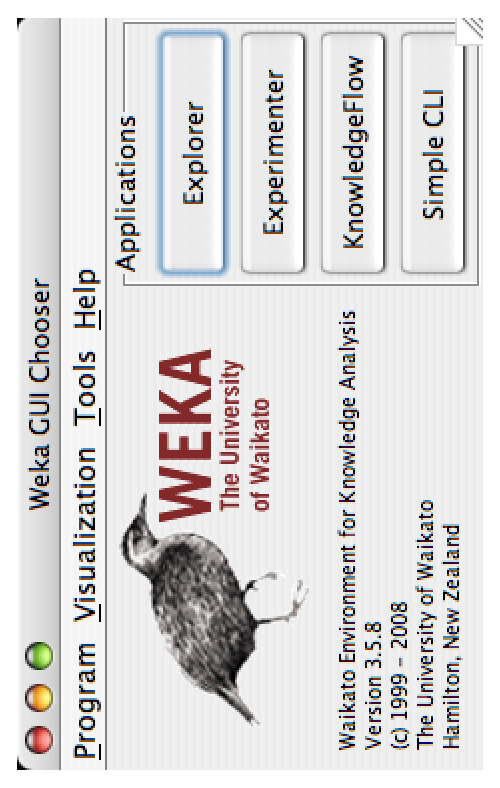
\includegraphics[angle=270,width=5cm]{images/launching/GUIChooser.eps}
\end{center}

The buttons can be used to start the following applications:

		\begin{itemize}
			\item \textbf{Explorer} An environment for exploring data with
WEKA (the rest of this documentation deals with this application in more detail).
			\item \textbf{Experimenter} An environment for performing experiments and conducting statistical tests
between learning schemes.
			\item \textbf{KnowledgeFlow} This environment supports essentially
the same functions as the Explorer but with a drag-and-drop
interface. One advantage is that it supports incremental learning.
			\item \textbf{SimpleCLI} Provides a simple command-line interface
that allows direct execution of WEKA commands for operating systems
that do not provide their own command line interface.
		\end{itemize}




The menu consists of four sections:

\begin{enumerate}
	\item \textbf{Program} \\
	        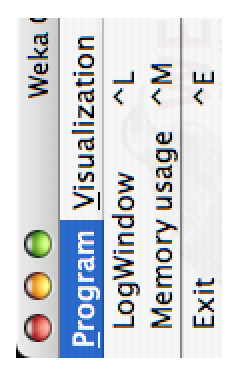
\includegraphics[angle=270,width=2cm]{images/launching/guic_program.eps}
		\begin{itemize}
			\item \textbf{LogWindow} Opens a log window that captures all that is printed to \textit{stdout} or \textit{stderr}. Useful for environments like MS Windows, where WEKA is normally not started from a terminal.
			\item \textbf{Exit} Closes WEKA.
		\end{itemize}
				
	\item \textbf{Tools} Other useful applications. \\
                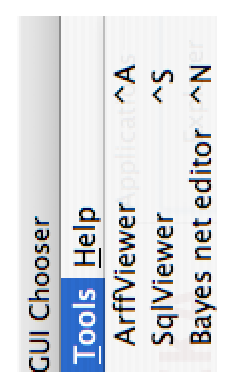
\includegraphics[angle=270,width=2cm]{images/launching/guic_tools.eps}
		\begin{itemize}
			\item \textbf{ArffViewer} An MDI application for viewing ARFF files in spreadsheet format.
			\item \textbf{SqlViewer} Represents an SQL worksheet, for querying databases via JDBC.
                        \item \textbf{Bayes net editor} An application for editing, visualizing and learning Bayes nets.
		\end{itemize}
		
	\item \textbf{Visualization} Ways of visualizing data with WEKA. \\
		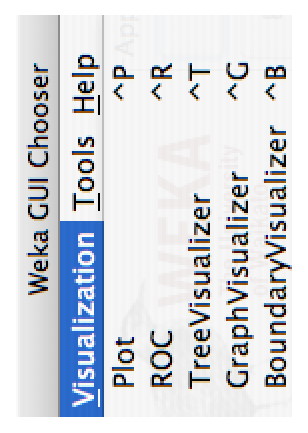
\includegraphics[angle=270,width=2cm]{images/launching/guic_visualization.eps}
		\begin{itemize}
			\item \textbf{Plot} For plotting a 2D plot of a dataset.
			\item \textbf{ROC} Displays a previously saved ROC curve.
			\item \textbf{TreeVisualizer} For displaying directed graphs, e.g., a decision tree.
			\item \textbf{GraphVisualizer} Visualizes XML BIF or DOT format graphs, e.g., for Bayesian networks.
			\item \textbf{BoundaryVisualizer} Allows the visualization of classifier decision boundaries in two dimensions.
		\end{itemize}
		
		
	\item \textbf{Help} Online resources for WEKA can be found here. \\
	        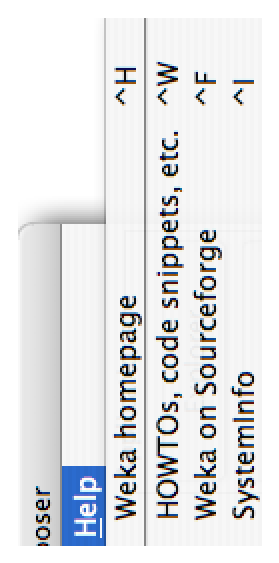
\includegraphics[angle=270,width=2cm]{images/launching/guic_help.eps}
		\begin{itemize}
			\item \textbf{Weka homepage} Opens a browser window with WEKA's homepage.
			\item \textbf{HOWTOs, code snippets, etc.} The general WekaWiki \cite{wekawiki}, containing lots of examples and HOWTOs around the development and use of WEKA.
			\item \textbf{Weka on Sourceforge} WEKA's project homepage on Sourceforge.net.
			\item \textbf{SystemInfo} Lists some internals about the Java/WEKA environment, e.g., the \texttt{CLASSPATH}.
		\end{itemize}
\end{enumerate}

To make it easy for the user to add new functionality to the menu without having to modify 
the code of WEKA itself, the GUI now offers a plugin mechanism for such add-ons. 
Due to the inherent dynamic
class discovery, plugins only need to implement the \texttt{weka.gui.MainMenuExtension}
interface and WEKA notified of the package they reside in to be displayed in the menu under 
``Extensions'' (this extra menu appears automatically as soon as extensions are discovered). 
More details can be found in the Wiki article ``Extensions for Weka's main GUI'' 
\cite{mainextensions}.

If you launch WEKA from a terminal window, some text begins scrolling in the
terminal. Ignore this text unless something goes wrong, in which case it can
help in tracking down the cause (the \textit{LogWindow} from the \textit{Program} menu 
displays that information as well).

This User Manual focuses on using the Explorer but does not explain
the individual data preprocessing tools and learning algorithms in
WEKA. For more information on the various filters and learning methods
in WEKA, see the book {\em Data Mining} \cite{witten}.


\chapter{Simple CLI}
%
%    This program is free software; you can redistribute it and/or modify
%    it under the terms of the GNU General Public License as published by
%    the Free Software Foundation; either version 2 of the License, or
%    (at your option) any later version.
%
%    This program is distributed in the hope that it will be useful,
%    but WITHOUT ANY WARRANTY; without even the implied warranty of
%    MERCHANTABILITY or FITNESS FOR A PARTICULAR PURPOSE.  See the
%    GNU General Public License for more details.
%
%    You should have received a copy of the GNU General Public License
%    along with this program; if not, write to the Free Software
%    Foundation, Inc., 675 Mass Ave, Cambridge, MA 02139, USA.
%

% Version: $Revision$

The Simple CLI provides full access to all Weka classes, i.e., classifiers, filters, clusterers, etc., but without the hassle of the CLASSPATH (it facilitates the one, with which Weka was started).

It offers a simple \textit{Weka shell} with separated commandline and output.

\begin{center}
	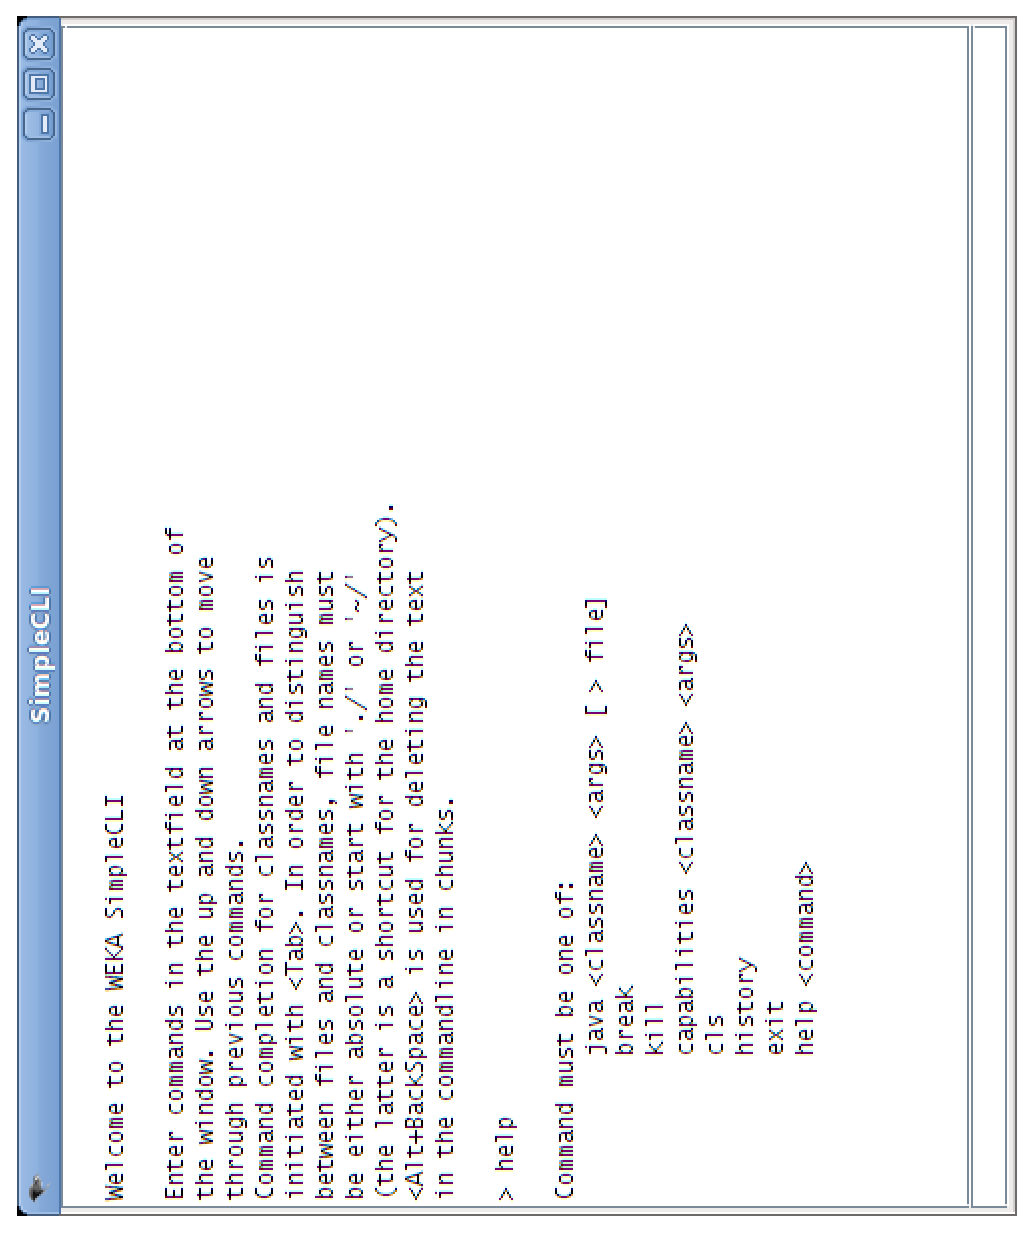
\epsfig{file=images/simplecli/simplecli_main.eps,height=10cm,angle=-90}
\end{center}


\section{Commands}
The following commands are available in the Simple CLI:
\begin{itemize}
	\item \texttt{java <classname> [<args>]} \\
		invokes a java class with the given arguments (if any)
	\item \texttt{break} \\
		stops the current thread, e.g., a running classifier, in a friendly manner
	\item \texttt{kill} \\
		stops the current thread in an unfriendly fashion
	\item \texttt{cls} \\
		clears the output area
	\item \texttt{capabilities <classname> [<args>]} \\
		lists the capabilities of the specified class, e.g., for a classifier
		with its options:
		{\small \begin{verbatim}
 		capabilities weka.classifiers.meta.Bagging -W weka.classifiers.trees.Id3
		\end{verbatim}}
	\item \texttt{exit} \\
		exits the Simple CLI
	\item \texttt{help [<command>]} \\
		provides an overview of the available commands if without a command name as argument, otherwise more help on the specified command
\end{itemize}


\section{Invocation}
In order to invoke a Weka class, one has only to prefix the class with "java". This command tells the Simple CLI to load a class and execute it with any given parameters. E.g., the J48 classifier can be invoked on the iris dataset with the following command:
\begin{verbatim}
	java weka.classifiers.trees.J48 -t c:/temp/iris.arff
\end{verbatim}

This results in the following output: 
\begin{center}
	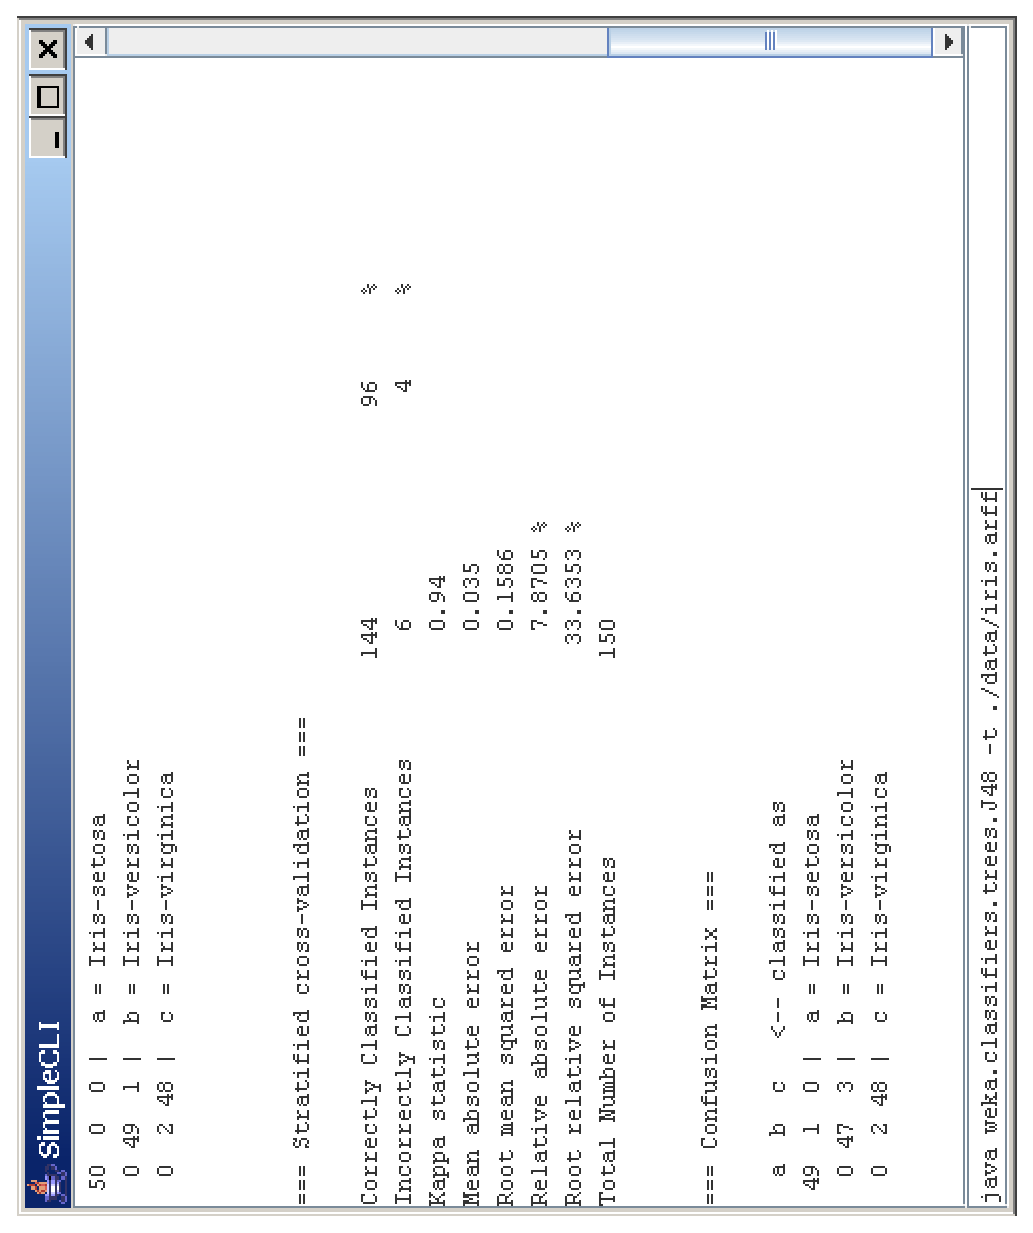
\epsfig{file=images/simplecli/simplecli_j48.eps,height=7cm,angle=-90}
\end{center}


\section{Command redirection}
Starting with this version of Weka one can perform a basic redirection:

\begin{verbatim}
	java weka.classifiers.trees.J48 -t test.arff > j48.txt
\end{verbatim}

\noindent \textbf{Note:} the \texttt{>} must be preceded and followed by a space, otherwise it is not recognized as redirection, but part of another parameter.

\section{Command completion}
Commands starting with java support completion for classnames and filenames via Tab (\texttt{Alt+BackSpace} deletes parts of the command again). In case that there are several matches, Weka lists all possible matches.

\begin{itemize}
	\item \textbf{package name completion}
		\begin{verbatim}
			java weka.cl<Tab>
		\end{verbatim}
		results in the following output of possible matches of package names:
		\begin{verbatim}
			Possible matches:
			  weka.classifiers
			  weka.clusterers
		\end{verbatim}
	\item \textbf{classname completion}
		\begin{verbatim}
			java weka.classifiers.meta.A<Tab>
		\end{verbatim}
		lists the following classes
		\begin{verbatim}
		Possible matches:
		  weka.classifiers.meta.AdaBoostM1
		  weka.classifiers.meta.AdditiveRegression
		  weka.classifiers.meta.AttributeSelectedClassifier
		\end{verbatim}
	\item \textbf{filename completion} \\
	      In order for Weka to determine whether a the string under the cursor is a classname or a filename, filenames need to be absolute (Unix/Linx: \texttt{/some/path/file}; Windows: C:$\backslash$Some$\backslash$Path$\backslash$file) or relative and starting with a dot (Unix/Linux: \texttt{./some/other/path/file}; Windows: .$\backslash$Some$\backslash$Other$\backslash$Path$\backslash$file).
\end{itemize}



\chapter{Explorer}
\input{explorer}

\chapter{Experimenter}
\input{experimenter}

\chapter{KnowledgeFlow}
%
%   This program is free software: you can redistribute it and/or modify
%   it under the terms of the GNU General Public License as published by
%   the Free Software Foundation, either version 3 of the License, or
%   (at your option) any later version.
%
%   This program is distributed in the hope that it will be useful,
%   but WITHOUT ANY WARRANTY; without even the implied warranty of
%   MERCHANTABILITY or FITNESS FOR A PARTICULAR PURPOSE.  See the
%   GNU General Public License for more details.
%
%   You should have received a copy of the GNU General Public License
%   along with this program.  If not, see <http://www.gnu.org/licenses/>.
%

% Version: $Revision$

%%%%%%%%%%%%%%%%
% Introduction %
%%%%%%%%%%%%%%%%

\section{Introduction}

The KnowledgeFlow provides an alternative to the Explorer as a
graphical front end to WEKA's core algorithms. Weka 3.8.0 and 3.9.0
contain a new implementation of the KnowledgeFlow - this new
implementation is more efficient, has a simpler API than the old
version, and now lives in the \verb+weka.knowledgeflow+ and
\verb+weka.gui.knowledgeflow+ packages. The old Knowledge Flow
implementation is still available in the \verb+weka.gui.beans+
package.

\begin{center}
  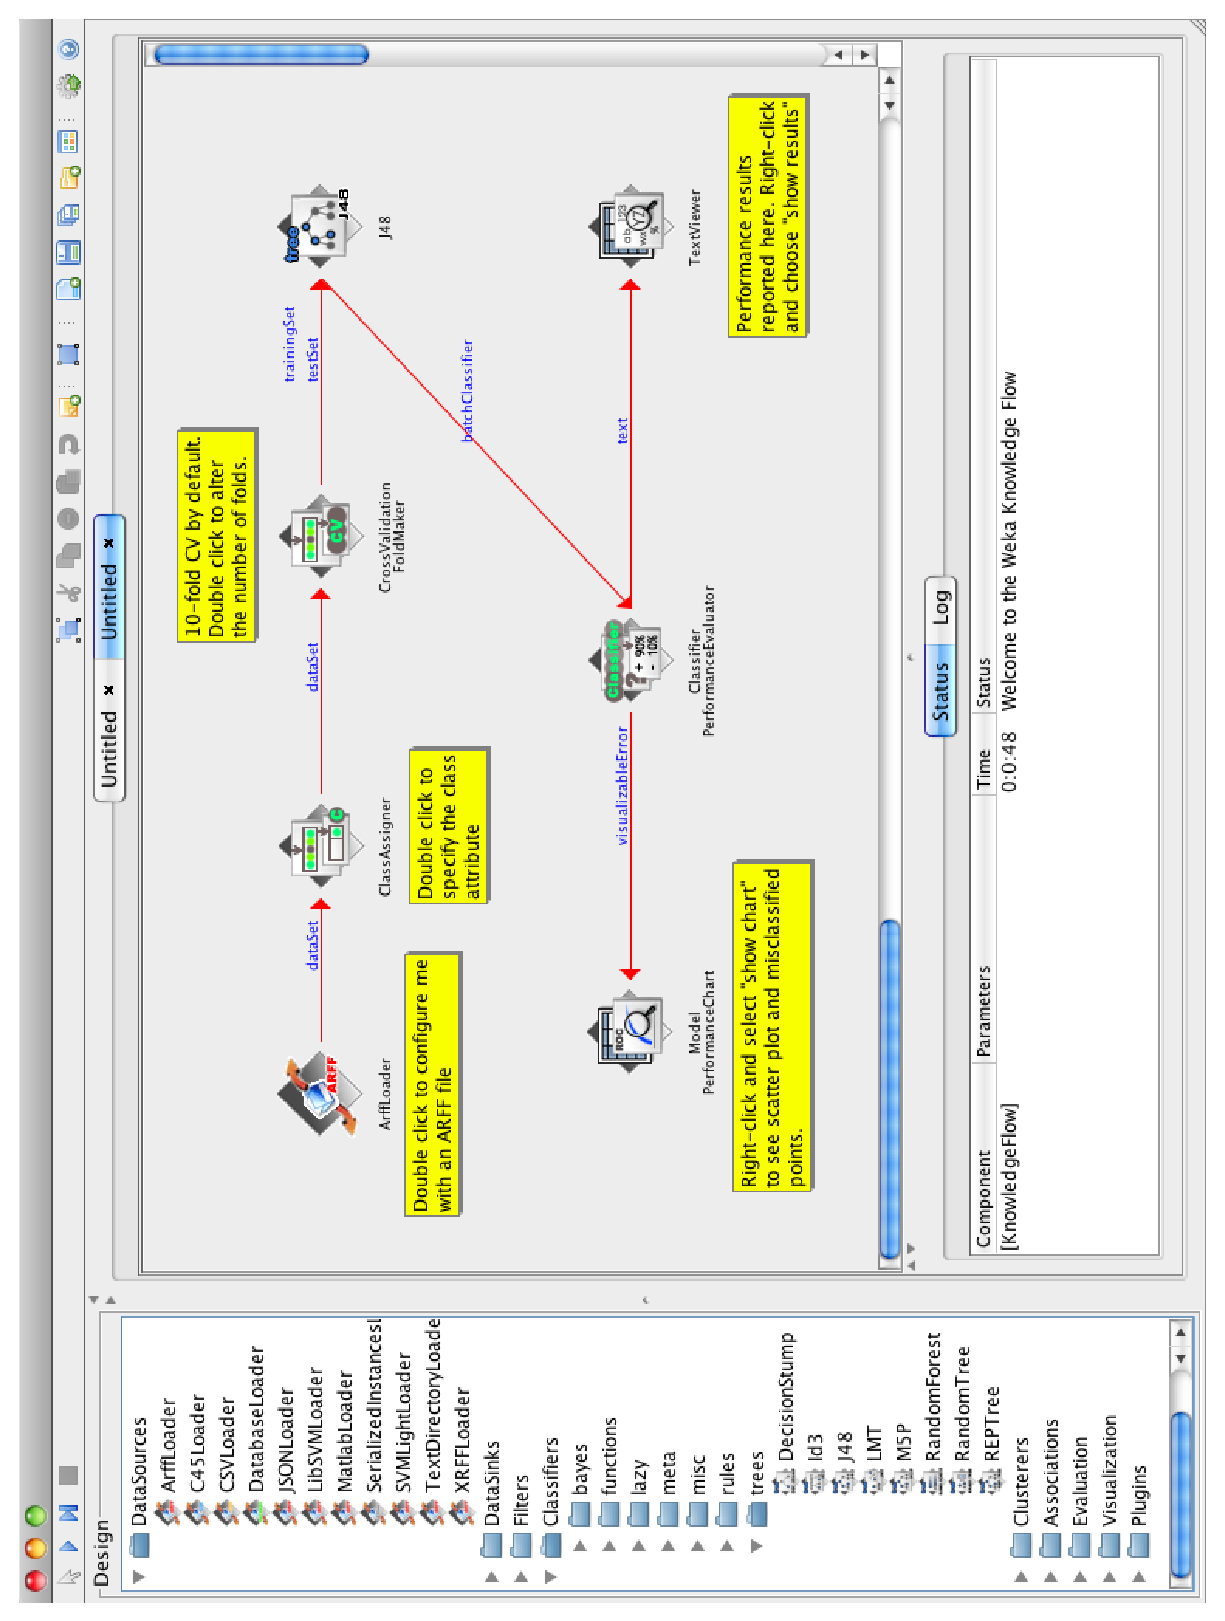
\includegraphics[width=10cm]{images/knowledgeflow/knowledgeflow.eps}
\end{center}

The KnowledgeFlow presents a \textit{data-flow} inspired interface to
WEKA. The user can select WEKA steps from a palette, place them
on a layout canvas and connect them together in order to form a
\textit{knowledge flow} for processing and analyzing data. At present,
all of WEKA's classifiers, filters, clusterers, associators, loaders
and savers are available in the KnowledgeFlow along with some extra
tools.

The KnowledgeFlow can handle data either incrementally or in batches
(the Explorer handles batch data only). Of course learning from data
incrementally requires a classifier that can be updated on an instance
by instance basis. Currently in WEKA there are ten classifiers that
can handle data incrementally:
\begin{tight_itemize}
	\item AODE
	\item IB1
	\item IBk
	\item KStar
	\item NaiveBayesMultinomialUpdateable
	\item NaiveBayesUpdateable
	\item NNge
	\item Winnow
        \item SGD
        \item SPegasos
\end{tight_itemize}

\noindent A further two classifiers are meta classifiers:
\begin{tight_itemize}
	\item \textit{RacedIncrementalLogitBoost} - that can use of any regression base
learner to learn from discrete class data incrementally.
	\item \textit{LWL} - locally weighted learning.
\end{tight_itemize}

Furthermore, other incremental streaming classifiers from the MOA
project are accessible through the ``massiveOnlineAnalysis'' package
(available for installation via the package manager).

%%%%%%%%%%%%
% Features %
%%%%%%%%%%%%

\newpage
\section{Features}

The KnowledgeFlow offers the following features:
\begin{itemize}
	\item intuitive data flow style layout
	\item process data in batches or incrementally 
	\item launch multiple start points in parallel
        \item launch multiple start points sequentially in a user-defined order
        \item fully multi-threaded - each step in a flow executes in its own thread (except for those processing streaming data)
        \item single threaded execution for streaming flows
	\item chain filters together
	\item view models produced by classifiers for each fold in a cross validation
	\item visualize performance of incremental classifiers during 
  	processing (scrolling plots of classification accuracy, RMS error, 
  	predictions etc.)
        \item plugin ``perspectives'' that add major new functionality (e.g. 3D data visualization, 
          time series forecasting environment etc.)
\end{itemize}

\newpage
\section{Flow Steps}
Steps available in the KnowledgeFlow:

\subsection{DataSources} All of WEKA's loaders are available.
%\begin{center}
	%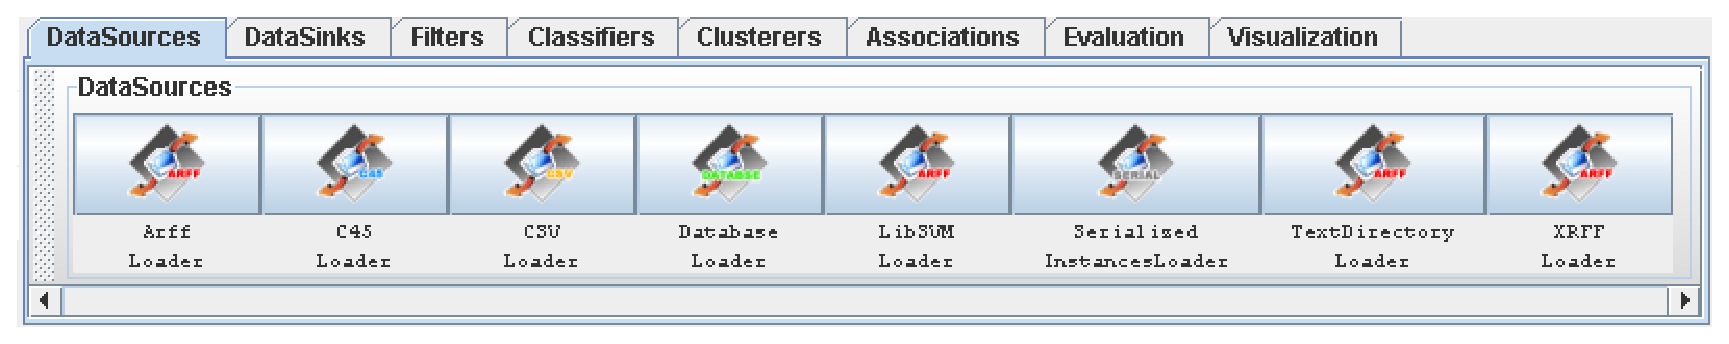
\epsfig{file=images/knowledgeflow/components_datasources.eps,height=2cm}
%\end{center}

\subsection{DataSinks} All of WEKA's savers are available. Along with the
following KnowledgeFlow-specific ones:

\begin{itemize}  
\item \textit{TextSaver} - save text carried by a text connection out to a file.
\item \textit{ImageSaver} - save the image data carried by an image connection
out to a file in either PNG or GIF format.
\item \textit{SerializedModelSaver} - save the classifier or clusterer
  encapsulated in a batchClassifier, incrementalClassifier or batchClusterer
  connection out to a file.
\end{itemize}

\subsection{DataGenerators} All of WEKA's data generators are available.

%\begin{center}
%	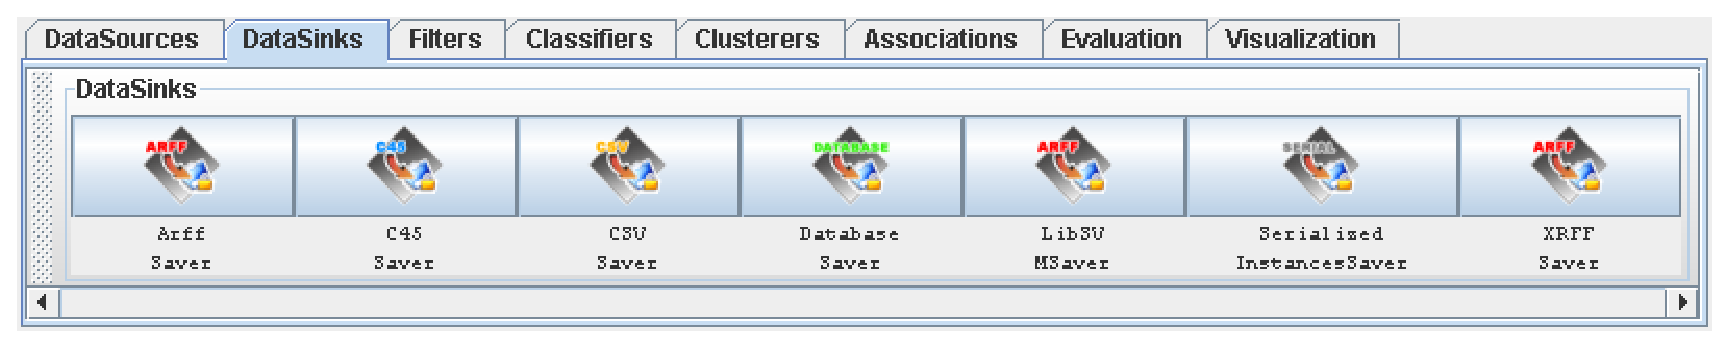
\epsfig{file=images/knowledgeflow/components_datasinks.eps,height=2cm}
%\end{center}

\subsection{Filters} All of WEKA's filters are available.
%\begin{center}
%	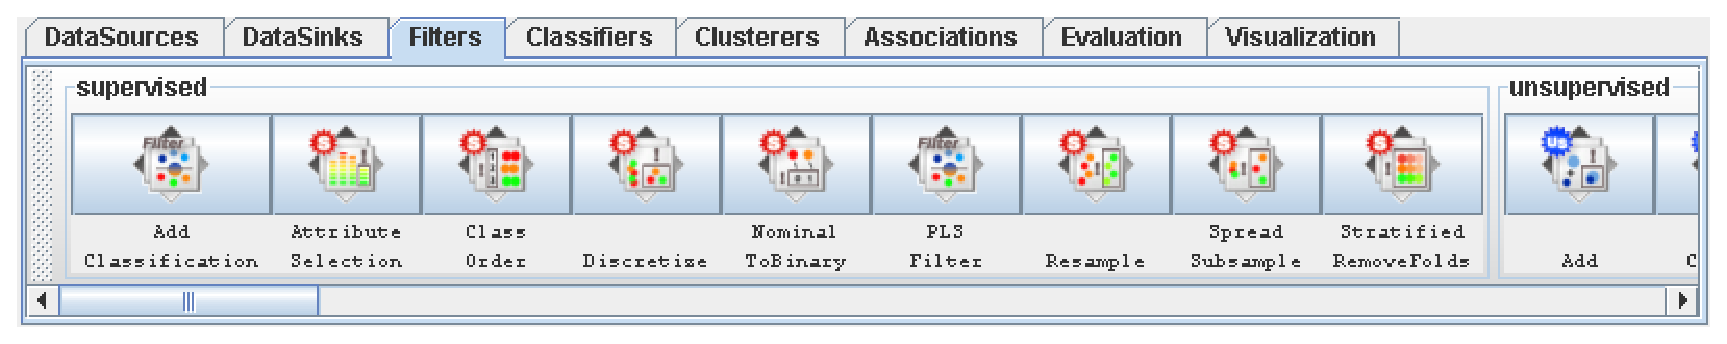
\epsfig{file=images/knowledgeflow/components_filters.eps,height=2cm}
%\end{center}

\subsection{Classifiers} All of WEKA's classifiers are available.
%\begin{center}
%	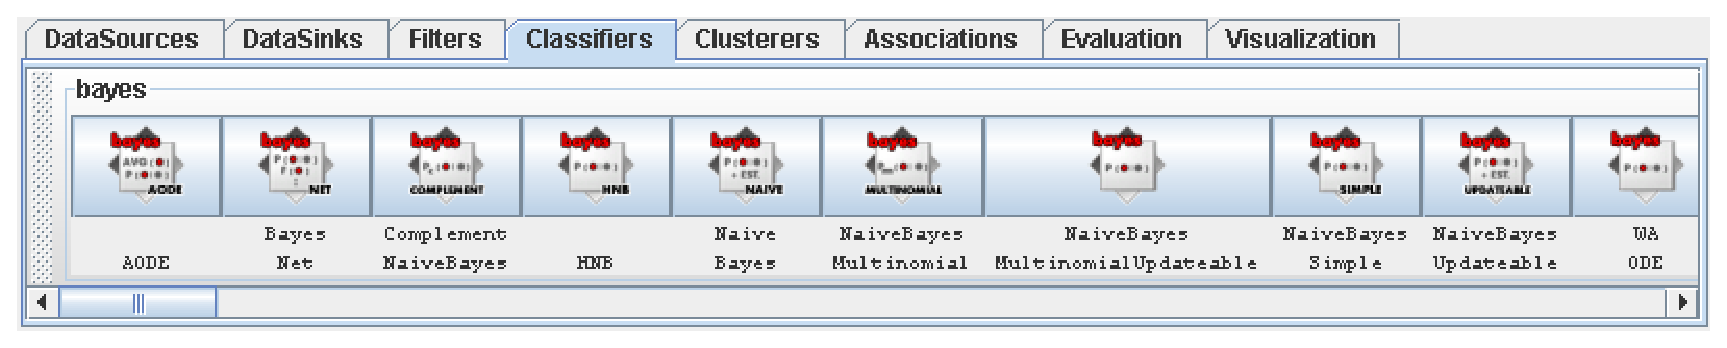
\epsfig{file=images/knowledgeflow/components_classifiers.eps,height=2cm}
%\end{center}

\subsection{Clusterers} All of WEKA's clusterers are available.
%\begin{center}
%	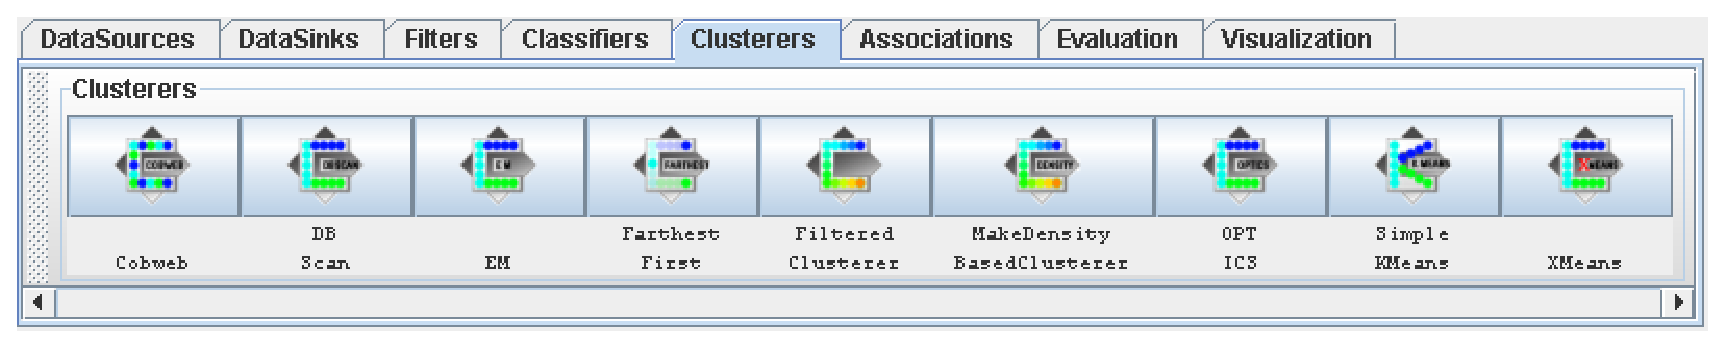
\epsfig{file=images/knowledgeflow/components_clusterers.eps,height=2cm}
%\end{center}

\subsection{Attribute selection} All of WEKA's attribute and subset evaluators
are available, along with all of the search methods.

\subsection{Evaluation}
%\begin{center}
%	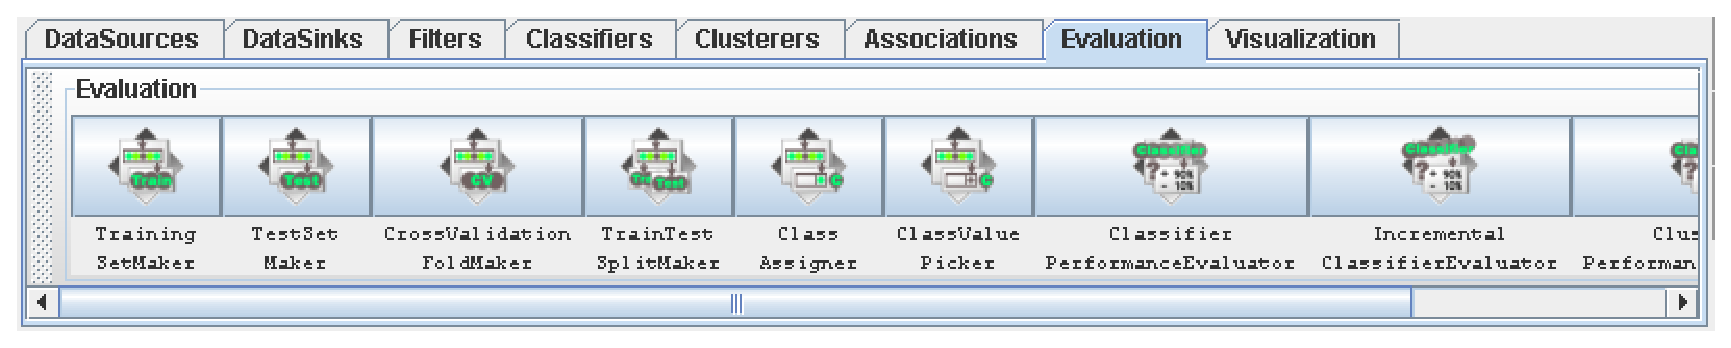
\epsfig{file=images/knowledgeflow/components_evaluation.eps,height=2cm}
%\end{center}

\begin{itemize}
	\item \textit{TrainingSetMaker} - make a data set into a training set.
	\item \textit{TestSetMaker} - make a data set into a test set.
	\item \textit{CrossValidationFoldMaker} - split any data set, training 
	set or test set into folds.
	\item \textit{TrainTestSplitMaker} - split any data set, training set 
	or test set into a training set and a test set.
        \item \textit{InstanceStreamToBatchMaker} - collects the instances in
          an incoming instance stream and outputs them as a batch set of Instances.
	\item \textit{ClassAssigner} - assign a column to be the class for any 
	data set, training set or test set.
	\item \textit{ClassValuePicker} - choose a class value to be considered 
	as the ``positive'' class. This is useful when generating data for ROC style 
	curves (see \textit{ModelPerformanceChart} below and example \ref{exampleroc}).
	\item \textit{ClassifierPerformanceEvaluator} - evaluate the performance of 
	batch trained/tested classifiers.
	\item \textit{IncrementalClassifierEvaluator} - evaluate the performance of 
	incrementally trained classifiers.
	\item \textit{ClustererPerformanceEvaluator} - evaluate the performance of 
	batch trained/tested clusterers.
	\item \textit{PredictionAppender} - append classifier predictions to a test 
	set. For discrete class problems, can either append predicted class labels or
	probability distributions.
\end{itemize}

\subsection{Visualization}
%\begin{center}
%	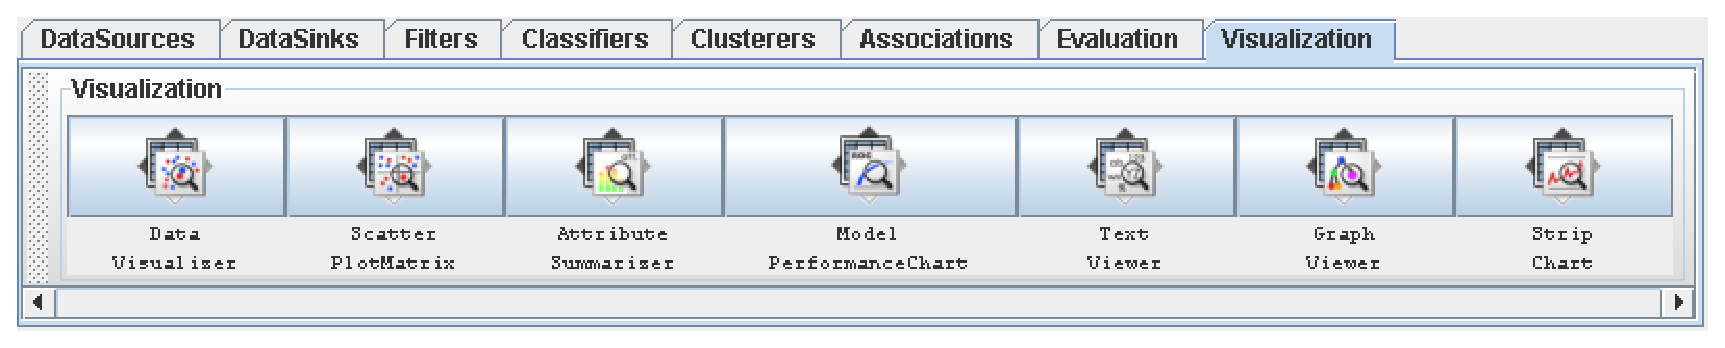
\epsfig{file=images/knowledgeflow/components_visualization.eps,height=2cm}
%\end{center}

\begin{itemize}
	\item \textit{DataVisualizer} - a step that can pop up a panel for 
	visualizing data in a single large 2D scatter plot.
	\item \textit{ScatterPlotMatrix} - a step that can pop up a panel 
	containing a matrix of small scatter plots (clicking on a small plot 
	pops up a large scatter plot).
	\item \textit{AttributeSummarizer} - a step that can pop up a panel 
	containing a matrix of histogram plots - one for each of the attributes 
	in the input data.
	\item \textit{ModelPerformanceChart} - a step that can pop up a 
	panel for visualizing threshold (i.e. ROC style) curves.
        \item \textit{CostBenefitAnalysis} - a step that can popup a graphical
          tool for exploring cost/benefit tradeoffs by interactively selecting
          different population sizes from a ranked list of prospects or by 
          varying the threshold on the predicted probability of the positive class. It
          displays both a cumulative gains chart and a cost/benefit plot.
	\item \textit{TextViewer} - a step for showing textual data. Can show 
	data sets, classification performance statistics etc.
	\item \textit{GraphViewer} - a step that can pop up a panel for 
	visualizing tree based models.
	\item \textit{StripChart} - a step that can pop up a panel that displays 
	a scrolling plot of data (used for viewing the online performance of 
	incremental classifiers).
        \item \textit{ImageViewer} - a step that can popup a visualization for static
          image data.
        \item \textit{BoundaryPlotter} - a step that accepts a dataSet, along with one
          or more info connections from classifiers or clusterers to execute, and generates
          prediction boundary plots. The resulting plots can be viewed in a popup visualization.
\end{itemize}

\subsection{Flow}

\begin{itemize}
  \item \textit{SetVariables} - set the values of variables used in the flow. This is useful for
    testing flows that use variables before they are executed in an environment where the variables
    will have meaningful values. This step does not need to be connected to any others - just place
    one on the layout.
  \item \textit{MakeResourceIntensive} - a step that alters which executor service is used to
    execute the step immediately downstream. By default, most steps execute in the main executor
    service. However, there is a secondary executor service, using a limited number of threads, 
    available for executing high resource (cpu/memory) tasks and steps. The Classifier step 
    executes in the high resource executor by default because it could potentially process
    many cross-validation folds - this way it won't starve other steps of CPU or memory
    resources. The \textit{MakeResourceIntensive} can be used to force a step to use a particular
    executor service.
  \item \textit{Block} - a step that blocks incoming connections until a specified step in the flow
    has finished executing.
  \item \textit{Appender} - appends incoming batches or streams of data into one batch/stream. All
    inputs must be of the same type (i.e. all batch or all stream). An amalgamated output is created
    that is a combination of all the incoming attributes.
  \item \textit{FlowByExpression} - a step that splits incoming instances (or instance streams) 
    according to the evaluation of a logical expression. The expression can test the values of
    one or more incoming attributes. The test can involve constants or comparing the value of
    one attribute's values to another.
  \item \textit{InstanceStreamToBatchMaker} - converts an incoming instance stream to a batch
    (i.e. accepts an instance connection and outputs a dataSet connection).
  \item \textit{Join} - a step that performs an inner join on two incoming dataSet or instance
    stream connections. \textbf{Important}: assumes that both inputs are sorted in ascending order
    of the key fields. A \textit{Sorter} step can be used to sort data before it is input to \textit{Join}.

\end{itemize}

\subsection{Tools}

\begin{itemize}
   \item \textit{Sorter} - a step that sorts incoming instances in ascending or descending order
     according to the values of user-specified attributes. Instances can be sorted according to
     multiple attributes (defined in order). Handles datasets larger than can be fit into main
     memory via instance connections and specifying the in-memory buffer size. Implements a 
     merge sort by writing the sorted in-memory buffer to a file when full, and then interleaving
     instances from the disk-based file(s) when the incoming stream has finished.
   \item \textit{SubstringReplacer} - replaces substrings in \textit{String} attributes using either
     a literal match-and-replace, or regular expression matching.
   \item \textit{SubstringLabeler} - a step that labels instances according to substring or regular
     expression matches in \textit{String} attributes. The user can specify the attributes to match
     against and associated label to create by defining ``match'' rules. A new attribute is appended
     to the data to contain the label. Rules are applied in order when processing instances, and the
     label associated with the first matching rule is applied. Non-matching instances can either receive
     a missing value for the label attribute or be ``consumed'' (i.e. they are not output).
\end{itemize}

%%%%%%%%%%%%
% Examples %
%%%%%%%%%%%%

\newpage
\section{Examples}

%%%%%%%%%%%%%%%%%%%%%%%%%%%%%%%%
% Example: cross-validated J48 %
%%%%%%%%%%%%%%%%%%%%%%%%%%%%%%%%

\subsection{Cross-validated J48}
Setting up a flow to load an ARFF file (batch mode) and
perform a cross-validation using J48 (WEKA's C4.5 implementation). This example
can be accessed from the ``Cross validation'' entry of the popup menu that
appears when the ``templates'' button in the toolbar is clicked.

\begin{center}
  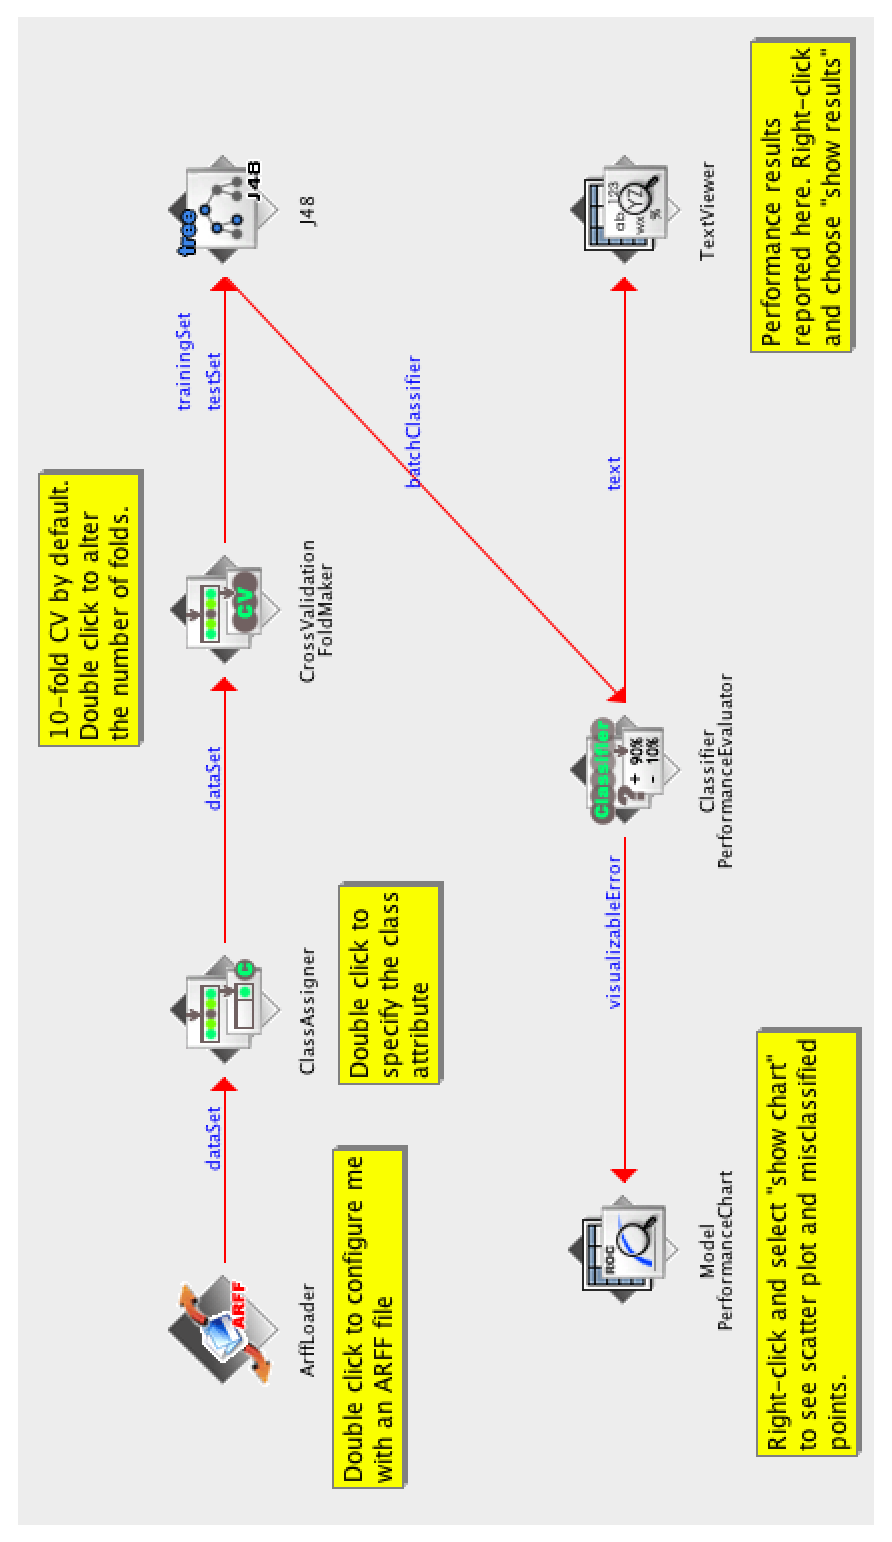
\includegraphics[angle=270,width=10cm]{images/knowledgeflow/example_j48.eps}
	%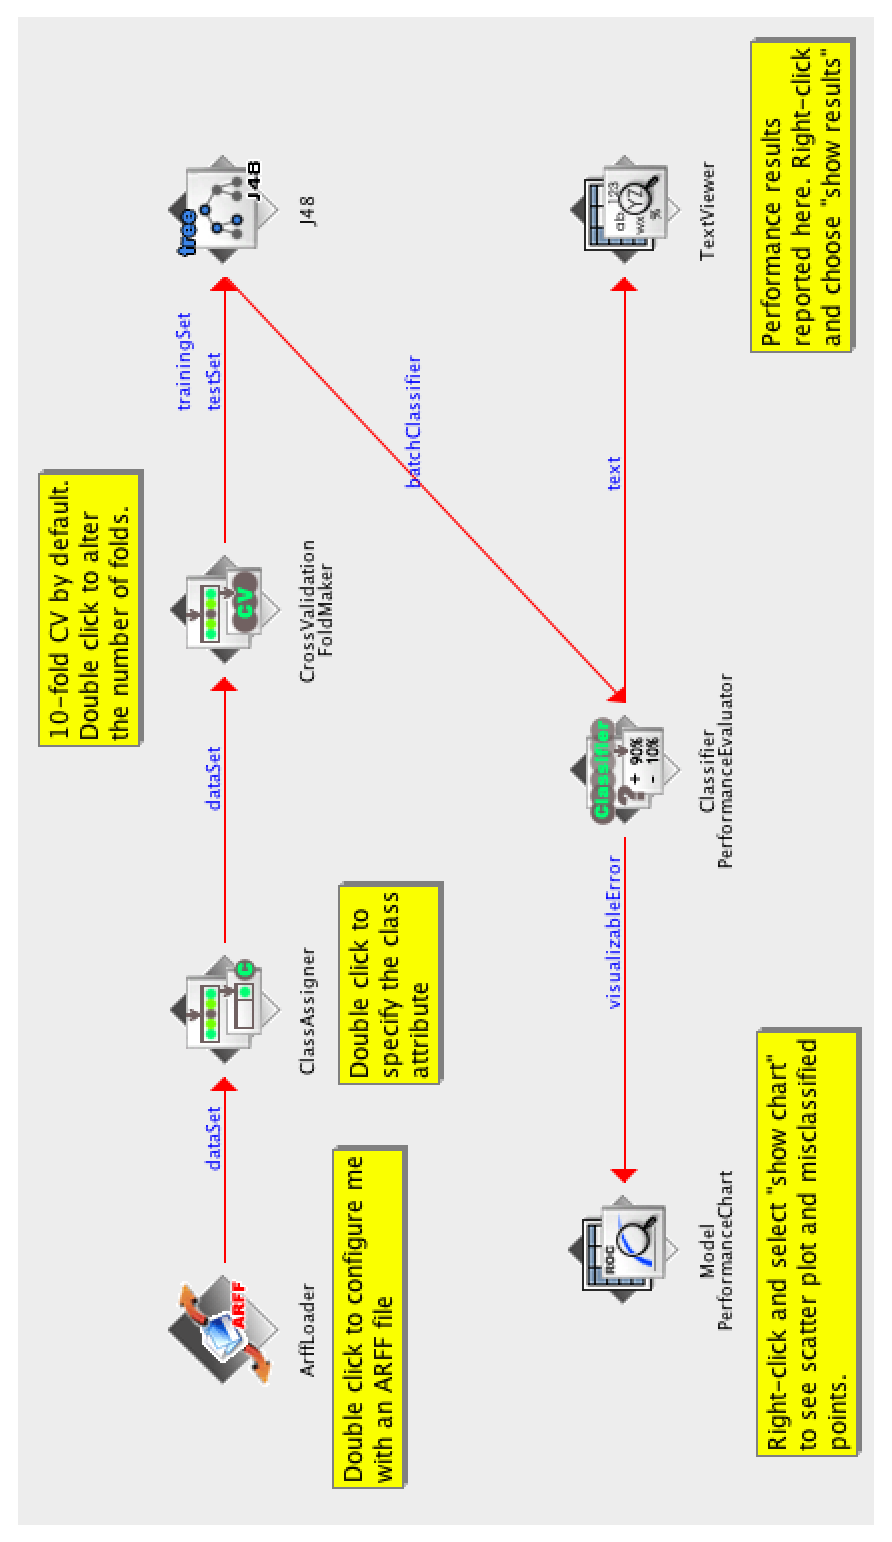
\epsfig{file=images/knowledgeflow/example_j48.eps,height=4.5cm}
\end{center}

\begin{itemize}
	\item Expand the DataSources entry in the \textit{Design} panel and
          choose \textit{ArffLoader} (the mouse pointer will change to
          a \textit{cross hairs}).

	\item Next place the ArffLoader step on the layout area by clicking
	somewhere on the layout (a copy of the ArffLoader icon will appear on
	the layout area).

	\item Next specify an ARFF file to load by first right clicking the mouse
	over the ArffLoader icon on the layout. A pop-up menu will
	appear. Select \textit{Configure} under \textit{Edit} in the list from this menu and
	browse to the location of your ARFF file.

	\item Next click expand the \textit{Evaluation} entry in the
          \textit{Design} panel and choose the \textit{ClassAssigner}
          (allows you to choose which column to be the class)
          step from the toolbar. Place this on the layout.

	\item Now connect the ArffLoader to the ClassAssigner: first right click
	over the ArffLoader and select the \textit{dataSet} under \textit{Connections} in
	the menu. A \textit{rubber band} line will appear. Move the mouse over the
	ClassAssigner step and left click - a red line labeled \textit{dataSet}
	will connect the two steps.

	\item Next right click over the ClassAssigner and choose \textit{Configure} from
	the menu. This will pop up a window from which you can specify which
	column is the class in your data (last is the default).

	\item Next grab a \textit{CrossValidationFoldMaker} step
          from the Evaluation entry in the \textit{Design} panel and
          place it on the layout. Connect the ClassAssigner to the
          CrossValidationFoldMaker by right clicking over
          \textit{ClassAssigner} and selecting \textit{dataSet} from
          under \textit{Connections} in the menu.

	\item Next expand the \textit{Classifiers} entry and then the
          \textit{trees} sub-entry in the \textit{Design} panel and
          choose the \textit{J48} step. Place a J48 step on
          the layout.

	\item Connect the CrossValidationFoldMaker to J48 TWICE by first choosing
	\textit{trainingSet} and then \textit{testSet} from the pop-up menu for the
	CrossValidationFoldMaker.

	\item Next go back to the \textit{Evaluation} entry and place
          a \textit{ClassifierPerformanceEvaluator} step on the
          layout. Connect J48 to this step by selecting the
          \textit{batchClassifier} entry from the pop-up menu for J48.

	\item Next go to the \textit{Visualization} entry and place a \textit{TextViewer}
	step on the layout. Connect the ClassifierPerformanceEvaluator to
	the TextViewer by selecting the \textit{text} entry from the pop-up menu for
	ClassifierPerformanceEvaluator.

	\item Now start the flow executing by pressing the
          \textit{play} button on the toolbar at the top of the
          window. Progress information for each step in the flow
          will appear in the \textit{Status} area and \textit{Log} at
          the bottom of the window.
\end{itemize}

When finished you can view the results by choosing \textit{Show results} from
the pop-up menu for the \textit{TextViewer} step.

Other cool things to add to this flow: connect a \textit{TextViewer} and/or a
\textit{GraphViewer} to J48 in order to view the textual or graphical
representations of the trees produced for each fold of the cross
validation (this is something that is not possible in the Explorer).

%%%%%%%%%%%%%%%%%%%%%%%%%
% Example: multiple ROC %
%%%%%%%%%%%%%%%%%%%%%%%%%

\newpage
\subsection{Plotting multiple ROC curves}
\label{exampleroc}
The KnowledgeFlow can draw multiple ROC curves in the same plot
window, something that the Explorer cannot do. In this example we use
\textit{J48} and \textit{RandomForest} as classifiers. This example
can be accessed from the ``ROC curves for two classifiers'' entry of
the popup menu that appears when the ``templates'' button in the
toolbar is clicked. It can also be found on the \textit{WekaWiki}
as well \cite{multipleroc}.

\begin{center}
  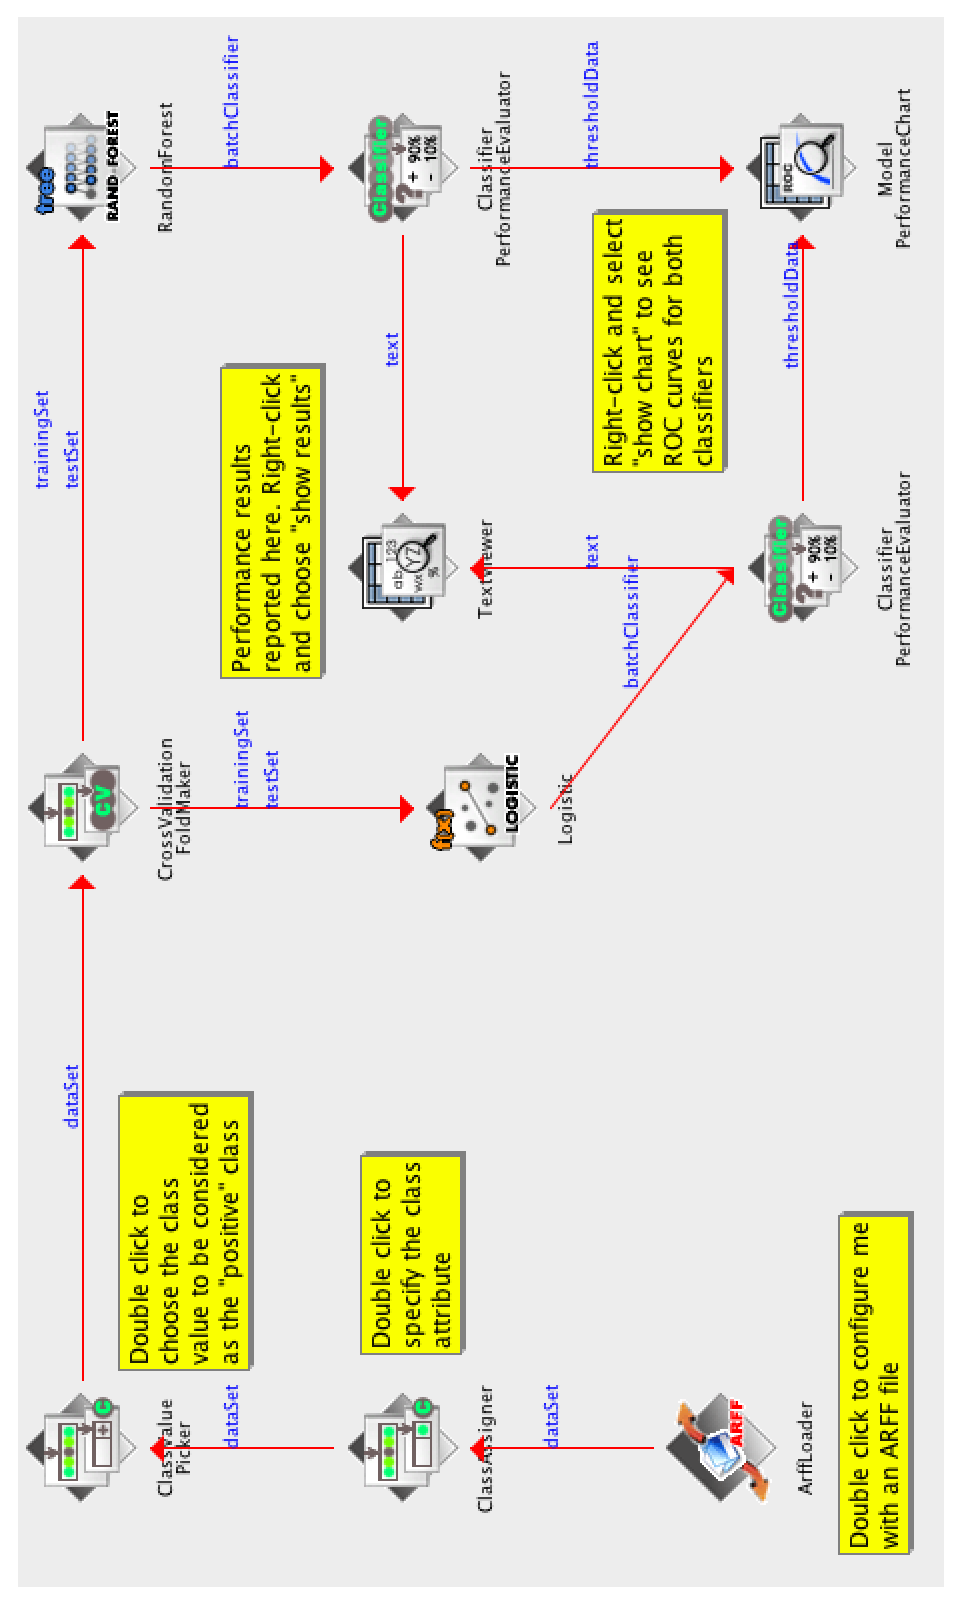
\includegraphics[angle=270,width=10cm]{images/knowledgeflow/example_multiple_roc.eps}
%	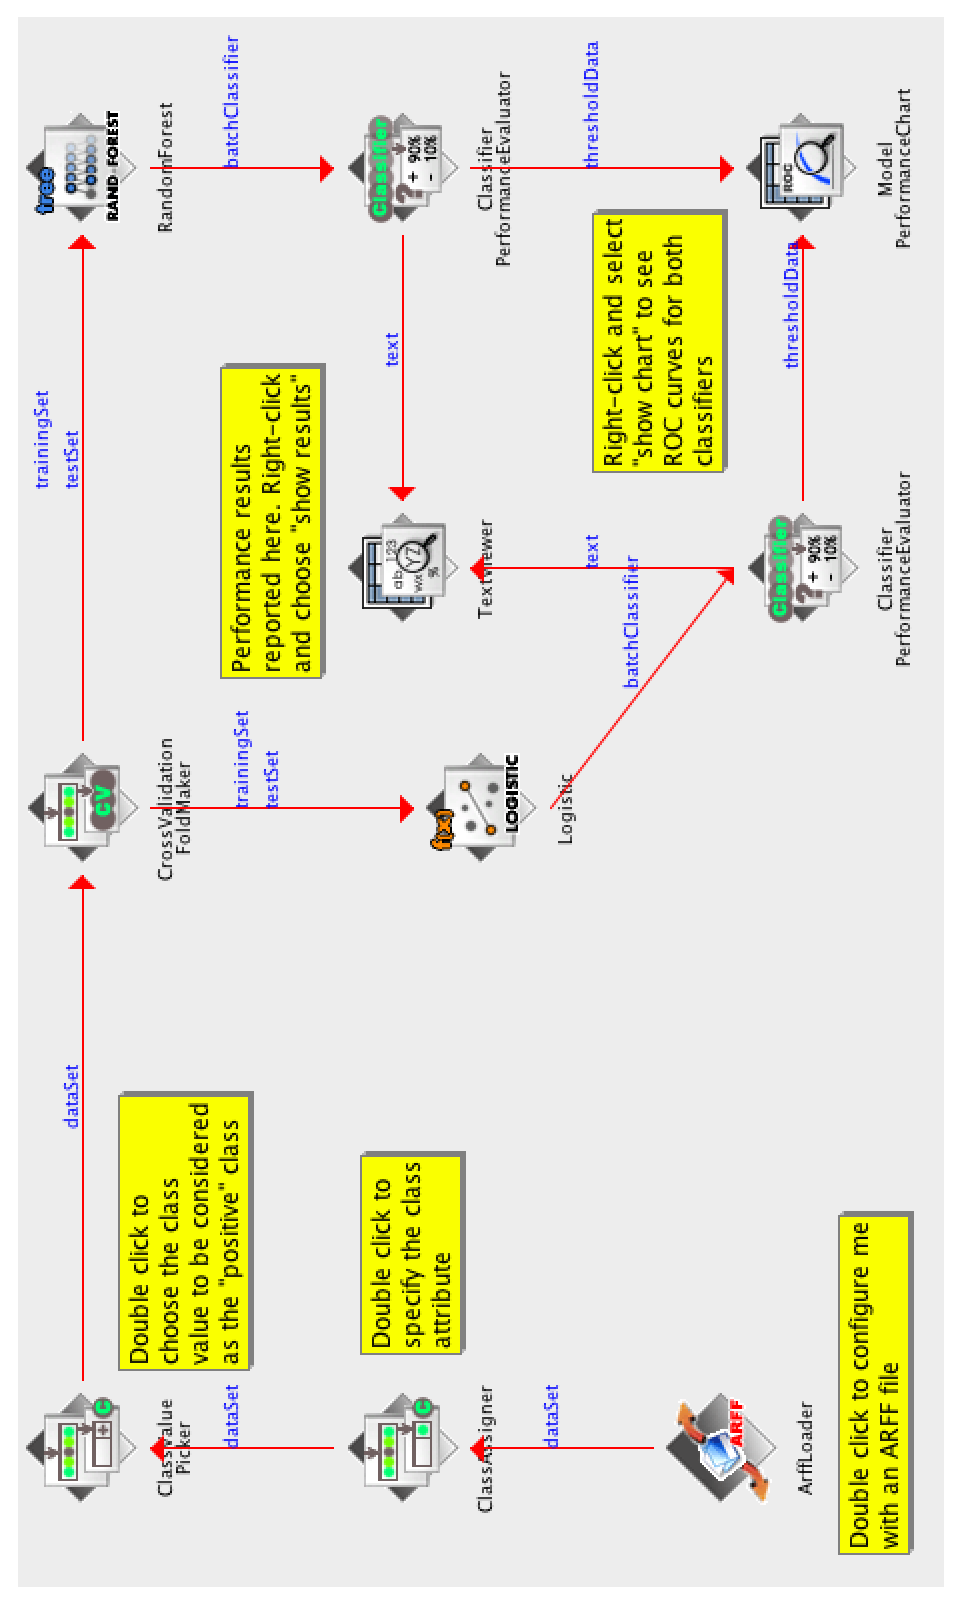
\epsfig{file=images/knowledgeflow/example_multiple_roc.eps,height=4cm}
\end{center}

\begin{itemize}
	\item Click on the DataSources entry in the \textit{Design}
          panel and choose \textit{ArffLoader} (the mouse pointer will
          change to a \textit{cross hairs}).

	\item Next place the ArffLoader step on the layout area by clicking
	somewhere on the layout (a copy of the ArffLoader icon will appear on
	the layout area).

	\item Next specify an ARFF file to load by first right clicking the mouse
	over the ArffLoader icon on the layout. A pop-up menu will
	appear. Select \textit{Configure} under \textit{Edit} in the list from this menu and
	browse to the location of your ARFF file.

	\item Next click the \textit{Evaluation} entry in the
          \textit{Design} panel and choose the \textit{ClassAssigner}
          (allows you to choose which column to be the class)
          step from the toolbar. Place this on the layout.

	\item Now connect the ArffLoader to the ClassAssigner: first right click
	over the ArffLoader and select the \textit{dataSet} under \textit{Connections} in
	the menu. A \textit{rubber band} line will appear. Move the mouse over the
	ClassAssigner step and left click - a red line labeled \textit{dataSet}
	will connect the two stepss.

	\item Next right click over the ClassAssigner and choose \textit{Configure} from
	the menu. This will pop up a window from which you can specify which
	column is the class in your data (last is the default).

	\item Next choose the \textit{ClassValuePicker} (allows you to
          choose which class label to be evaluated in the ROC)
          step from \textit{Evaluation}. Place this on
          the layout and right click over \textit{ClassAssigner} and
          select \textit{dataSet} from under \textit{Connections} in
          the menu and connect it with the \textit{ClassValuePicker}.

	\item Next grab a \textit{CrossValidationFoldMaker} step
          from \textit{Evaluation} and place it on the layout. Connect
          the ClassAssigner to the CrossValidationFoldMaker by right
          clicking over \textit{ClassAssigner} and selecting
          \textit{dataSet} from under \textit{Connections} in the
          menu.

	\item Next click on the \textit{Classifiers} entry in the
          \textit{Design} panel and choose the \textit{J48} step
          from the \textit{trees} sub-entry. Place a J48 step on
          the layout.

	\item Connect the CrossValidationFoldMaker to J48 TWICE by first choosing
	\textit{trainingSet} and then \textit{testSet} from the pop-up menu for the
	CrossValidationFoldMaker.

	\item Repeat these two steps with the RandomForest classifier.

	\item Next go back to \textit{Evaluation} and place a
	\textit{ClassifierPerformanceEvaluator} step on the layout. Connect J48
	to this step by selecting the \textit{batchClassifier} entry from the
	pop-up menu for J48. Add another \textit{ClassifierPerformanceEvaluator} for
	RandomForest and connect them via \textit{batchClassifier} as well.

	\item Next go to the \textit{Visualization} entry and place a 
	\textit{ModelPerformanceChart} step on the layout. Connect both 
	ClassifierPerformanceEvaluators to the ModelPerformanceChart by selecting 
	the \textit{thresholdData} entry from the pop-up menu for ClassifierPerformanceEvaluator.

	\item Now start the flow executing by pressing the
          \textit{play} button on the toolbar at the top of the
          window. Progress information for each step in the flow
          will appear in the \textit{Status} bar and \textit{Log} at
          the bottom of the window.
	
	\item Select \textit{Show plot} from the popup-menu of the 
	\textit{ModelPerformanceChart} under the \textit{Actions} section.
\end{itemize}

Here are the two ROC curves generated from the UCI dataset \textit{credit-g}, 
evaluated on the class label \textit{good}:

\begin{center}
	\epsfig{file=images/knowledgeflow/example_multiple_roc_output.eps,height=8.5cm}
\end{center}

%%%%%%%%%%%%%%%%%%%%%%%%%%%%%%%%%%%%%%%%%%%
% Example: processing data incrementally  %
%%%%%%%%%%%%%%%%%%%%%%%%%%%%%%%%%%%%%%%%%%%

\newpage
\subsection{Processing data incrementally}

Some classifiers, clusterers and filters in Weka can handle data
incrementally in a streaming fashion. Here is an example of training
and testing \textit{naive Bayes} incrementally. The results are sent
to a \textit{TextViewer} and predictions are plotted by a
\textit{StripChart} step. This example can be accessed from the
``Learn and evaluate naive Bayes incrementally'' entry of the popup menu that
appears when the ``templates'' button in the toolbar is clicked.

\begin{center}
  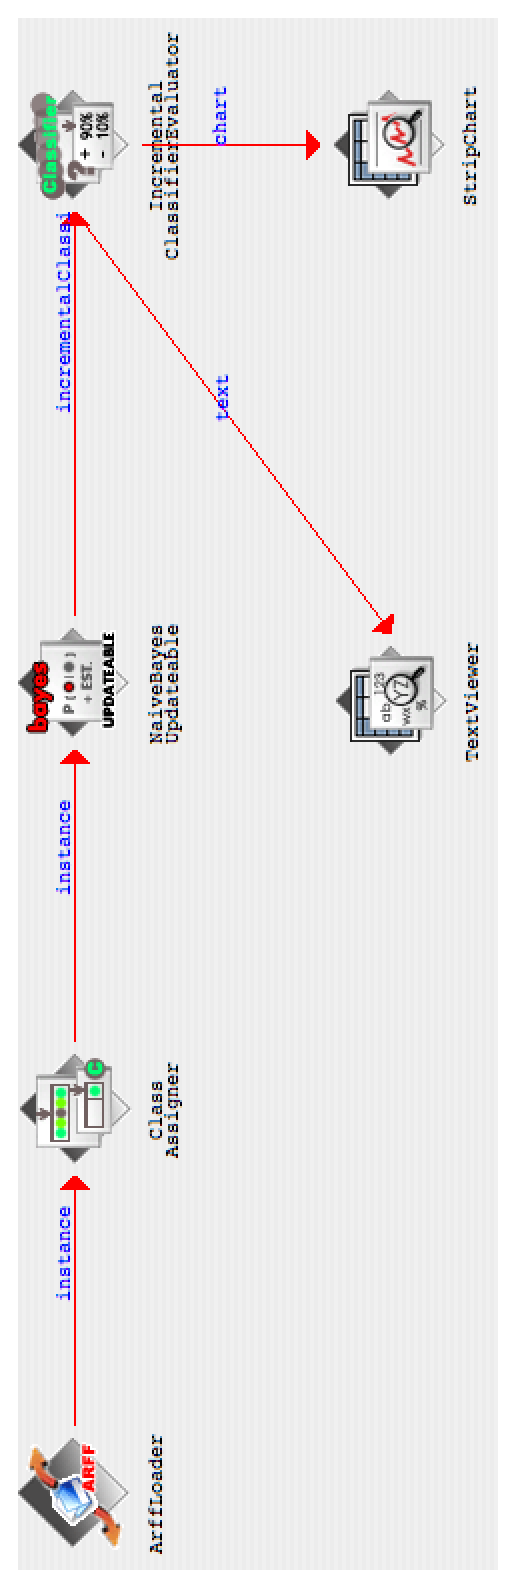
\includegraphics[angle=270,width=10cm]{images/knowledgeflow/IncrementalFlow.eps}
\end{center}

\begin{itemize}
        \item Expand the DataSources entry in the \textit{Design}
          panel and choose \textit{ArffLoader} (the mouse pointer will
          change to a \textit{cross hairs}).

	\item Next place the ArffLoader step on the layout area by clicking
	somewhere on the layout (a copy of the ArffLoader icon will appear on
	the layout area).

	\item Next specify an ARFF file to load by first right clicking the mouse
	over the ArffLoader icon on the layout. A pop-up menu will
	appear. Select \textit{Configure} under \textit{Edit} in the list from this menu and
	browse to the location of your ARFF file.

	\item Next expand the \textit{Evaluation} entry in the
          \textit{Design} panel and choose the \textit{ClassAssigner}
          (allows you to choose which column to be the class). Place
          this on the layout.

	\item Now connect the ArffLoader to the ClassAssigner: first right click
	over the ArffLoader and select the \textit{dataSet} under \textit{Connections} in
	the menu. A \textit{rubber band} line will appear. Move the mouse over the
	ClassAssigner step and left click - a red line labeled \textit{dataSet}
	will connect the two steps.

	\item Next right click over the \textit{ClassAssigner} and choose \textit{Configure} from
	the menu. This will pop up a window from which you can specify which
	column is the class in your data (last is the default).

        \item Now grab a \textit{NaiveBayesUpdateable} step from the \textit{bayes}
        section of the \textit{Classifiers} entry and place it on the layout.

        \item Next connect the \textit{ClassAssigner} to \textit{NaiveBayesUpdateable}
        using a \textit{instance} connection.

        \item Next place an \textit{IncrementalClassiferEvaluator} from the \textit{Evaluation}
        entry onto the layout and connect \textit{NaiveBayesUpdateable} to it using a
        \textit{incrementalClassifier} connection.

        \item Next place a \textit{TextViewer} step from the \textit{Visualization}
        entry on the Layout. Connect the \textit{IncrementalClassifierEvaluator} to
        it using a \textit{text} connection.

        \item Next place a \textit{StripChart} step from the \textit{Visualization}
        entry on the layout and connect \textit{IncrementalClassifierEvaluator} to it
        using a \textit{chart} connection.

        \item Display the \textit{StripChart's} chart by right-clicking over it and choosing
        \textit{Show chart} from the pop-up menu. Note: the \textit{StripChart} can be configured
        with options that control how often data points and labels are displayed.

        \item Finally, start the flow by pressing the \textit{play} button on the toolbar at the top of the window.        
\end{itemize}

\begin{center}
  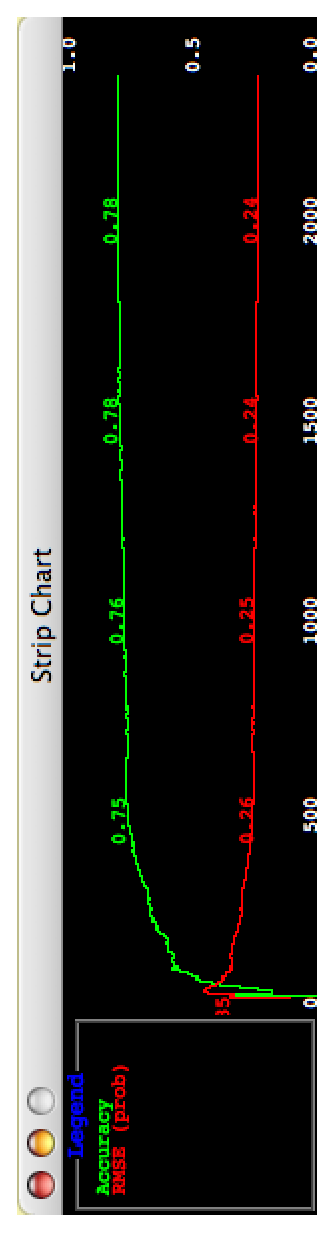
\includegraphics[angle=270,width=12cm]{images/knowledgeflow/IncrementalChart.eps}
\end{center}

Note that, in this example, a prediction is obtained from naive Bayes
for each incoming instance {\bf before} the classifier is trained
(updated) with the instance. If you have a pre-trained classifier, you
can specify that the classifier {\bf not} be updated on incoming
instances by unselecting the check box in the configuration dialog for
the classifier. If the pre-trained classifier is a {\bf batch}
classifier (i.e. it is not capable of incremental training) then you
will only be able to test it in an incremental fashion.

\begin{center}
  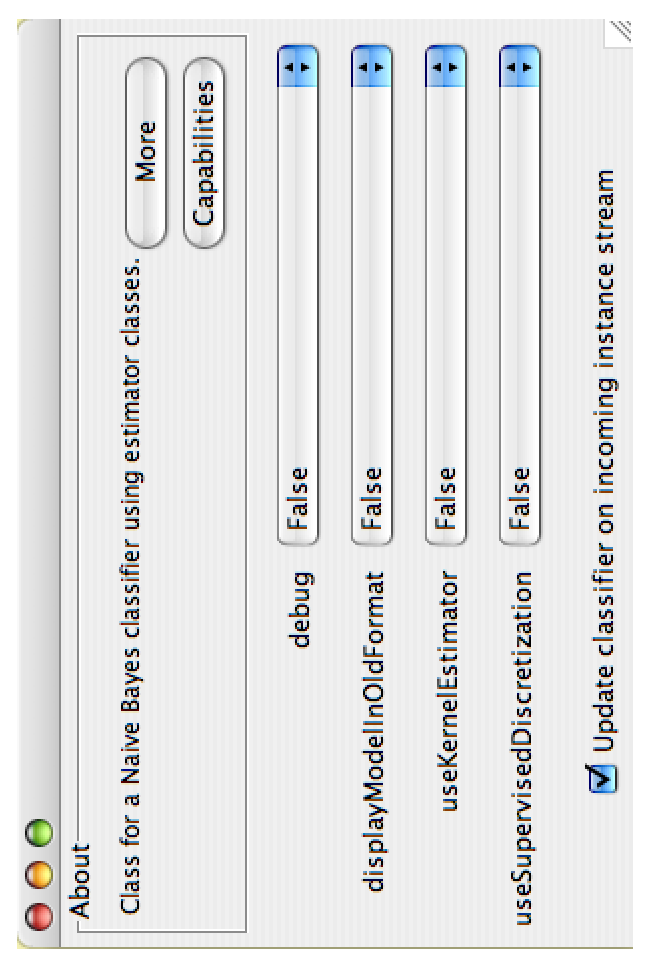
\includegraphics[angle=270,width=12cm]{images/knowledgeflow/IncrementalClassifierConfig.eps}
\end{center}

\newpage
\section{Plugins}

\subsection{Flow components}
The KnowledgeFlow offers the ability to easily add new components via
a plugin mechanism. From Weka 3.7.2 this plugin mechanism has been
subsumed by the package management system and KnowledgeFlow plugins
are no longer installed in \verb=.knowledgeFlow/plugins= in the user's
home directory. Jar files containing plugin components for the
KnowledgeFlow need to be bundled into a package archive. Information
on the structure of a Weka package is given in the Appendix (Chapter
19). In order to tell the KnowledgeFlow which classes in the jar file
to instantiate as components, a second file called
\verb=PlugnManager.props= needs to be included in the top-level
directory of the package. This file contains key/value entries, where
the key specifies an interface or base class, and the value is a
comma-separated list of concrete implementations.  For example, if
we'd developed a new Knowledge Flow step called \verb=FunkyStep=, then
the PluginManager.props file would contain the following entry:

\begin{verbatim}
weka.knowledgeflow.steps.Step=weka.knowledgeflow.steps.FunkyStep
\end{verbatim}

If we had developed a new perspective (see the next section) called
\verb=FunkyPerspective=, then an entry such as the following would
make it appear in the Knowledge Flow (and Workbench).

\begin{verbatim}
weka.gui.Perspective=weka.gui.knowledgeflow.FunkyPerspective
\end{verbatim}


\subsection{Perspectives}
From Weka 3.7.4, the KnowledgeFlow offers a new type of plugin, called
a ``perspective'', that can take over the main UI and add major new
functionality. One example is the \textit{timeSeriesForecasting}
package. This package offer not only a plugin tab for the Explorer,
but also a plugin perspective for the KnowledgeFlow as well. Another
example is the \textit{scatterPlot3D} package which adds a 3D
visualization facility for datasets. Both these perspectives operate
on a set of instances. Instances can be sent to a perspective by
right-clicking over a configured \textit{DataSource} component and
choosing \textit{Send to perspective} from the popup menu.

\begin{center}
  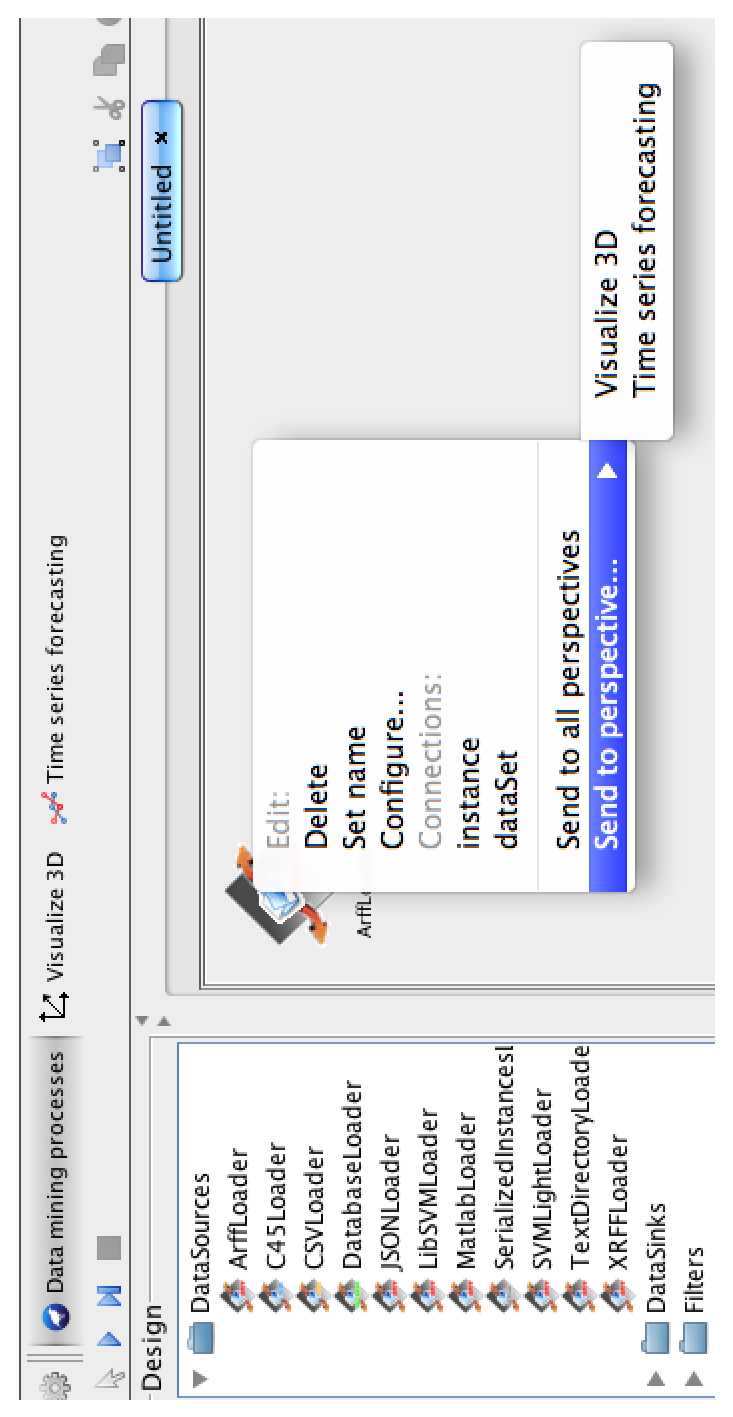
\includegraphics[angle=270,width=12cm]{images/knowledgeflow/sendToPerspective.eps}
\end{center}

\begin{center}
  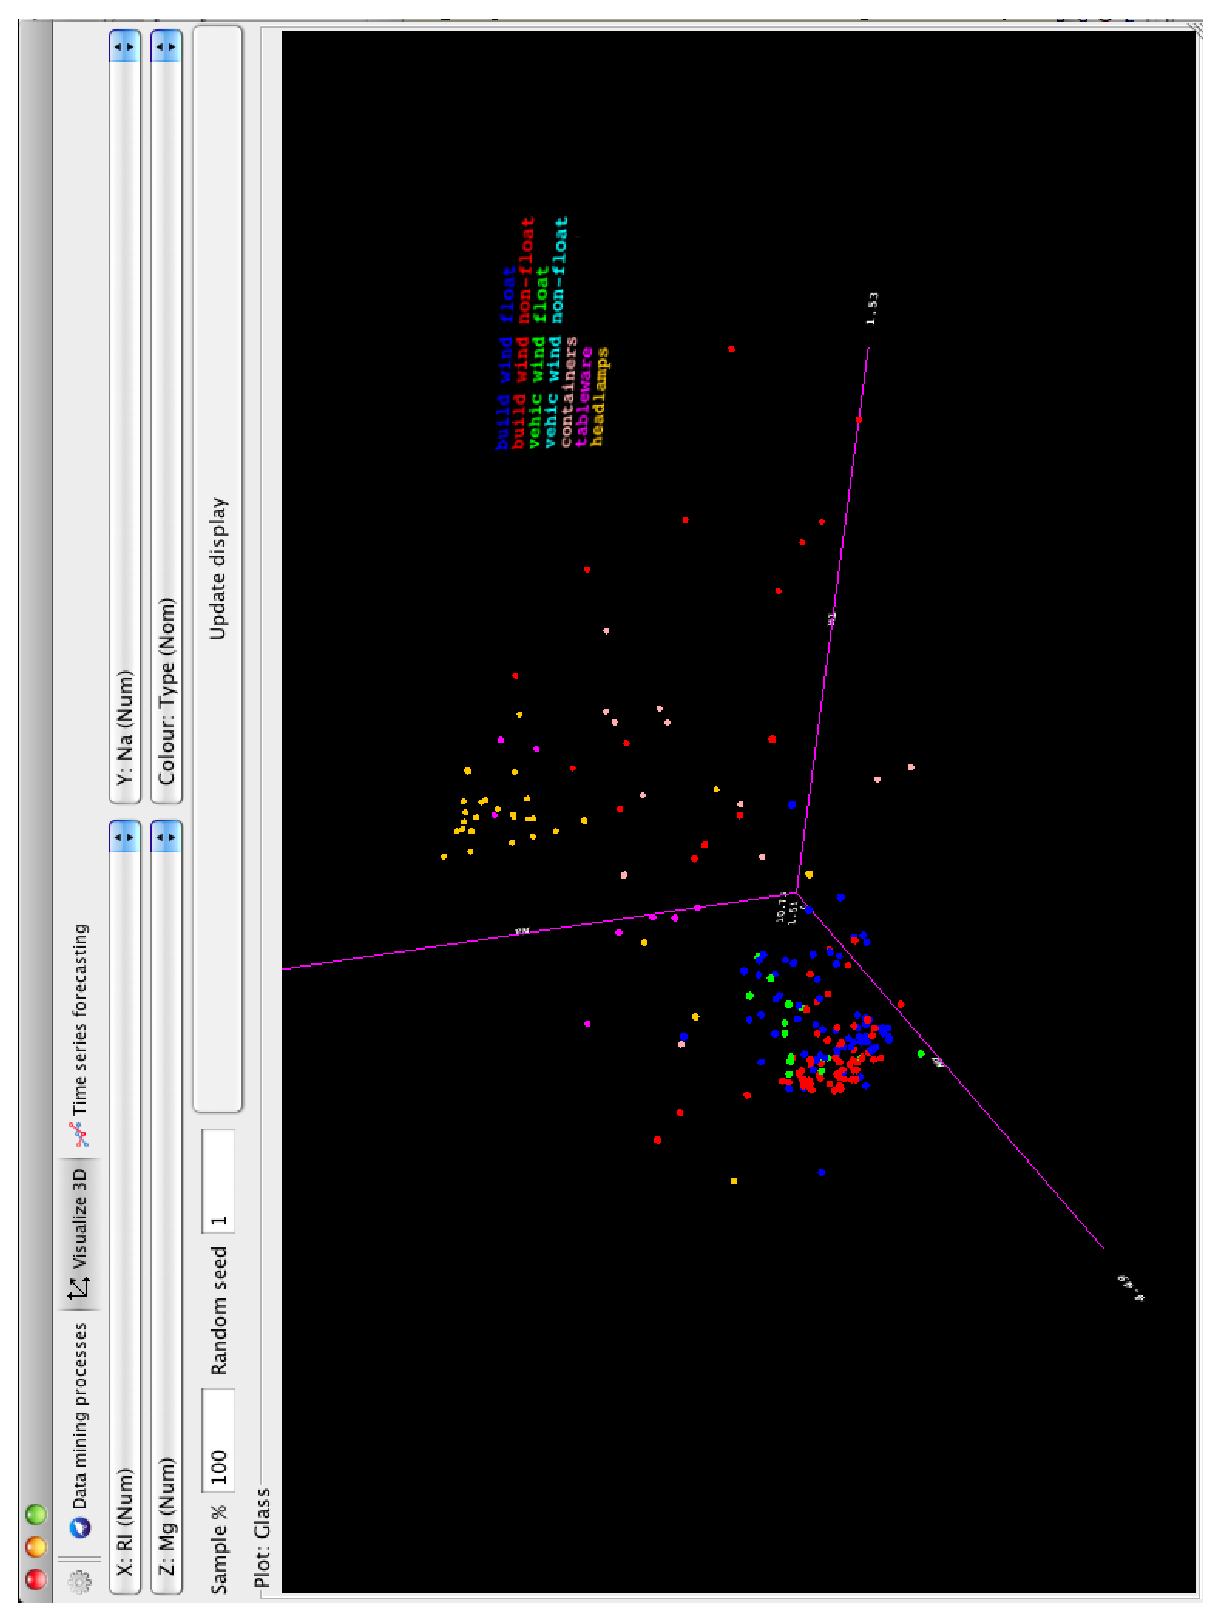
\includegraphics[angle=270,width=12cm]{images/knowledgeflow/scatterPlot3DPerspective.eps}
\end{center}

Several perspectives are built-in to Knowledge Flow and others, such
as the time series environment, can be installed as packages. The
built-in perspectives include: \textit{Attribute summary}, \textit{SQL
  Viewer} and \textit{Scatter plot matrix}. Which perspectives appear
in the toolbar can be configured by clicking the button shaped like a
cog in the upper left-hand corner of the main Knowledge Flow
window. If the Perspectives toolbar is not visible then it can be
shown/hidden by clicking the ``cog with arrow'' button in the main
toolbar at the top right-hand side of the main Knowledge Flow window.


\chapter{ArffViewer}
%
%    This program is free software; you can redistribute it and/or modify
%    it under the terms of the GNU General Public License as published by
%    the Free Software Foundation; either version 2 of the License, or
%    (at your option) any later version.
%
%    This program is distributed in the hope that it will be useful,
%    but WITHOUT ANY WARRANTY; without even the implied warranty of
%    MERCHANTABILITY or FITNESS FOR A PARTICULAR PURPOSE.  See the
%    GNU General Public License for more details.
%
%    You should have received a copy of the GNU General Public License
%    along with this program; if not, write to the Free Software
%    Foundation, Inc., 675 Mass Ave, Cambridge, MA 02139, USA.
%

% Version: $Revision$

The ArffViewer is a little tool for viewing ARFF files in a tabular format. The advantage of this kind of display over the file representation is, that attribute name, type and data are directly associated in columns and not separated in defintion and data part. But the viewer is not only limited to viewing multiple files at once, but also provides simple editing functionality, like sorting and deleting.

\begin{center}
	\epsfig{file=images/arffviewer/arffviewer_main.eps,height=12cm,angle=-90}
\end{center}

\newpage
\section{Menus}
The ArffViewer offers most of its functionality either through the main menu or via popups (table header and table cells). 

Short description of the available menus:
\begin{itemize}
	\item \textbf{File} \\
		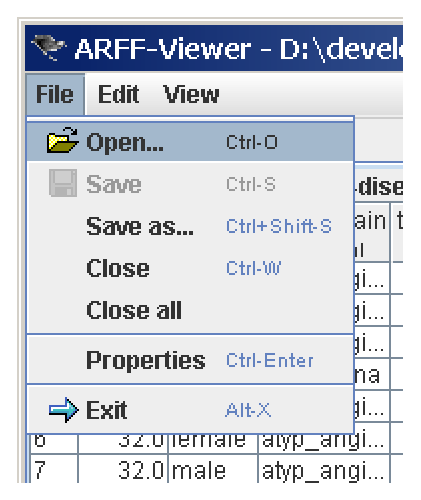
\epsfig{file=images/arffviewer/arffviewer_menu_file.eps,height=4cm} \\
		contains options for opening and closing files, as well as viewing properties about the current file.
	\item \textbf{Edit} \\
		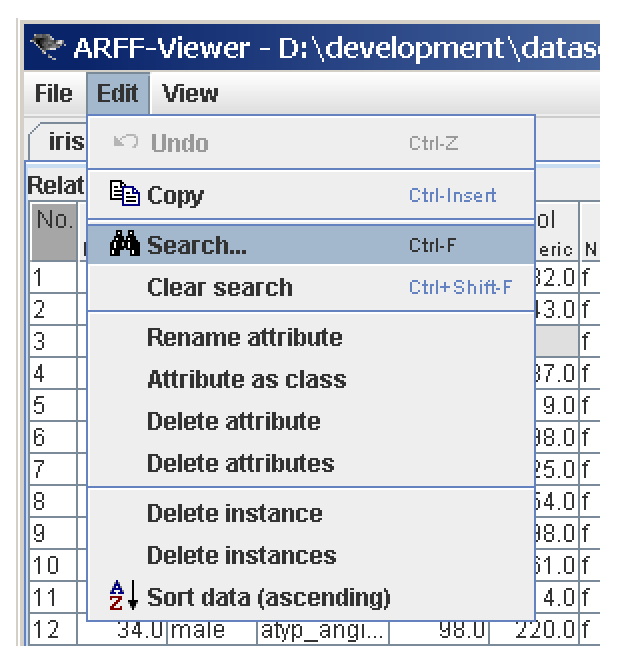
\epsfig{file=images/arffviewer/arffviewer_menu_edit.eps,height=4cm} \\
		allows one to delete attributes/instances, rename attributes, choose a new class attribute, search for certain values in the data and of course undo the modifications.
	\item \textbf{View} \\
		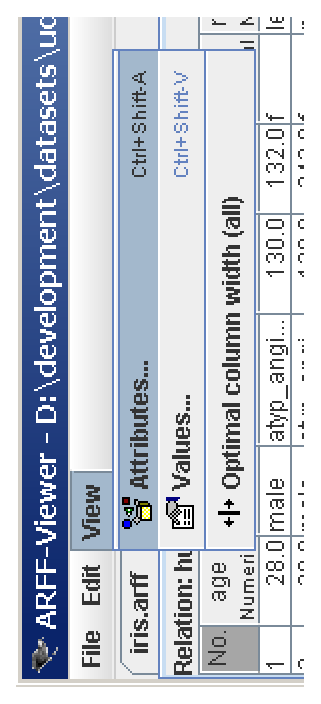
\epsfig{file=images/arffviewer/arffviewer_menu_view.eps,height=4cm,angle=-90} \\
		brings either the chosen attribute into view or displays all the values of an attribute. 
\end{itemize}

After opening a file, by default, the column widths are optimized based on the attribute name and not the content. This is to ensure that overlong cells do not force an enormously wide table, which the user has to reduce with quite some effort. 

\newpage
In the following, screenshots of the table popups:
\begin{center}
	\epsfig{file=images/arffviewer/arffviewer_tableheader_popup.eps,height=12cm,angle=-90}
\end{center}

\begin{center}
	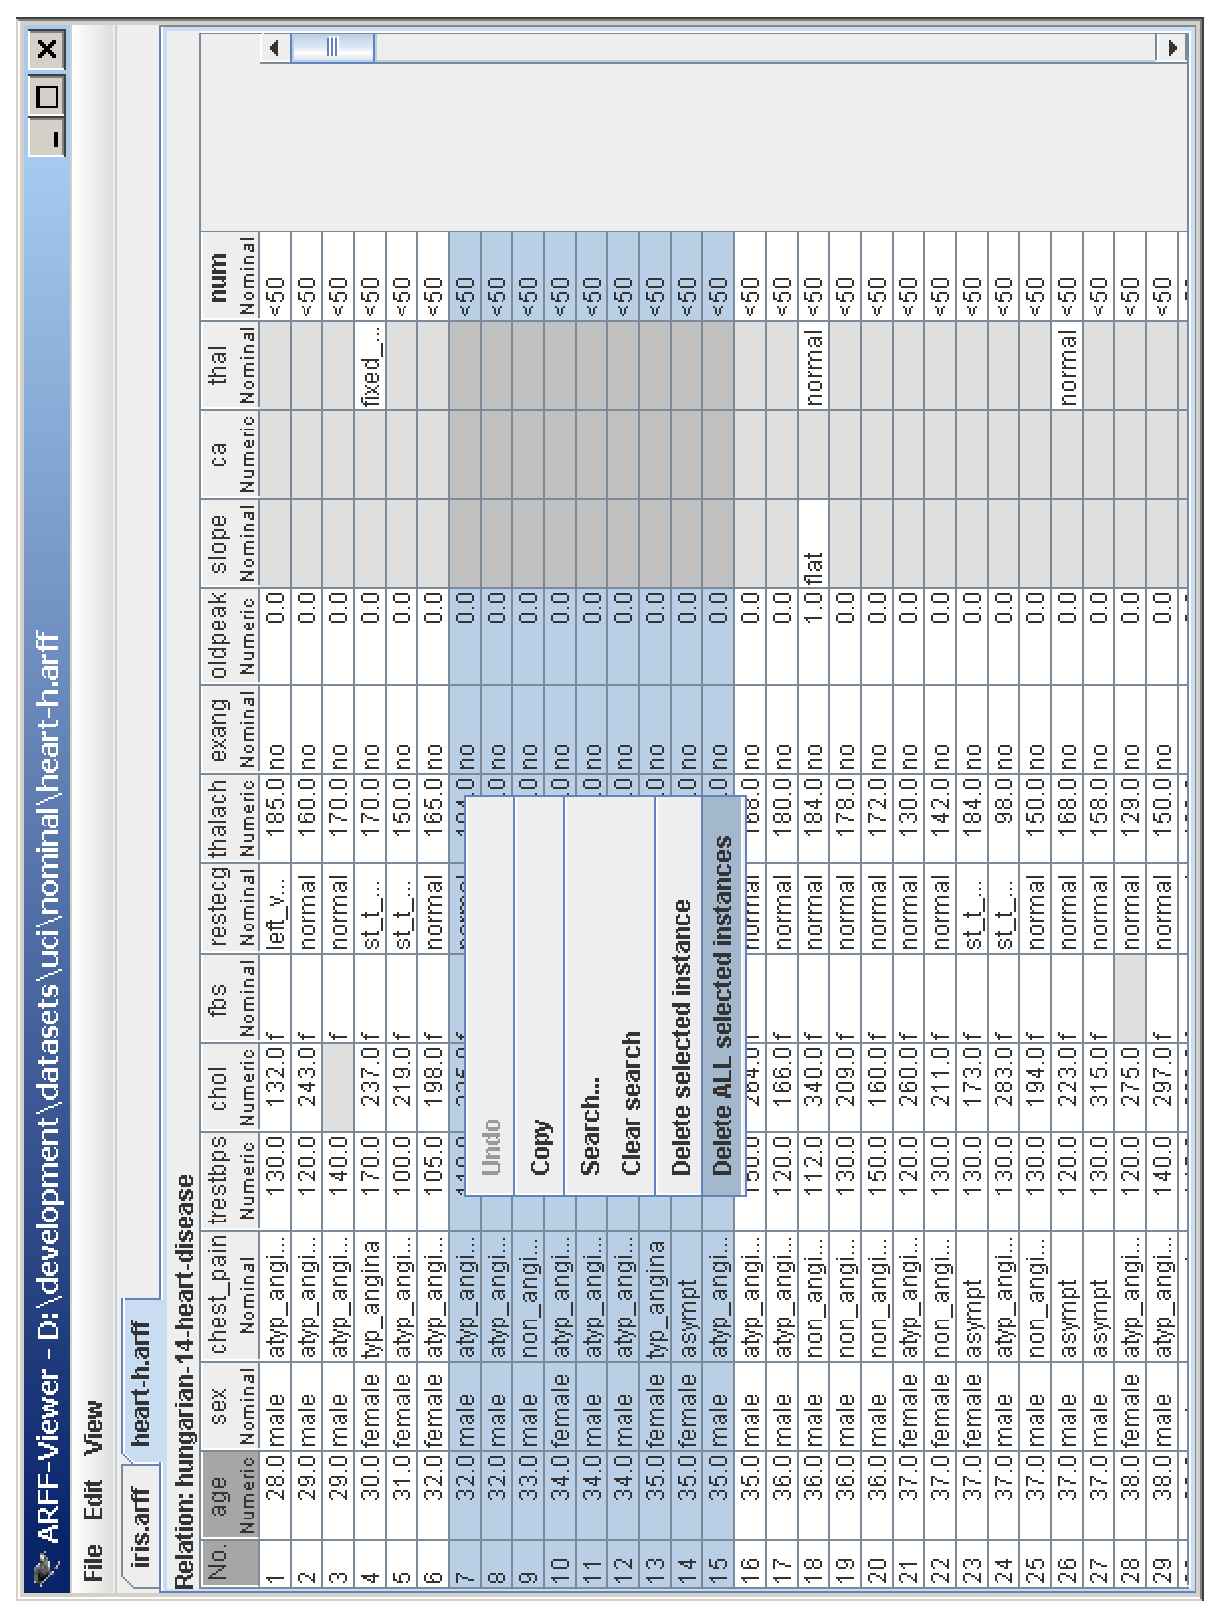
\epsfig{file=images/arffviewer/arffviewer_table_popup.eps,height=12cm,angle=-90}
\end{center}


\newpage
\section{Editing}
Besides the first column, which is the instance index, all cells in the table are editable. Nominal values can be easily modified via dropdown lists, numeric values are edited directly.

\begin{center}
	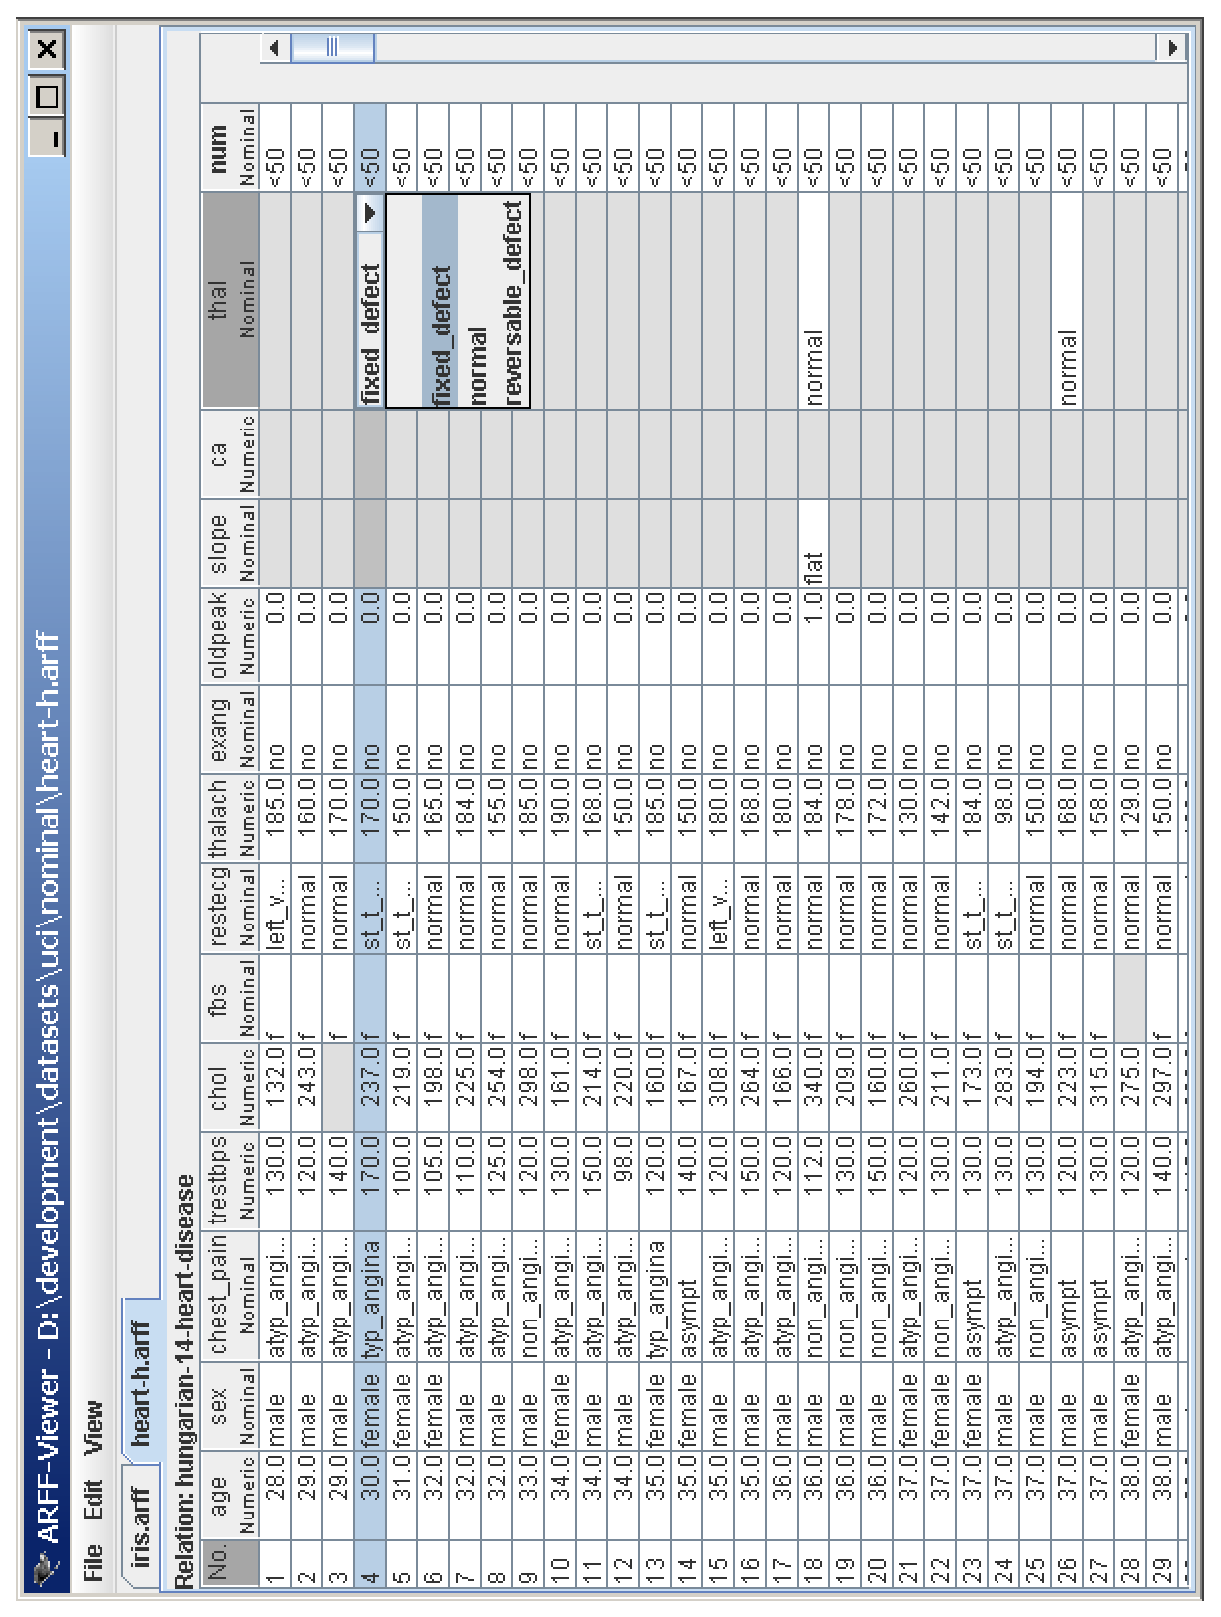
\epsfig{file=images/arffviewer/arffviewer_editing_nominal.eps,height=12cm,angle=-90}
\end{center}

\newpage
For convenience, it is possible to sort the view based on a column (the underlying data is NOT changed; via Edit/Sort data one can sort the data permanently). This enables one to look for specific values, e.g., missing values. To better distinguish missing values from empty cells, the background of cells with missing values is colored grey.

\begin{center}
	\epsfig{file=images/arffviewer/arffviewer_sort_view.eps,height=12cm,angle=-90}
\end{center}


\chapter{Bayesian Network Classifiers}
% Version: $Revision$

\section{Introduction}

Let $U=\{x_1,\ldots,x_n\}$, $n\ge 1$ be a set of variables.
%
A {\em Bayesian network} $B$ over a set of variables $U$ is a {\em
network  structure} $B_S$, which is a directed acyclic graph (DAG)
over $U$ and a set of  probability tables $B_P = \{p(u|pa(u)) | u\in
U\}$ where $pa(u)$ is the set of parents of $u$ in $B_S$. A Bayesian
network represents a probability distributions $P(U) = \prod_{u\in
U}p(u|pa(u))$.

Below, a Bayesian network is shown for the variables in the iris data set.
Note that the links between the nodes class, petallength and petalwidth 
do not form a {\em directed} cycle, so the graph is a proper DAG.

% information about screenshot
% - dataset: iris.arff
% - filter: weka.filters.unsupervised.attribute.Discretize -B 2 -M -1.0 -R first-last
% - classifier: weka.classifiers.bayes.BayesNet -D -Q weka.classifiers.bayes.net.search.local.TabuSearch -- -L 5 -U 10 -P 2 -S BAYES -E weka.classifiers.bayes.net.estimate.SimpleEstimator -- -A 0.5

\begin{center}
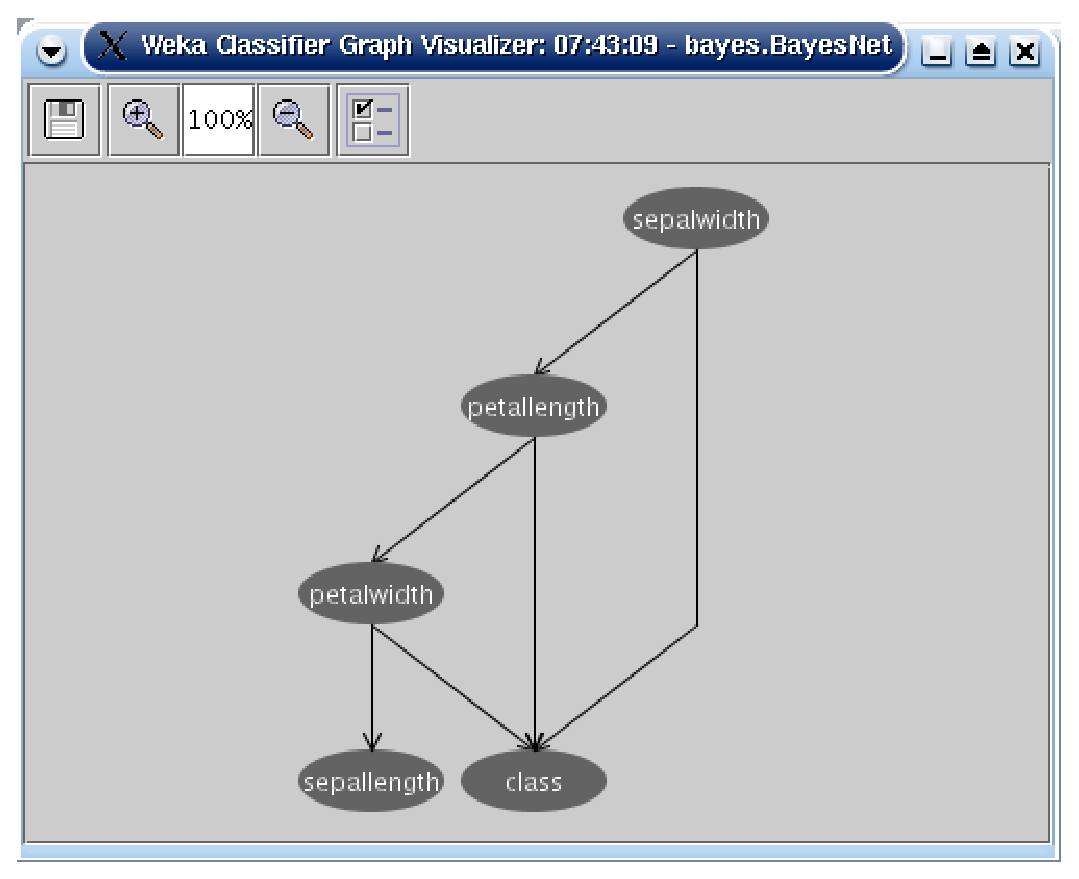
\epsfig{file=images/bayesnet/gui.net.eps,height=7cm}
\end{center}

This picture just shows the network structure of the Bayes net, but for
each of the nodes a probability distribution for the node given its parents
are specified as well. For example, in the Bayes net above there is a conditional distribution
for petallength given the value of class. Since class has no
parents, there is an unconditional distribution for sepalwidth.

\subsection*{Basic assumptions}

The classification task consist of classifying a 
variable $y=x_0$ called the {\em class variable} given a set of variables 
${\bf x} = x_1\ldots x_n$, called {\em attribute variables}. 
%For simplicity, only discrete finite variables with no missing values will be considered.
A classifier $h:{\bf x}\to y$
is a function that maps an instance of $\bf x$ to a value of $y$.
The classifier is learned from a dataset $D$ consisting of samples 
over $({\bf x}, y)$.
%
The learning task consists of finding an appropriate Bayesian network  
given a data set $D$ over $U$.  

All Bayes network algorithms implemented in Weka assume the following
for the data set:
\begin{itemize}
\item all variables are discrete finite variables. If you have a data set
with continuous variables, you can use the following filter to discretize them:\\
{\tt weka.filters.unsupervised.attribute.Discretize} 
\item no instances have missing values. If there are missing values in the
data set, values are filled in using the following filter:\\
{\tt weka.filters.unsupervised.attribute.ReplaceMissingValues}
\end{itemize}

The first step performed by {\tt buildClassifier} is checking if the data set fulfills
those assumptions. If those assumptions are not met, the data set is automatically
filtered and a warning is written to STDERR.\footnote{If there are missing values
in the test data, but not in the training data, the values are filled in in the
test data with a ReplaceMissingValues filter based on the training data.}

\subsection*{Inference algorithm}

To use a Bayesian network as a classifier, one simply calculates $argmax_yP(y|{\bf x})$
using the distribution $P(U)$ represented by the Bayesian network. 
Now note that

\begin{eqnarray}
P(y|{\bf x})&=&P(U)/P({\bf x})\nonumber\\
&\propto& P(U)\nonumber\\
&=&\prod_{u\in U}p(u|pa(u))\label{eq.infer}%\\
\end{eqnarray}

And since all variables in ${\bf x}$ are known, we do not need complicated inference
algorithms, but just calculate (\ref{eq.infer}) for all class values.

\subsection*{Learning algorithms}

The dual nature of a Bayesian network makes learning a Bayesian
network as a two stage process a natural division: first learn a
network structure, then learn the probability tables.

There are various approaches to structure learning and in Weka, the
following areas are distinguished:

\begin{itemize}
\item {\em local score metrics}: 
Learning a network structure $B_S$ can be considered an optimization
problem where a quality measure of a network structure given the
training data $Q(B_S|D)$ needs to be maximized. The quality measure
can be based on a Bayesian approach,  minimum description length,
information and other criteria. Those metrics have the practical property
that the score of the whole network can be decomposed as the sum 
(or product) of the score of the individual nodes. This allows for 
local scoring and thus local search methods.

\item {\em conditional independence tests}:
These methods mainly stem from the goal of uncovering causal structure.
The assumption is that there is a network structure that exactly represents
the independencies in the distribution that generated the data. Then it
follows that if a (conditional) independency can be identified in the data
between two variables that there is no arrow between those two 
variables. Once locations of edges are identified, the direction of the edges
is assigned such that conditional independencies in the data are properly
represented.

\item {\em global score metrics}:
A natural way to measure how well a Bayesian network performs on a
given data set is to predict its future performance by estimating
expected utilities, such as classification accuracy.  Cross-validation
provides an out of sample evaluation method to facilitate this by
repeatedly splitting the data in training and validation sets.  A
Bayesian network structure  can be evaluated by estimating the
network's parameters from the training set and the resulting Bayesian
network's performance determined against the validation set.  The
average performance of the Bayesian network over the validation sets
provides a metric for the quality of the network.

Cross-validation differs from local scoring metrics  in that the quality
of a network structure often cannot be decomposed in the scores of the
individual nodes. So, the whole network needs to be considered in order
to determine the score.

\item {\em fixed structure}:
Finally, there are a few methods so that a structure can be fixed, for
example, by reading it from an XML BIF file\footnote{See
{\sf \url{http://www-2.cs.cmu.edu/\~fgcozman/Research/InterchangeFormat/}{}}
for details on XML BIF.}.
\end{itemize}

For each of these areas, different search algorithms are implemented in 
Weka, such as hill climbing, simulated annealing and tabu search.

Once a good network structure is identified, the conditional probability
tables for each of the variables can be estimated.

You can select a Bayes net classifier by clicking the classifier 'Choose' button in 
the Weka explorer, experimenter or knowledge flow and find {\tt BayesNet}
under the {\tt weka.classifiers.bayes} package (see below).

\begin{center}
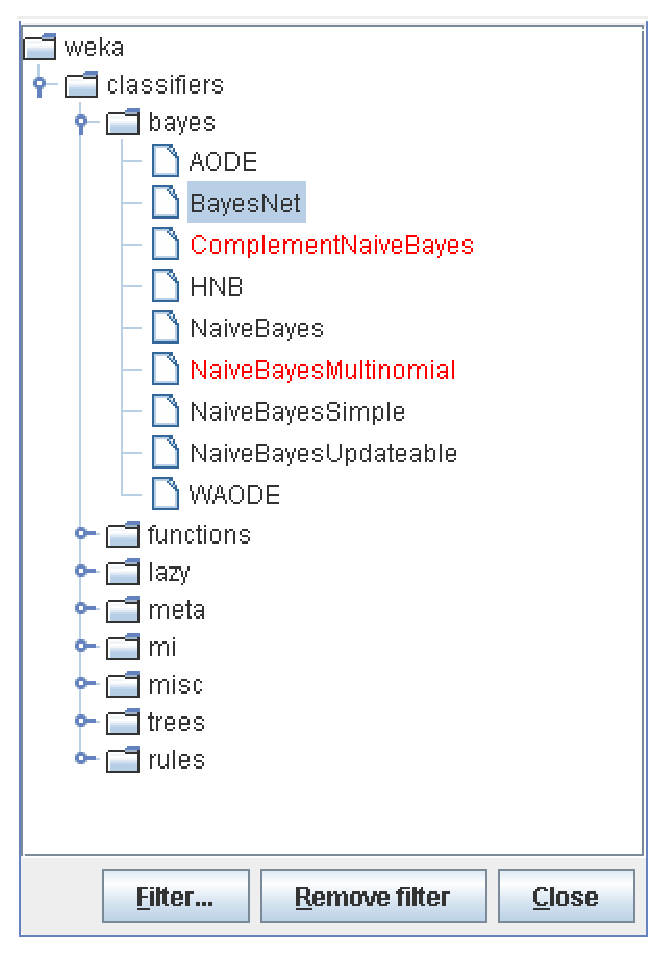
\epsfig{file=images/bayesnet/select.eps,height=7cm}
\end{center}

The Bayes net classifier has the following options:

\begin{center}
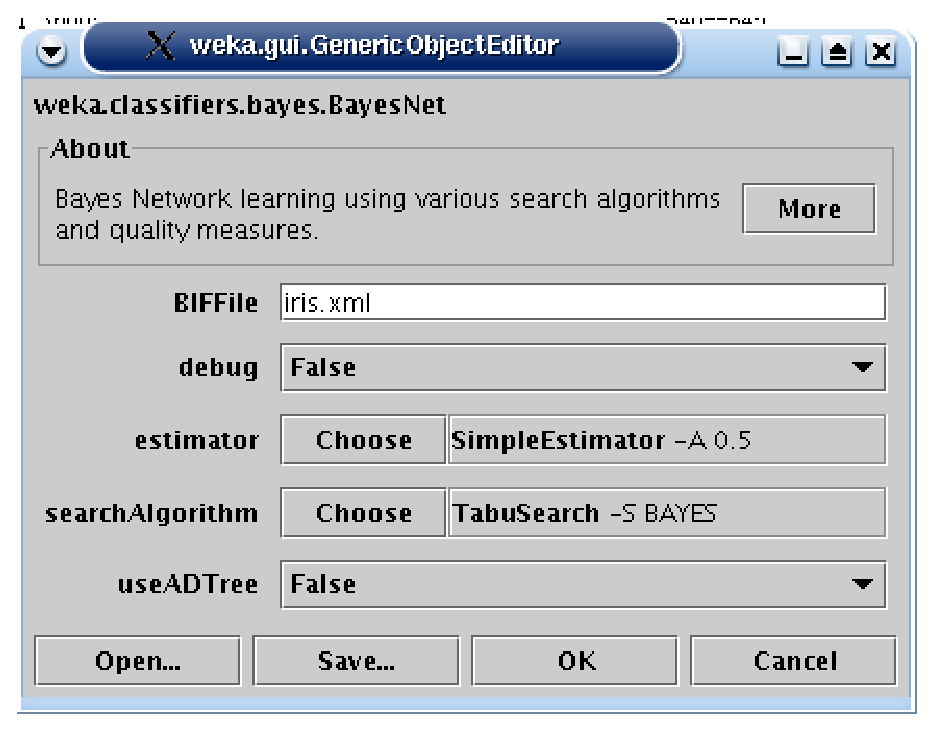
\epsfig{file=images/bayesnet/bayesnet.options.eps,height=7cm}
\end{center}

The {\tt BIFFile} option can be used to specify a Bayes network stored in
file in BIF format. When the {\tt toString()} method is called after learning the
Bayes network, extra statistics (like extra and missing arcs) are printed 
comparing the network learned with the one on file.

The {\tt searchAlgorithm} option can be used to select a structure learning
algorithm and specify its options.

The {\tt estimator} option can be used to select the method for estimating the
conditional probability distributions (Section \ref{sec.estimate}).

When setting the {\tt useADTree} option to \textbf{true}, counts are calculated using the
ADTree algorithm of Moore \cite{Moore}. Since I have not noticed a lot of 
improvement for small data sets, it is set off by default.
Note that this ADTree algorithm is different from the ADTree classifier algorithm
from {\tt weka.classifiers.tree.ADTree}.

The {\tt debug} option has no effect.

\section{Local score based structure learning\label{sec.score}}

Distinguish score metrics (Section 2.1) and search algorithms (Section 2.2).
A local score based structure learning can be selected by choosing one in the
{\tt weka.classifiers.bayes.net.search.local} package.

\begin{center}
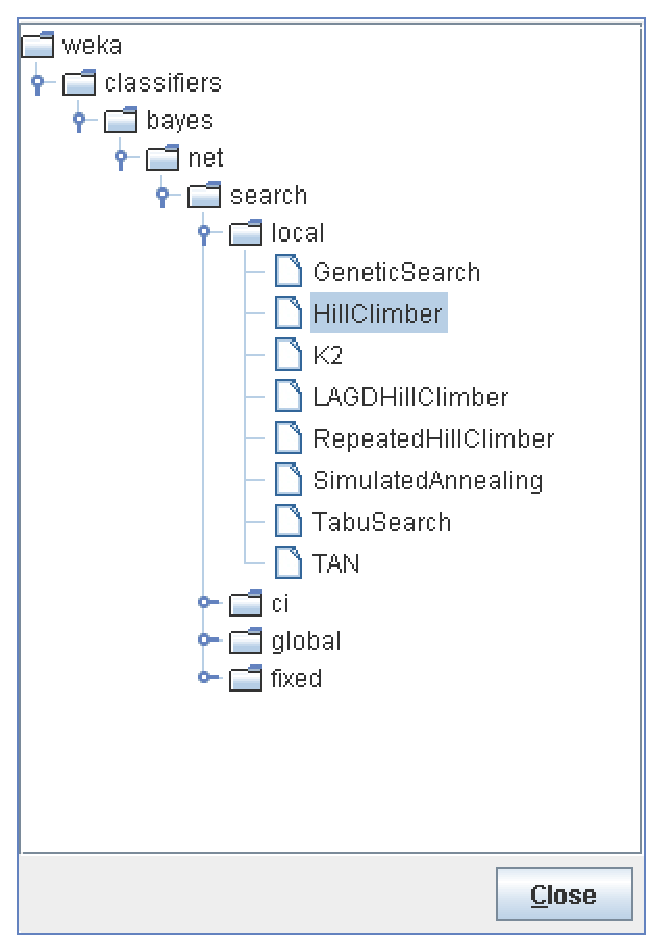
\epsfig{file=images/bayesnet/local.algorithms.eps,height=8cm}
\end{center}


Local score based algorithms have the following options in common:\\
{\tt initAsNaiveBayes} if set {\bf true} (default), the initial network structure used
for starting the traversal of the search space is a naive Bayes network 
structure. That is, a structure with arrows from the class variable to
each of the attribute variables.\\
If set {\bf false}, an empty network structure will be used (i.e., no arrows at all).\\
{\tt markovBlanketClassifier} (\textbf{false} by default) if set {\bf true},
at the end of the traversal of the search space, a heuristic is used
to ensure each of the attributes are in the Markov blanket of the 
classifier node. If a node is already in the Markov blanket (i.e., is
a parent, child of sibling of the classifier node) nothing happens,
otherwise an arrow is added.\\
If set to {\bf false} no such arrows are added.\\
{\tt scoreType} determines the score metric used (see Section 2.1
for details). Currently, K2, BDe, AIC, Entropy and MDL are implemented.\\
{\tt maxNrOfParents} is an upper bound on the number of parents of each of the
nodes in the network structure learned.

\subsection{Local score metrics \label{sec.score.metric}}

We use the following conventions to identify counts in the database
$D$ and a network structure $B_S$.  Let $r_i$ ($1\le i\le n$) be the
cardinality of $x_i$.  We use $q_i$ to denote the cardinality of the
parent set of $x_i$ in $B_S$,  that is, the number of different values
to which the parents of $x_i$ can be  instantiated.  So, $q_i$ can be
calculated as the product of cardinalities of nodes in $pa(x_i)$,
$q_i=\prod_{x_j\in pa(x_i)}r_j$.  Note $pa(x_i)=\emptyset$ implies
$q_i=1$.
%
 We use $N_{ij}$ ($1\le i\le n$, $1\le j\le q_i$) to denote the number
of records in $D$ for which $pa(x_i)$ takes its $j$th value.%
We use $N_{ijk}$ ($1\le i\le n$, $1\le j\le q_i$, $1\le k\le r_i$) to
denote the number of records in $D$ for which $pa(x_i)$ takes its
$j$th value and for which $x_i$ takes its $k$th value.
%
So, $N_{ij}=\sum_{k=1}^{r_i}N_{ijk}$.  We use $N$ to denote the number
of records in $D$.

Let the {\em entropy metric} $H(B_S,D)$ of a network structure and database
be defined as
\begin{equation}\label{eq.H}
 H(B_S,D)=-N\sum_{i=1}^n\sum_{j=1}^{q_i}\sum_{k=1}^{r_i}\frac{N_{ijk}}{N}\log\frac{N_{ijk}}{N_{ij}}
\end{equation}
and the {\em number of parameters} $K$ as
\begin{equation}\label{eq.K}
K=\sum_{i=1}^n(r_i-1)\cdot q_i
\end{equation}

{\bf AIC metric} The AIC metric $Q_{AIC}(B_S,D)$ of a Bayesian network
structure $B_S$ for a database $D$ is
\begin{equation}\label{eq.AIC}
Q_{AIC}(B_S,D) = H(B_S,D)+K
\end{equation}
A term $P(B_S)$ can be added \cite{bouck1995} representing prior
information  over network structures, but will be ignored for
simplicity in the Weka implementation.

%{\bf RIC metric} The Risk Inflation Criterion (RIC) metric $Q_{RIC}(B_S,D)$ is
%\begin{equation}\label{eq.AIC}
%Q_{RIC}(B_S,D) = H(B_S,D)+log(K)
%\end{equation}
% NOTE: CANNOT DECOMPOSE INTO LOCAL SCORING METRIC

{\bf MDL metric} 
The minimum description length metric $Q_{MDL}(B_S,D)$
of a Bayesian network structure $B_S$ for a database $D$ is
is defined as

\begin{equation}\label{eq.MDL}
Q_{MDL}(B_S,D) = H(B_S,D)+\frac{K}{2}\log N
\end{equation}

{\bf Bayesian metric}
The Bayesian metric of a Bayesian network structure $B_D$ for a database $D$ is
$$
Q_{Bayes}(B_S,D) = P(B_S)\prod_{i=0}^n\prod_{j=1}^{q_i}\frac{\Gamma(N_{ij}')}{\Gamma(N_{ij}'+N_{ij})}
\prod_{k=1}^{r_i}\frac{\Gamma(N_{ijk}'+N_{ijk})}{\Gamma(N_{ijk}')}
$$
where $P(B_S)$ is the prior on the network structure (taken to be constant hence ignored 
in the Weka implementation) and $\Gamma(.)$ the gamma-function. $N_{ij}'$ and $N_{ijk}'$
represent choices of priors on counts restricted by 
$N_{ij}'=\sum_{k=1}^{r_i}N_{ijk}'$. With $N_{ijk}'=1$ (and thus $N_{ij}'=r_i$), 
we obtain the K2 metric \cite{CooperHerskovits1992}
$$
Q_{K2}(B_S,D) = P(B_S)\prod_{i=0}^n\prod_{j=1}^{q_i}\frac{(r_i-1)!}{(r_i-1+N_{ij})!}
\prod_{k=1}^{r_i}N_{ijk}!
$$
With $N_{ijk}'=1/r_i\cdot q_i$ (and thus $N_{ij}'=1/q_i$), we obtain the {\bf BDe metric}
\cite{heckerman95}.


\subsection{Search algorithms \label{sec.score.search}}

The following search algorithms are implemented for local score metrics;
\begin{itemize}
\item \textit{K2} \cite{CooperHerskovits1992}: 
hill climbing add arcs with a fixed ordering of variables.\\
Specific option: {\tt randomOrder} if {\bf true} a random ordering of
the nodes is made at the beginning of the search. If {\bf false} (default)
the ordering in the data set is used. The only exception in both cases is that
in case the initial network is a naive Bayes network ({\tt initAsNaiveBayes}
set \textbf{true}) the class variable is made first in the ordering.
\item \textit{Hill Climbing} 
\cite{Buntine1996}: 
hill climbing adding and deleting arcs with no fixed ordering of variables.\\
{\tt useArcReversal} if \textbf{true}, also arc reversals are consider when determining
the next step to make.
\item \textit{Repeated Hill Climber} starts with a randomly generated network and
then applies hill climber to reach a local optimum. The best network found is
returned.\\
{\tt useArcReversal} option as for Hill Climber.
\item \textit{LAGD Hill Climbing} does hill climbing with look ahead on a limited set of 
best scoring steps, implemented by Manuel Neubach. The number of look ahead steps and number of steps considered
for look ahead are configurable.
\item \textit{TAN} \cite{ChengGreiner1999,friedman97}:
\textit{T}ree \textit{A}ugmented \textit{N}aive Bayes where the tree is formed by calculating the
maximum weight spanning tree using Chow and Liu algorithm \cite{chow1968}.\\
No specific options.
\item \textit{Simulated annealing} \cite{bouck1995}:
using adding and deleting arrows.\\
The algorithm randomly generates a candidate network $B_S'$ close to the current
network $B_S$. It accepts the network if it is better than the current, i.e.,
$Q(B_S',D) > Q(B_S,D)$. 
Otherwise, it accepts the candidate with probability 
$$e^{t_i \cdot(Q(B_S',D) -Q(B_S,D))}$$
where $t_i$ is the temperature at iteration $i$.
The temperature starts at $t_0$ and is slowly decreases with each iteration. 

\begin{center}
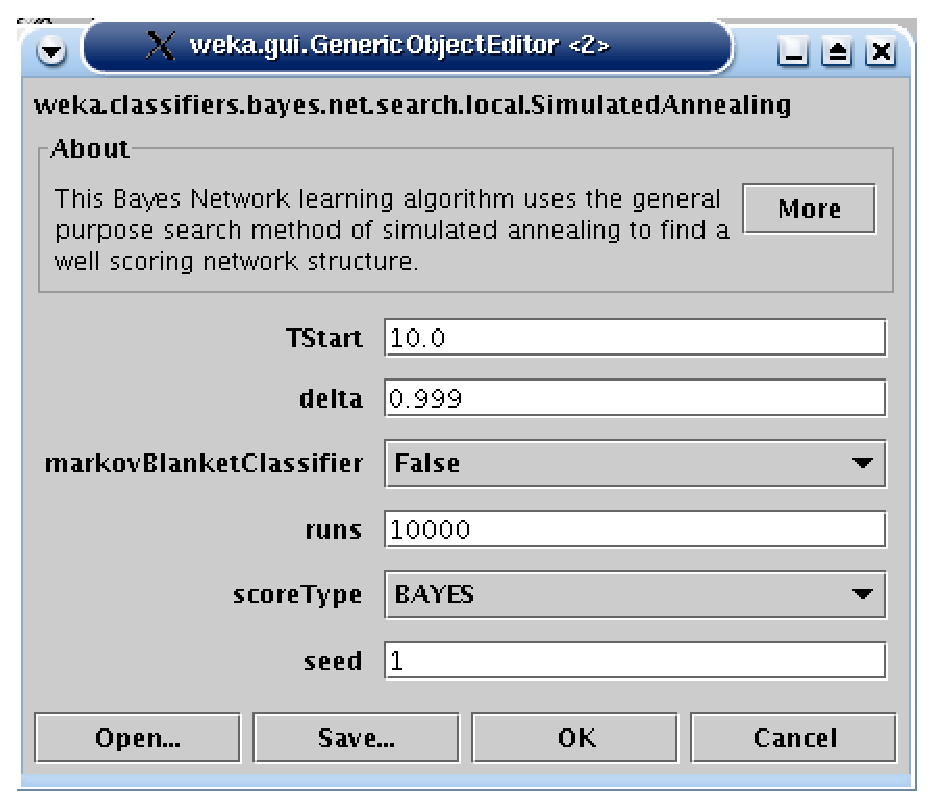
\epsfig{file=images/bayesnet/score.sa.eps,height=5cm}
\end{center}

Specific options:\\
{\tt TStart} start temperature $t_0$.\\
{\tt delta} is the factor $\delta$ used to update the temperature, so $t_{i+1}=t_i \cdot \delta$.\\
{\tt runs} number of iterations used to traverse the search space.\\
{\tt seed} is the initialization value for the random number generator.\\

\item \textit{Tabu search} \cite{bouck1995}:
using adding and deleting arrows.\\
Tabu search performs hill climbing until it hits a local optimum.
Then it steps to the least worse candidate in the neighborhood. However,
it does not consider points in the neighborhood it just visited in the
last $tl$ steps. These steps are stored in a so called tabu-list.

\begin{center}
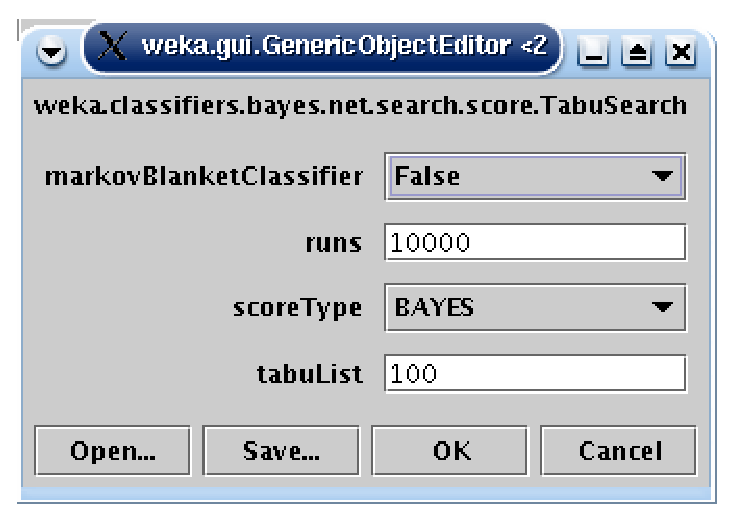
\epsfig{file=images/bayesnet/score.tabu.eps,height=5cm}
\end{center}

Specific options: \\
{\tt runs} is the number of iterations used to traverse the search space.\\
{\tt tabuList} is the length $tl$ of the tabu list.

\item \textit{Genetic search}: applies a simple implementation of a genetic search algorithm
to network structure learning. A Bayes net structure is represented by a array
of $n\cdot n$ ($n$ = number of nodes) bits where bit $i\cdot n + j$ represents whether
there is an arrow from node $j\to i$.\\

\begin{center}
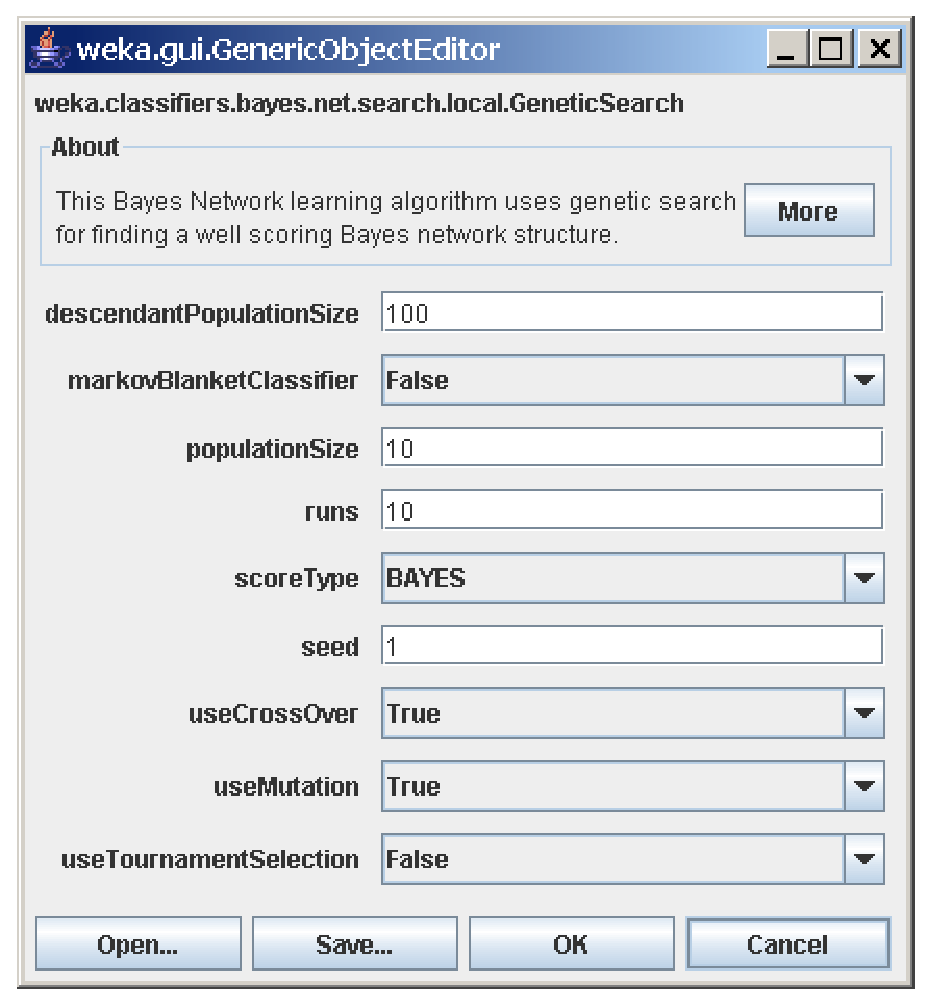
\epsfig{file=images/bayesnet/score.genetic.eps,height=8cm}
\end{center}

Specific options:\\
{\tt populationSize} is the size of the population selected in each generation.\\
{\tt descendantPopulationSize} is the number of offspring generated in each generation.\\
{\tt runs} is the number of generation to generate.\\
{\tt seed} is the initialization value for the random number generator.\\
{\tt useMutation} flag to indicate whether mutation should be used. Mutation is applied by
randomly adding or deleting a single arc.\\
{\tt useCrossOver} flag to indicate whether cross-over should be used. Cross-over is applied
by randomly picking an index $k$ in the bit representation and selecting the first $k$ bits
from one and the remainder from another network structure in the population.
At least one of \texttt{useMutation} and \texttt{useCrossOver} should be set to \textbf{true}.\\
{\tt useTournamentSelection} when \textbf{false}, the best performing networks are selected from
the descendant population to form the population of the next generation. 
When \textbf{true}, tournament selection is used. Tournament selection randomly chooses two
individuals from the descendant population and selects the one that performs best.\\
\end{itemize}

\section{Conditional independence test based structure learning}

Conditional independence tests in Weka are slightly different from the
standard tests described in the literature. To test whether variables
$x$ and $y$ are conditionally independent given a set of variables $Z$,
a network structure with arrows $\forall_{z\in Z}z \to y$ is compared with
one with arrows $\{x\to y\} \cup \forall_{z\in Z}z \to y$. 
A test is performed by using any of the score metrics described in Section 
2.1.

\begin{center}
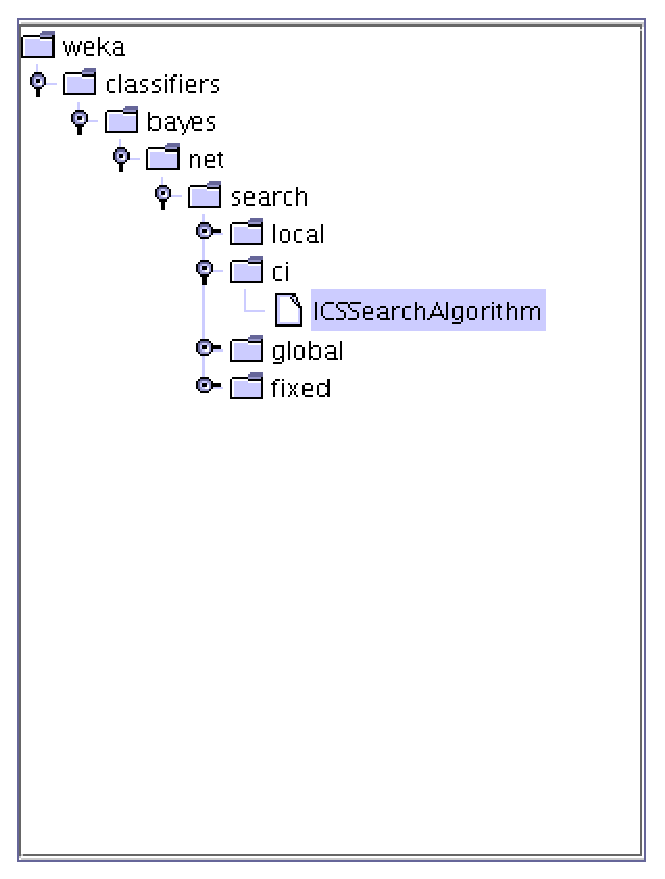
\epsfig{file=images/bayesnet/ci.algorithms.eps,height=8cm}
\end{center}

At the moment, only the ICS  \cite{verma}and CI algorithm are implemented. 

The ICS algorithm makes two steps, first find a skeleton (the undirected graph with edges $iff$ there
is an arrow in network structure) and second direct all the edges in the skeleton
to get a DAG.

Starting with a complete undirected graph, we try to find conditional independencies
$\langle x,y|Z\rangle$ in the data. For each pair of nodes $x$, $y$, we consider sets
$Z$ starting with cardinality $0$, then $1$ up to a user defined maximum. Furthermore,
the set $Z$ is a subset of nodes that are neighbors of both $x$ and $y$. If an
independency is identified, the edge between $x$ and $y$ is removed from the skeleton.

The first step in directing arrows is to check for every configuration $x--z--y$
where $x$ and $y$ not connected in the skeleton whether $z$ is in the set $Z$ of
variables that justified removing the link between $x$ and $y$ (cached in the
first step). If $z$ is not in $Z$, we can assign direction $x\to z\leftarrow y$.

Finally, a set of graphical rules is applied \cite{verma} to direct the remaining
arrows.
\begin{verbatim}
           Rule 1: i->j--k & i-/-k => j->k
           Rule 2: i->j->k & i--k => i->k
           Rule 3  m
                         /|\
                        i | k  => m->j
                i->j<-k  \|/
                          j
        
           Rule 4  m
                         / \
                        i---k  => i->m & k->m
                  i->j   \ /
                          j
           Rule 5: if no edges are directed then take a random one (first we can find)
\end{verbatim}

The ICS algorithm comes with the following options.

\begin{center}
\epsfig{file=images/bayesnet/ci.ics.eps,height=5cm}
\end{center}

Since the ICS algorithm is focused on recovering causal structure, instead of 
finding the optimal classifier, the Markov blanket correction can be made 
afterwards.\\
\\
Specific options:\\
The {\tt maxCardinality} option determines the largest subset of $Z$ to be 
considered in conditional independence tests $\langle x,y|Z\rangle$. \\
The {\tt scoreType} option is used to select the scoring metric.

\section{Global score metric based structure learning}

\begin{center}
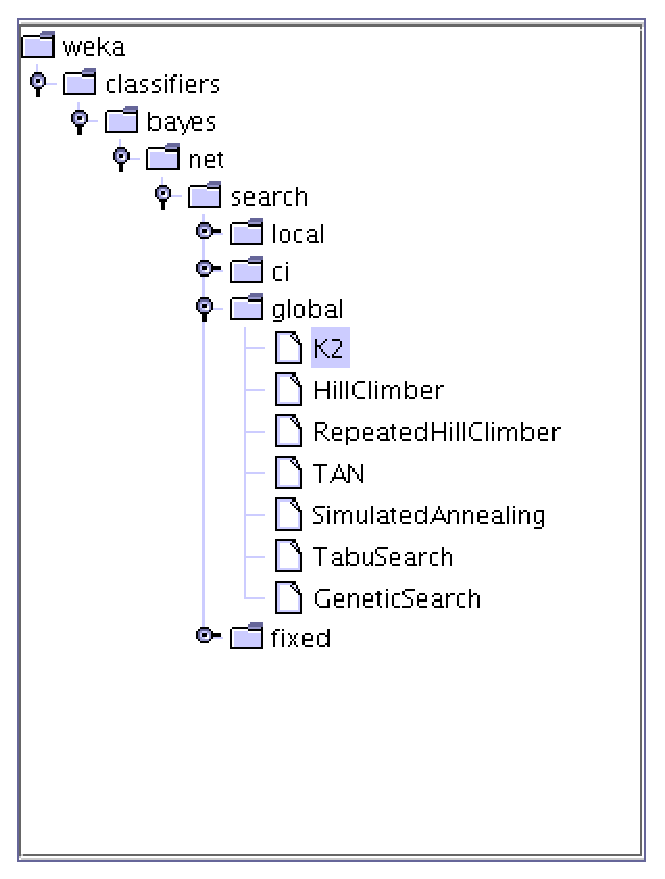
\epsfig{file=images/bayesnet/global.algorithms.eps,height=8cm}
\end{center}

Common options for cross-validation based algorithms are: \\
{\tt initAsNaiveBayes}, {\tt markovBlanketClassifier} and {\tt maxNrOfParents}
(see Section \ref{sec.score} for description).

Further, for each of the cross-validation based algorithms the {\tt CVType} can be
chosen out of the following:

\begin{itemize}
\item {\em Leave one out cross-validation (loo-cv)} selects $m=N$ training sets 
simply by taking the data set $D$ and removing the $i$th record for training 
set $D_i^t$. The validation set consist of just the $i$th single record. 
Loo-cv does not always produce accurate performance estimates. 

\item {\em K-fold cross-validation (k-fold cv)} splits the data $D$ in $m$ approximately 
equal parts $D_1,\ldots,D_m$. Training set $D_i^t$ is obtained by removing part 
$D_i$ from $D$. Typical values for $m$ are 5, 10 and 20. With $m=N$, k-fold cross-validation becomes loo-cv. 

\item {\em Cumulative cross-validation (cumulative cv)} starts with an empty data
set and adds instances item by item from $D$. After each time an item is added
the next item to be added is classified using the then current state of the
Bayes network.
\end{itemize}

Finally, the {\tt useProb} flag indicates whether the accuracy of the classifier
should be estimated using the zero-one loss (if set to {\bf false}) or using
the estimated probability of the class.

\begin{center}
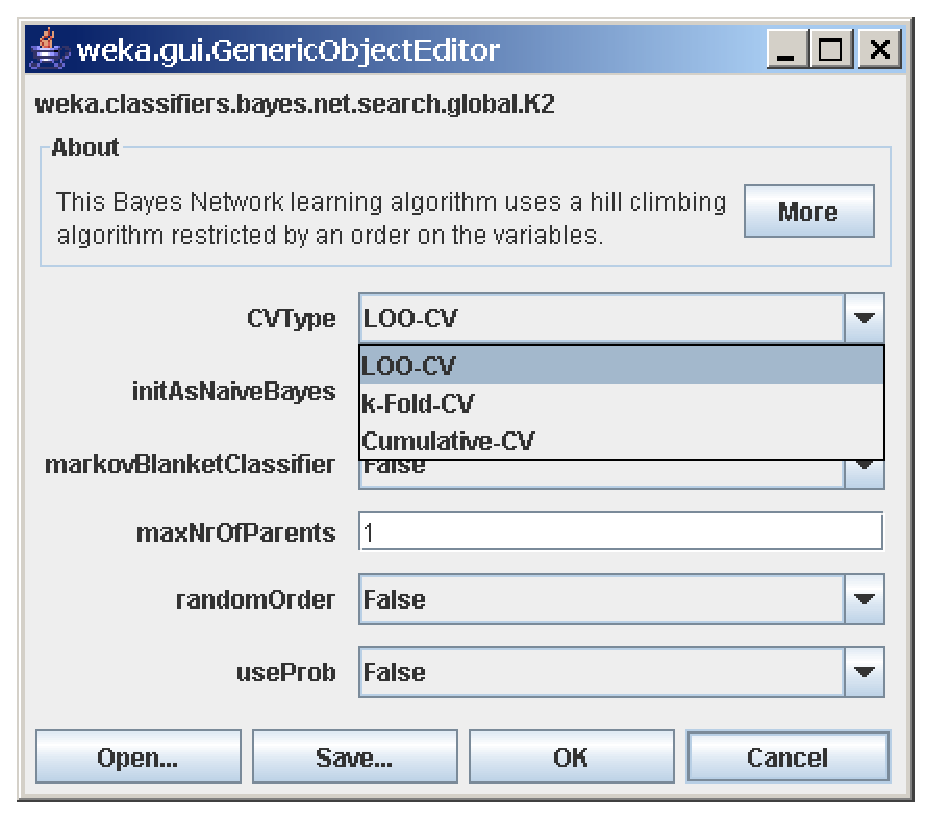
\epsfig{file=images/bayesnet/global.k2.eps,height=6cm}
\end{center}

The following search algorithms are implemented: K2, HillClimbing, RepeatedHillClimber,
TAN, Tabu Search, Simulated Annealing and Genetic Search. See Section \ref{sec.score} for
a description of the specific options for those algorithms.

\section{Fixed structure 'learning'}

The structure learning step can be skipped by selecting a fixed network
structure. There are two methods of getting a fixed structure: just make
it a naive Bayes network, or reading it from a file in XML BIF format.

\begin{center}
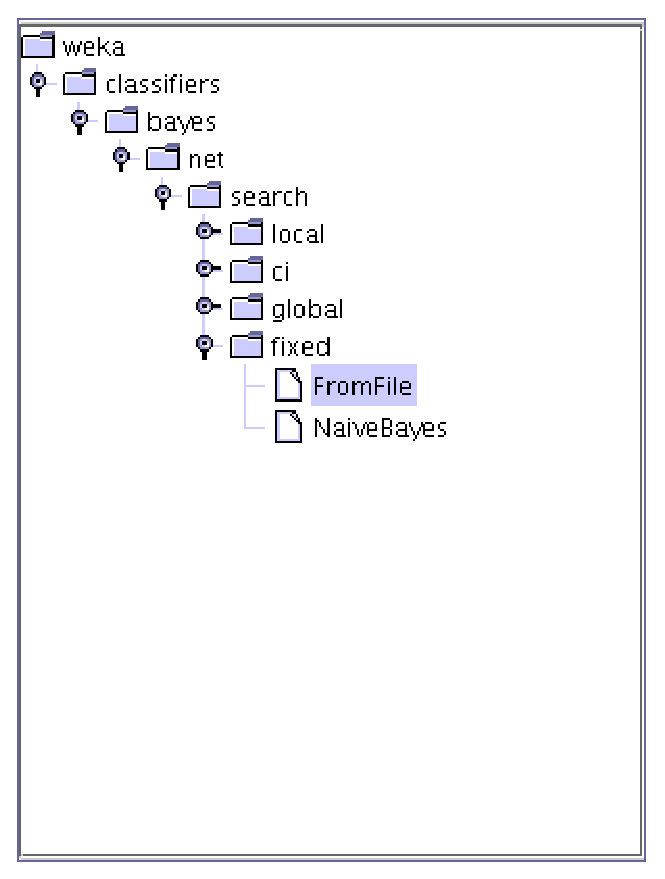
\epsfig{file=images/bayesnet/fixed.algorithms.eps,height=8cm}
\end{center}

\section{Distribution learning\label{sec.estimate}}

Once the network structure is learned, you can choose how to learn the probability
tables selecting a class in the {\tt weka.classifiers.bayes.net.estimate} package.

\begin{center}
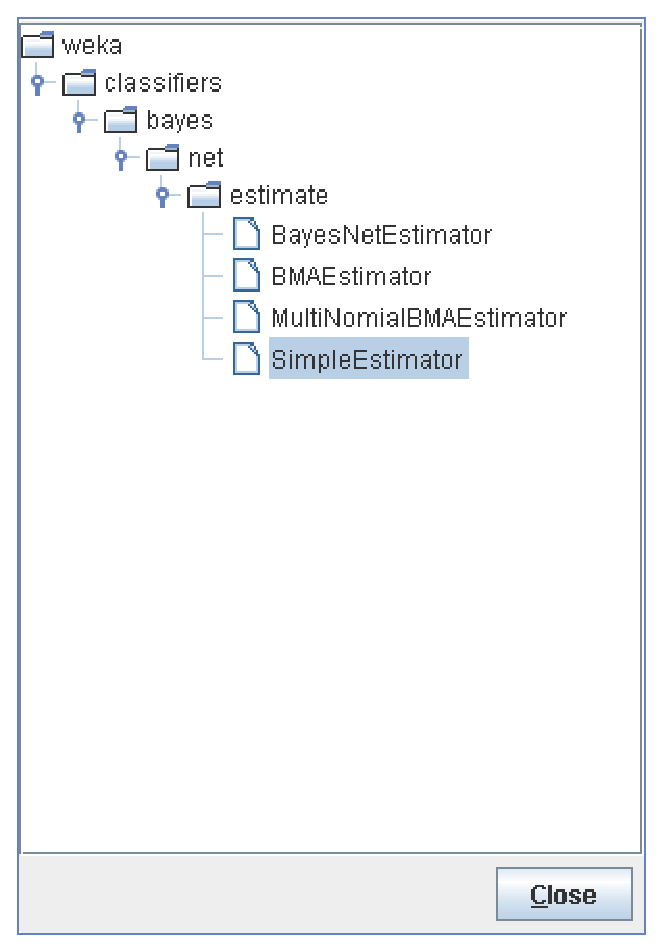
\epsfig{file=images/bayesnet/estimate.algorithms.eps,height=8cm}
\end{center}


The \texttt{SimpleEstimator} class produces direct estimates of the conditional probabilities,
that is, 
$$P(x_i=k|pa(x_i)=j)=\frac{N_{ijk}+N_{ijk}'}{N_{ij}+N_{ij}'}$$ 
where $N_{ijk}'$ is the alpha parameter that can be set and is
$0.5$ by default. With $alpha=0$, we get maximum likelihood estimates.

\begin{center}
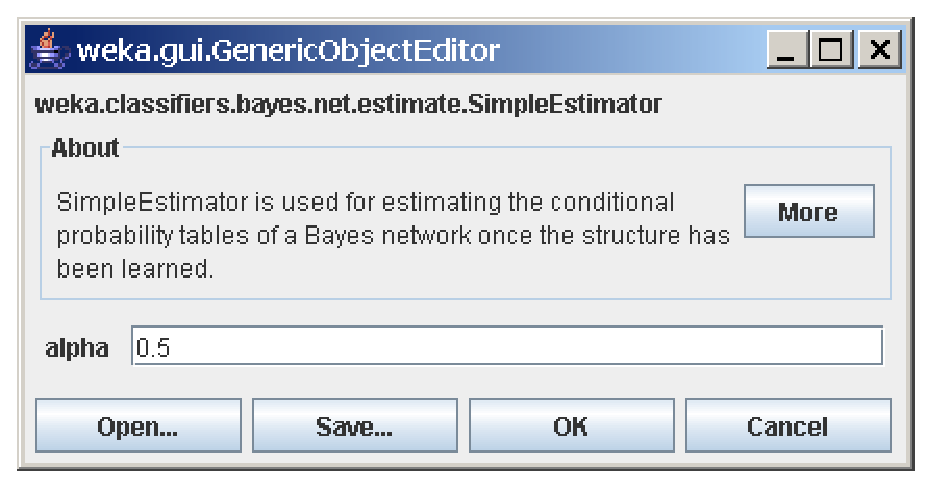
\epsfig{file=images/bayesnet/estimate.direct.eps,height=4cm}
\end{center}

With the \texttt{BMAEstimator}, we get estimates for the conditional probability tables based
on Bayes model averaging of all network structures that are substructures of the
network structure learned \cite{bouck1995}. This is achieved by estimating the
conditional probability table of a node $x_i$ given its parents $pa(x_i)$ as a weighted 
average of all conditional probability tables of $x_i$ given subsets of $pa(x_i)$.
The weight of a distribution $P(x_i|S)$ with $S\subseteq pa(x_i)$ used is proportional
to the contribution of network structure $\forall_{y\in S}y\to x_i$ to either the
BDe metric or K2 metric depending on the setting of the {\tt useK2Prior} option (\textbf{false}
and \textbf{true} respectively).

\begin{center}
\epsfig{file=images/bayesnet/estimate.bma.eps,height=5cm}
\end{center}

\section{Running from the command line}
These are the command line options of {\tt BayesNet}.

{\small
\begin{verbatim}
General options:

-t <name of training file>
        Sets training file.
-T <name of test file>
        Sets test file. If missing, a cross-validation will be performed on the 
        training data.
-c <class index>
        Sets index of class attribute (default: last).
-x <number of folds>
        Sets number of folds for cross-validation (default: 10).
-no-cv
        Do not perform any cross validation.
-split-percentage <percentage>
        Sets the percentage for the train/test set split, e.g., 66.
-preserve-order
        Preserves the order in the percentage split.
-s <random number seed>
        Sets random number seed for cross-validation or percentage split
        (default: 1).
-m <name of file with cost matrix>
        Sets file with cost matrix.
-l <name of input file>
        Sets model input file. In case the filename ends with '.xml',
        the options are loaded from the XML file.
-d <name of output file>
        Sets model output file. In case the filename ends with '.xml',
        only the options are saved to the XML file, not the model.
-v
        Outputs no statistics for training data.
-o
        Outputs statistics only, not the classifier.
-i
        Outputs detailed information-retrieval statistics for each class.
-k
        Outputs information-theoretic statistics.
-p <attribute range>
        Only outputs predictions for test instances (or the train
        instances if no test instances provided), along with attributes
        (0 for none).
-distribution
        Outputs the distribution instead of only the prediction
        in conjunction with the '-p' option (only nominal classes).
-r
        Only outputs cumulative margin distribution.
-g
        Only outputs the graph representation of the classifier.
-xml filename | xml-string
        Retrieves the options from the XML-data instead of the command line.

Options specific to weka.classifiers.bayes.BayesNet:

-D
        Do not use ADTree data structure

-B <BIF file>
        BIF file to compare with

-Q weka.classifiers.bayes.net.search.SearchAlgorithm
        Search algorithm

-E weka.classifiers.bayes.net.estimate.SimpleEstimator
        Estimator algorithm
        
\end{verbatim}
}

The search algorithm option -Q and estimator option -E options are mandatory.

Note that it is important that the -E options should be used after the
-Q option. Extra options can be passed to the search algorithm and
the estimator after the class name specified following '\texttt{--}'.

\noindent For example:
{\small
\begin{verbatim}
java weka.classifiers.bayes.BayesNet -t iris.arff -D \
  -Q weka.classifiers.bayes.net.search.local.K2 -- -P 2 -S ENTROPY \
  -E weka.classifiers.bayes.net.estimate.SimpleEstimator -- -A 1.0
\end{verbatim}
}

\subsection*{Overview of options for search algorithms}

\begin{itemize}
\item \texttt{weka.classifiers.bayes.net.search.local.GeneticSearch}
  \begin{verbatim}
-L <integer>
        Population size
-A <integer>
        Descendant population size
-U <integer>
        Number of runs
-M
        Use mutation.
        (default true)
-C
        Use cross-over.
        (default true)
-O
        Use tournament selection (true) or maximum subpopulatin (false).
        (default false)
-R <seed>
        Random number seed
-mbc
        Applies a Markov Blanket correction to the network structure,
        after a network structure is learned. This ensures that all
        nodes in the network are part of the Markov blanket of the
        classifier node.
-S [BAYES|MDL|ENTROPY|AIC|CROSS_CLASSIC|CROSS_BAYES]
        Score type (BAYES, BDeu, MDL, ENTROPY and AIC)
  \end{verbatim}
\item \texttt{weka.classifiers.bayes.net.search.local.HillClimber}
  \begin{verbatim}
-P <nr of parents>
        Maximum number of parents
-R
        Use arc reversal operation.
        (default false)
-N
        Initial structure is empty (instead of Naive Bayes)
-mbc
        Applies a Markov Blanket correction to the network structure,
        after a network structure is learned. This ensures that all
        nodes in the network are part of the Markov blanket of the
        classifier node.
-S [BAYES|MDL|ENTROPY|AIC|CROSS_CLASSIC|CROSS_BAYES]
        Score type (BAYES, BDeu, MDL, ENTROPY and AIC)
  \end{verbatim}
\item \texttt{weka.classifiers.bayes.net.search.local.K2}
  \begin{verbatim}
-N
        Initial structure is empty (instead of Naive Bayes)
-P <nr of parents>
        Maximum number of parents
-R
        Random order.
        (default false)
-mbc
        Applies a Markov Blanket correction to the network structure,
        after a network structure is learned. This ensures that all
        nodes in the network are part of the Markov blanket of the
        classifier node.
-S [BAYES|MDL|ENTROPY|AIC|CROSS_CLASSIC|CROSS_BAYES]
        Score type (BAYES, BDeu, MDL, ENTROPY and AIC)
  \end{verbatim}
\item \texttt{weka.classifiers.bayes.net.search.local.LAGDHillClimber}
  \begin{verbatim}
-L <nr of look ahead steps>
        Look Ahead Depth
-G <nr of good operations>
        Nr of Good Operations
-P <nr of parents>
        Maximum number of parents
-R
        Use arc reversal operation.
        (default false)
-N
        Initial structure is empty (instead of Naive Bayes)
-mbc
        Applies a Markov Blanket correction to the network structure,
        after a network structure is learned. This ensures that all
        nodes in the network are part of the Markov blanket of the
        classifier node.
-S [BAYES|MDL|ENTROPY|AIC|CROSS_CLASSIC|CROSS_BAYES]
        Score type (BAYES, BDeu, MDL, ENTROPY and AIC)
  \end{verbatim}
\item \texttt{weka.classifiers.bayes.net.search.local.RepeatedHillClimber}
  \begin{verbatim}
-U <integer>
        Number of runs
-A <seed>
        Random number seed
-P <nr of parents>
        Maximum number of parents
-R
        Use arc reversal operation.
        (default false)
-N
        Initial structure is empty (instead of Naive Bayes)
-mbc
        Applies a Markov Blanket correction to the network structure,
        after a network structure is learned. This ensures that all
        nodes in the network are part of the Markov blanket of the
        classifier node.
-S [BAYES|MDL|ENTROPY|AIC|CROSS_CLASSIC|CROSS_BAYES]
        Score type (BAYES, BDeu, MDL, ENTROPY and AIC)
  \end{verbatim}
\item \texttt{weka.classifiers.bayes.net.search.local.SimulatedAnnealing}
  \begin{verbatim}
-A <float>
        Start temperature
-U <integer>
        Number of runs
-D <float>
        Delta temperature
-R <seed>
        Random number seed
-mbc
        Applies a Markov Blanket correction to the network structure,
        after a network structure is learned. This ensures that all
        nodes in the network are part of the Markov blanket of the
        classifier node.
-S [BAYES|MDL|ENTROPY|AIC|CROSS_CLASSIC|CROSS_BAYES]
        Score type (BAYES, BDeu, MDL, ENTROPY and AIC)
  \end{verbatim}
\item \texttt{weka.classifiers.bayes.net.search.local.TabuSearch}
  \begin{verbatim}
-L <integer>
        Tabu list length
-U <integer>
        Number of runs
-P <nr of parents>
        Maximum number of parents
-R
        Use arc reversal operation.
        (default false)
-P <nr of parents>
        Maximum number of parents
-R
        Use arc reversal operation.
        (default false)
-N
        Initial structure is empty (instead of Naive Bayes)
-mbc
        Applies a Markov Blanket correction to the network structure,
        after a network structure is learned. This ensures that all
        nodes in the network are part of the Markov blanket of the
        classifier node.
-S [BAYES|MDL|ENTROPY|AIC|CROSS_CLASSIC|CROSS_BAYES]
        Score type (BAYES, BDeu, MDL, ENTROPY and AIC)
  \end{verbatim}
\item \texttt{weka.classifiers.bayes.net.search.local.TAN}
  \begin{verbatim}
-mbc
        Applies a Markov Blanket correction to the network structure,
        after a network structure is learned. This ensures that all
        nodes in the network are part of the Markov blanket of the
        classifier node.
-S [BAYES|MDL|ENTROPY|AIC|CROSS_CLASSIC|CROSS_BAYES]
        Score type (BAYES, BDeu, MDL, ENTROPY and AIC)
  \end{verbatim}
\item \texttt{weka.classifiers.bayes.net.search.ci.CISearchAlgorithm}
  \begin{verbatim}
-mbc
        Applies a Markov Blanket correction to the network structure,
        after a network structure is learned. This ensures that all
        nodes in the network are part of the Markov blanket of the
        classifier node.
-S [BAYES|MDL|ENTROPY|AIC|CROSS_CLASSIC|CROSS_BAYES]
        Score type (BAYES, BDeu, MDL, ENTROPY and AIC)
  \end{verbatim}
\item \texttt{weka.classifiers.bayes.net.search.ci.ICSSearchAlgorithm}
  \begin{verbatim}
-cardinality <num>
        When determining whether an edge exists a search is performed
        for a set Z that separates the nodes. MaxCardinality determines
        the maximum size of the set Z. This greatly influences the
        length of the search. (default 2)
-mbc
        Applies a Markov Blanket correction to the network structure,
        after a network structure is learned. This ensures that all
        nodes in the network are part of the Markov blanket of the
        classifier node.
-S [BAYES|MDL|ENTROPY|AIC|CROSS_CLASSIC|CROSS_BAYES]
        Score type (BAYES, BDeu, MDL, ENTROPY and AIC)
  \end{verbatim}
\item \texttt{weka.classifiers.bayes.net.search.global.GeneticSearch}
  \begin{verbatim}
-L <integer>
        Population size
-A <integer>
        Descendant population size
-U <integer>
        Number of runs
-M
        Use mutation.
        (default true)
-C
        Use cross-over.
        (default true)
-O
        Use tournament selection (true) or maximum subpopulatin (false).
        (default false)
-R <seed>
        Random number seed
-mbc
        Applies a Markov Blanket correction to the network structure,
        after a network structure is learned. This ensures that all
        nodes in the network are part of the Markov blanket of the
        classifier node.
-S [LOO-CV|k-Fold-CV|Cumulative-CV]
        Score type (LOO-CV,k-Fold-CV,Cumulative-CV)
-Q
        Use probabilistic or 0/1 scoring.
        (default probabilistic scoring)
  \end{verbatim}
\item \texttt{weka.classifiers.bayes.net.search.global.HillClimber}
  \begin{verbatim}
-P <nr of parents>
        Maximum number of parents
-R
        Use arc reversal operation.
        (default false)
-N
        Initial structure is empty (instead of Naive Bayes)
-mbc
        Applies a Markov Blanket correction to the network structure,
        after a network structure is learned. This ensures that all
        nodes in the network are part of the Markov blanket of the
        classifier node.
-S [LOO-CV|k-Fold-CV|Cumulative-CV]
        Score type (LOO-CV,k-Fold-CV,Cumulative-CV)
-Q
        Use probabilistic or 0/1 scoring.
        (default probabilistic scoring)
  \end{verbatim}
\item \texttt{weka.classifiers.bayes.net.search.global.K2}
  \begin{verbatim}
-N
        Initial structure is empty (instead of Naive Bayes)
-P <nr of parents>
        Maximum number of parents
-R
        Random order.
        (default false)
-mbc
        Applies a Markov Blanket correction to the network structure,
        after a network structure is learned. This ensures that all
        nodes in the network are part of the Markov blanket of the
        classifier node.
-S [LOO-CV|k-Fold-CV|Cumulative-CV]
        Score type (LOO-CV,k-Fold-CV,Cumulative-CV)
-Q
        Use probabilistic or 0/1 scoring.
        (default probabilistic scoring)
  \end{verbatim}
\item \texttt{weka.classifiers.bayes.net.search.global.RepeatedHillClimber}
  \begin{verbatim}
-U <integer>
        Number of runs
-A <seed>
        Random number seed
-P <nr of parents>
        Maximum number of parents
-R
        Use arc reversal operation.
        (default false)
-N
        Initial structure is empty (instead of Naive Bayes)
-mbc
        Applies a Markov Blanket correction to the network structure,
        after a network structure is learned. This ensures that all
        nodes in the network are part of the Markov blanket of the
        classifier node.
-S [LOO-CV|k-Fold-CV|Cumulative-CV]
        Score type (LOO-CV,k-Fold-CV,Cumulative-CV)
-Q
        Use probabilistic or 0/1 scoring.
        (default probabilistic scoring)
  \end{verbatim}
\item \texttt{weka.classifiers.bayes.net.search.global.SimulatedAnnealing}
  \begin{verbatim}
-A <float>
        Start temperature
-U <integer>
        Number of runs
-D <float>
        Delta temperature
-R <seed>
        Random number seed
-mbc
        Applies a Markov Blanket correction to the network structure,
        after a network structure is learned. This ensures that all
        nodes in the network are part of the Markov blanket of the
        classifier node.
-S [LOO-CV|k-Fold-CV|Cumulative-CV]
        Score type (LOO-CV,k-Fold-CV,Cumulative-CV)
-Q
        Use probabilistic or 0/1 scoring.
        (default probabilistic scoring)
  \end{verbatim}
\item \texttt{weka.classifiers.bayes.net.search.global.TabuSearch}
  \begin{verbatim}
-L <integer>
        Tabu list length
-U <integer>
        Number of runs
-P <nr of parents>
        Maximum number of parents
-R
        Use arc reversal operation.
        (default false)
-P <nr of parents>
        Maximum number of parents
-R
        Use arc reversal operation.
        (default false)
-N
        Initial structure is empty (instead of Naive Bayes)
-mbc
        Applies a Markov Blanket correction to the network structure,
        after a network structure is learned. This ensures that all
        nodes in the network are part of the Markov blanket of the
        classifier node.
-S [LOO-CV|k-Fold-CV|Cumulative-CV]
        Score type (LOO-CV,k-Fold-CV,Cumulative-CV)
-Q
        Use probabilistic or 0/1 scoring.
        (default probabilistic scoring)
  \end{verbatim}
\item \texttt{weka.classifiers.bayes.net.search.global.TAN}
  \begin{verbatim}
-mbc
        Applies a Markov Blanket correction to the network structure,
        after a network structure is learned. This ensures that all
        nodes in the network are part of the Markov blanket of the
        classifier node.
-S [LOO-CV|k-Fold-CV|Cumulative-CV]
        Score type (LOO-CV,k-Fold-CV,Cumulative-CV)
-Q
        Use probabilistic or 0/1 scoring.
        (default probabilistic scoring)
  \end{verbatim}
\item \texttt{weka.classifiers.bayes.net.search.fixed.FromFile}
  \begin{verbatim}
-B <BIF File>
        Name of file containing network structure in BIF format
  \end{verbatim}
\item \texttt{weka.classifiers.bayes.net.search.fixed.NaiveBayes}
  \begin{verbatim}
No options.
  \end{verbatim}
\end{itemize}

\subsection*{Overview of options for estimators}

\begin{itemize}
\item \texttt{weka.classifiers.bayes.net.estimate.BayesNetEstimator}
  \begin{verbatim}
-A <alpha>
        Initial count (alpha)
  \end{verbatim}
\item \texttt{weka.classifiers.bayes.net.estimate.BMAEstimator}
  \begin{verbatim}
-k2
        Whether to use K2 prior.
-A <alpha>
        Initial count (alpha)
  \end{verbatim}
\item \texttt{weka.classifiers.bayes.net.estimate.MultiNomialBMAEstimator}
  \begin{verbatim}
-k2
        Whether to use K2 prior.
-A <alpha>
        Initial count (alpha)
  \end{verbatim}
\item \texttt{weka.classifiers.bayes.net.estimate.SimpleEstimator}
  \begin{verbatim}
-A <alpha>
        Initial count (alpha)
  \end{verbatim}
\end{itemize}

\subsection*{Generating random networks and artificial data sets}

You can generate random Bayes nets and data sets using \\
\indent {\tt weka.classifiers.bayes.net.BayesNetGenerator} \\
The options are:
\begin{verbatim}
-B
        Generate network (instead of instances)
-N <integer>
        Nr of nodes
-A <integer>
        Nr of arcs
-M <integer>
        Nr of instances
-C <integer>
        Cardinality of the variables
-S <integer>
        Seed for random number generator
-F <file>
        The BIF file to obtain the structure from.
\end{verbatim}

The network structure is generated by first generating a tree so that we can
ensure that we have a connected graph. If any more arrows are specified they are
randomly added.


\section{Inspecting Bayesian networks}

You can inspect some of the properties of Bayesian networks that you learned
in the Explorer in text format and also in graphical format.
  
\subsection*{Bayesian networks in text}

Below, you find output typical for a 10 fold cross-validation run in the Weka
Explorer with comments where the output is specific for Bayesian nets. 

% iris.xml generated with:
% weka.classifiers.bayes.BayesNet -D -Q weka.classifiers.bayes.net.search.fixed.NaiveBayes -- -E weka.classifiers.bayes.net.estimate.SimpleEstimator -- -A 0.5
% and then used with:
% weka.classifiers.bayes.BayesNet -D -B iris.xml -Q weka.classifiers.bayes.net.search.local.K2 -- -P 2 -S BAYES -E weka.classifiers.bayes.net.estimate.SimpleEstimator -- -A 0.5

\begin{verbatim}
=== Run information ===

Scheme:       weka.classifiers.bayes.BayesNet -D -B iris.xml -Q weka.classifiers.bayes.net.search.local.K2 -- -P 2 -S BAYES -E weka.classifiers.bayes.net.estimate.SimpleEstimator -- -A 0.5
\end{verbatim}
Options for \texttt{BayesNet} include the class names for the structure learner and for the 
distribution estimator.
\begin{verbatim}
Relation:     iris-weka.filters.unsupervised.attribute.Discretize-B2-M-1.0-Rfirst-last
Instances:    150
Attributes:   5
              sepallength
              sepalwidth
              petallength
              petalwidth
              class
Test mode:    10-fold cross-validation

=== Classifier model (full training set) ===

Bayes Network Classifier
not using ADTree
\end{verbatim}
Indication whether the ADTree algorithm \cite{Moore} for calculating counts in the
data set was used.
\begin{verbatim}
#attributes=5 #classindex=4
\end{verbatim}
This line lists the number of attribute and the number of the class variable for which the 
classifier was trained.

\begin{verbatim}
Network structure (nodes followed by parents)
sepallength(2): class 
sepalwidth(2): class 
petallength(2): class sepallength 
petalwidth(2): class petallength 
class(3): 
\end{verbatim}
This list specifies the network structure. Each of the variables is followed by
a list of parents, so the $petallength$ variable has parents $sepallength$ and $class$,
while $class$ has no parents. The number in braces is the cardinality of the variable.
It shows that in the iris dataset there are three class variables. All other variables
are made binary by running it through a discretization filter.

\begin{verbatim}
LogScore Bayes: -374.9942769685747
LogScore BDeu: -351.85811477631626
LogScore MDL: -416.86897021246466
LogScore ENTROPY: -366.76261727150217
LogScore AIC: -386.76261727150217
\end{verbatim}
These lines list the logarithmic score of the network structure for various methods
of scoring.

If a BIF file was specified, the following two lines will be produced (if no such
file was specified, no information is printed).

\begin{verbatim}
Missing: 0 Extra: 2 Reversed: 0
Divergence: -0.0719759699700729
\end{verbatim}

In this case the network that was learned was compared with a file {\tt iris.xml}
which contained the naive Bayes network structure. The number after ``Missing''
is the number of arcs that was in the network in file that is not recovered by
the structure learner. Note that a reversed arc is not counted as missing.
The number after ``Extra'' is the number of arcs in the learned network that are
not in the network on file. The number of reversed arcs is listed as well.

Finally, the divergence between the network distribution on file and the one learned
is reported. This number is calculated by enumerating all possible instantiations
of all variables, so it may take some time to calculate the divergence for large
networks.

The remainder of the output is standard output for all classifiers. 
\begin{verbatim}
Time taken to build model: 0.01 seconds

=== Stratified cross-validation ===
=== Summary ===

Correctly Classified Instances         116               77.3333 %
Incorrectly Classified Instances        34               22.6667 %
\end{verbatim}
etc...

\subsection*{Bayesian networks in GUI}

To show the graphical structure, right click the appropriate \texttt{BayesNet} in result list of
the Explorer. A menu pops up, in which you select ``Visualize graph''.

\begin{center}
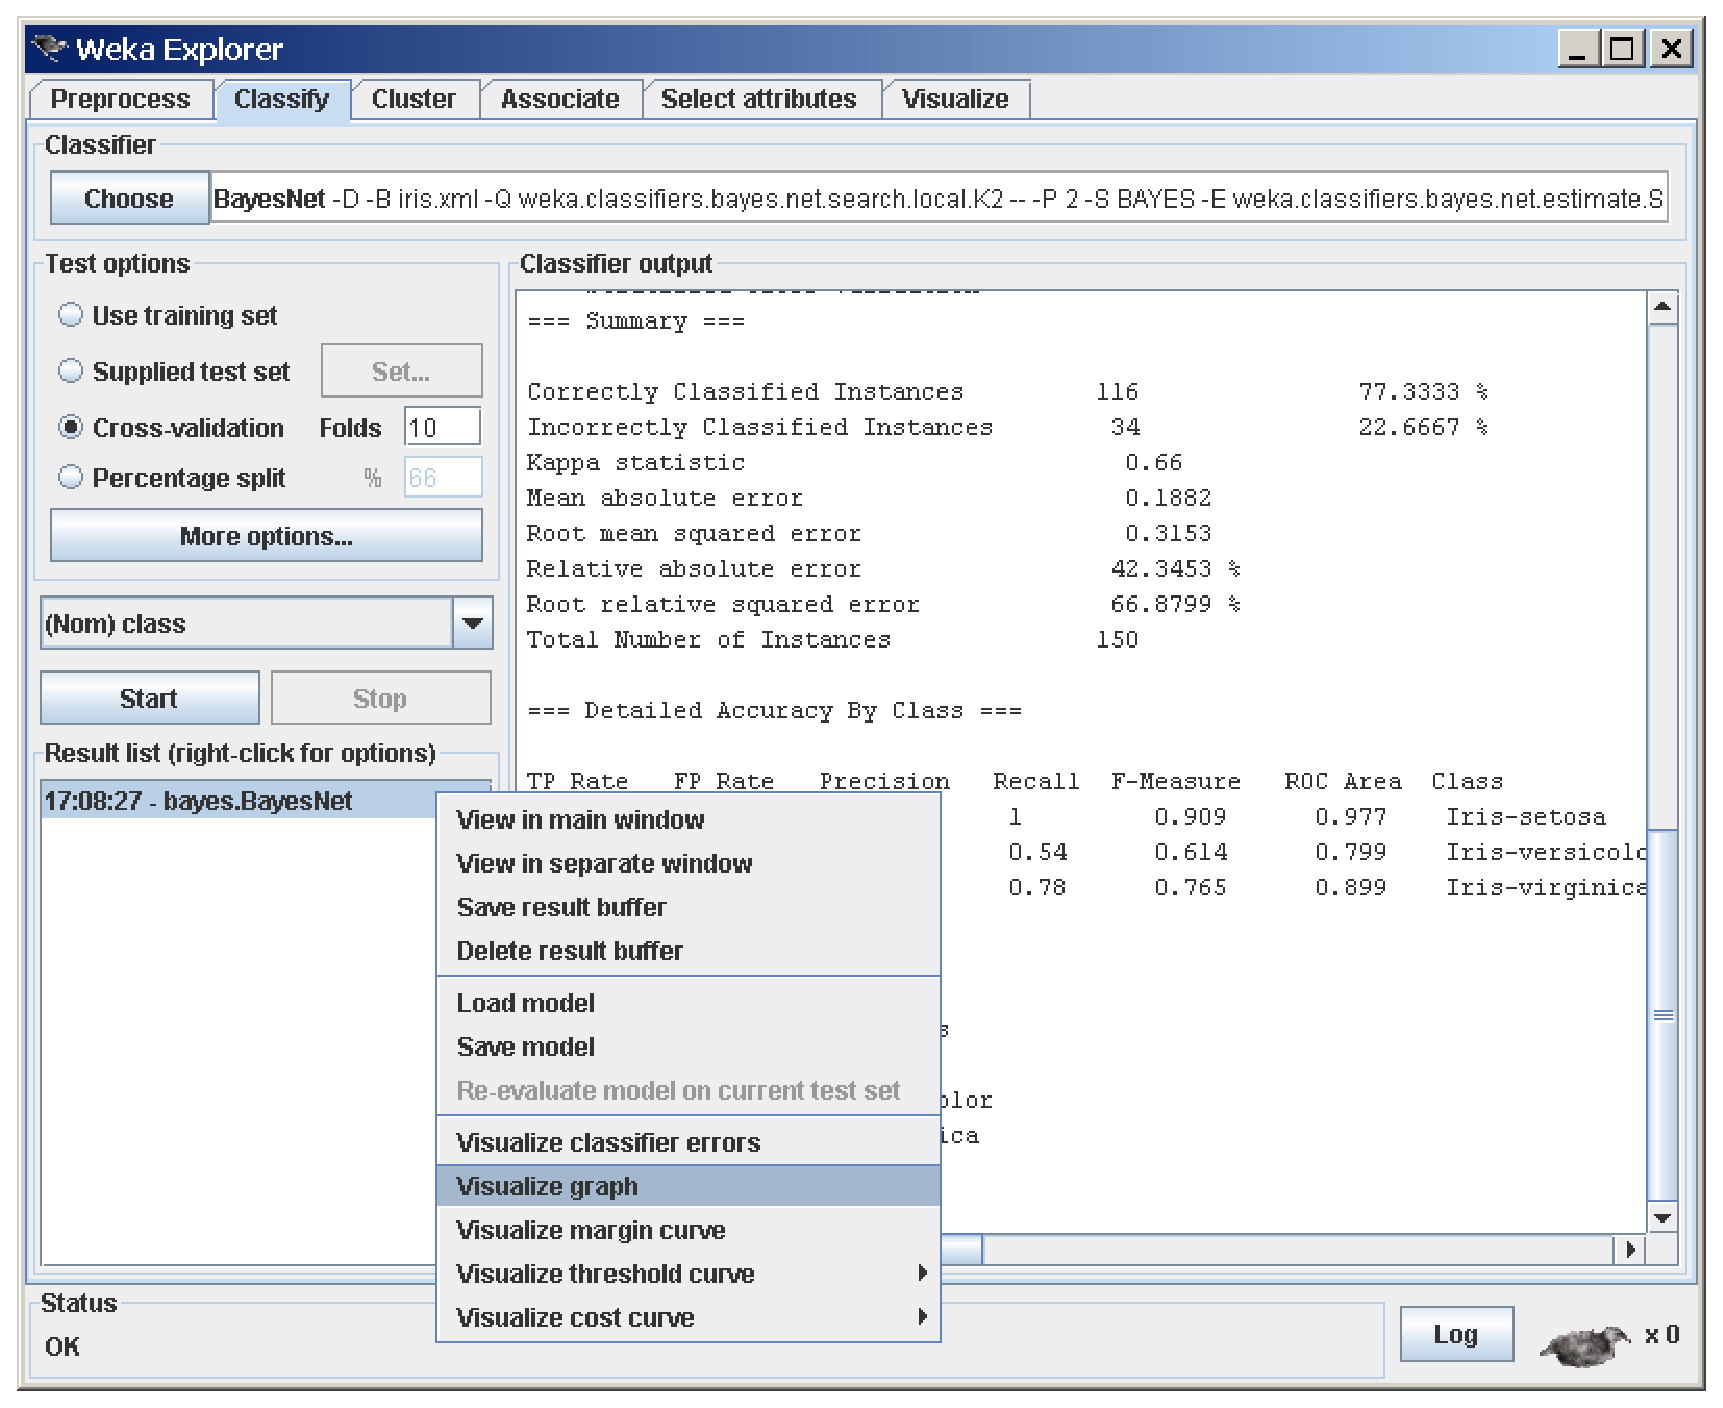
\epsfig{file=images/bayesnet/gui.select.eps,height=8cm}
\end{center}

The Bayes network is automatically layed out and drawn thanks to a graph drawing algorithm
implemented by Ashraf Kibriya.

\begin{center}
\epsfig{file=images/bayesnet/gui.net2.eps,height=7cm}
\end{center}

When you hover the mouse over a node, the node lights up and all its children are highlighted
as well, so that it is easy to identify the relation between nodes in crowded graphs.

{\bf Saving Bayes nets} You can save the Bayes network to file in the graph visualizer.
You have the choice to save as XML BIF format or as dot format. Select the floppy button
and a file save dialog pops up that allows you to select the file name and file format.

{\bf Zoom} The graph visualizer has two buttons to zoom in and out. Also, the exact zoom
desired can be entered in the zoom percentage entry. Hit enter to redraw at the desired zoom
level.

{\bf Graph drawing options} Hit the 'extra controls' button to show extra options that
control the graph layout settings.

\begin{center}
\epsfig{file=images/bayesnet/gui.netoptions.eps,height=7cm}
\end{center}

The {\tt Layout Type} determines the algorithm applied to place the nodes.

The {\tt Layout Method} determines in which direction nodes are considered.

The {\tt Edge Concentration} toggle allows edges to be partially merged.

The {\tt Custom Node Size} can be used to override the automatically determined node size.

When you click a node in the Bayesian net, a window with the probability table of the node 
clicked pops up. The left side shows the parent attributes and lists the values of the
parents, the right side shows the probability of the node clicked conditioned on the 
values of the parents listed on the left.

\begin{center}
\epsfig{file=images/bayesnet/gui.table.eps,height=3cm}
\end{center}

So, the graph visualizer allows you to inspect both network structure and probability tables. 

\section{Bayes Network GUI}

The Bayesian network editor is a stand alone application with the following features\\
$\bullet$ Edit Bayesian network completely by hand, with unlimited undo/redo stack,
cut/copy/paste and layout support.\\
$\bullet$ Learn Bayesian network from data using learning algorithms in Weka.\\
$\bullet$ Edit structure by hand and learn conditional probability tables (CPTs) using learning algorithms in Weka.\\
$\bullet$ Generate dataset from Bayesian network.\\
$\bullet$ Inference (using junction tree method) of evidence through the network,
interactively changing values of nodes.\\
$\bullet$ Viewing cliques in junction tree.\\
$\bullet$ Accelerator key support for most common operations.\\


The Bayes network GUI is started as\\
java weka.classifiers.bayes.net.GUI <bif file> \\
The following window pops up when an XML BIF file is specified (if none is
specified an empty graph is shown).

\begin{center}
\epsfig{file=images/bayesnet.editor/viewgraph.eps,height=12cm}
\end{center}


\subsubsection*{Moving a node}
Click a node with the left mouse button and drag the node to the desired position.

\subsubsection*{Selecting groups of nodes}

Drag the left mouse button in the graph panel. A rectangle is shown and
all nodes intersecting with the rectangle are selected when the mouse is
released. Selected nodes are made visible with four little black squares at the 
corners (see screenshot above).

The selection can be extended by keeping the shift key pressed while selecting
another set of nodes.

The selection can be toggled by keeping the ctrl key pressed. All nodes in the
selection selected in the rectangle are de-selected, while the ones not in the
selection but intersecting with the rectangle are added to the selection.

Groups of nodes can be moved by keeping the left mouse pressed on one of the
selected nodes and dragging the group to the desired position.

\subsubsection*{File menu}

\begin{center}
\epsfig{file=images/bayesnet.editor/menufile.eps,height=4cm}
\end{center}

The New, Save, Save As, and Exit menu provide functionality as expected.
The file format used is XML BIF \cite{cozman}.

There are two file formats supported for opening\\
$\bullet$ {\bf .xml} for XML BIF files. The Bayesian network is reconstructed
from the information in the file. Node width information is not stored so the nodes
are shown with the default width. This can be changed by laying out the graph
(menu Tools/Layout).\\
$\bullet$ {\bf .arff} Weka data files. When an arff file is selected, a new
empty Bayesian network is created with nodes for each of the attributes
in the arff file. Continuous variables are discretized using the 
{\tt weka.filters.supervised.attribute.Discretize} filter (see note at end of
this section for more details). The network
structure can be specified and the CPTs learned using the Tools/Learn CPT
menu.

The Print menu works (sometimes) as expected.

The Export menu allows for writing the graph panel to image (currently
supported are bmp, jpg, png and eps formats). This can also be activated
using the Alt-Shift-Left Click action in the graph panel.

\subsubsection*{Edit menu}

\begin{center}
\epsfig{file=images/bayesnet.editor/menuedit.eps,height=8cm}
\end{center}

Unlimited undo/redo support. Most edit operations on the Bayesian network
are undoable. A notable exception is learning of network and CPTs.

Cut/copy/paste support. When a set of nodes is selected these can be placed on
a clipboard (internal, so no interaction with other applications yet) and
a paste action will add the nodes. Nodes are renamed by adding "Copy of" before
the name and adding numbers if necessary to ensure uniqueness of name.
Only the arrows to parents are copied, not these of the children.

The Add Node menu brings up a dialog (see below) that allows to specify the name of the
new node and the cardinality of the new node. Node values are assigned the
names 'Value1', 'Value2' etc. These values can be renamed (right click the node
in the graph panel and select Rename Value). Another option is to copy/paste
a node with values that are already properly named and rename the node.

\begin{center}
\epsfig{file=images/bayesnet.editor/dlg.addnode.eps,height=2.5cm}
\end{center}

The Add Arc menu brings up a dialog to choose a child node first;

\begin{center}
\epsfig{file=images/bayesnet.editor/dlg.addarc.eps,height=2cm}
\end{center}

Then a dialog is shown to select a parent. Descendants of the child
node, parents of the child node and the node itself are not listed since
these cannot be selected as child node since they would introduce cycles
or already have an arc in the network.

\begin{center}
\epsfig{file=images/bayesnet.editor/dlg.addarc2.eps,height=2cm}
\end{center}

The Delete Arc menu brings up a dialog with a list of all arcs that
can be deleted.

\begin{center}
\epsfig{file=images/bayesnet.editor/dlg.delarc.eps,height=2cm}
\end{center}

The list of eight items at the bottom are active only when a group of at least
two nodes are selected.\\
$\bullet$ Align Left/Right/Top/Bottom moves the nodes in the selection such
that all nodes align to the utmost left, right, top or bottom node in the
selection respectively.\\
$\bullet$ Center Horizontal/Vertical moves nodes in the selection halfway
between left and right most (or top and bottom most respectively).\\
$\bullet$ Space Horizontal/Vertical spaces out nodes in the selection evenly
between left and right most (or top and bottom most respectively). The order
in which the nodes are selected impacts the place the node is moved to.\\

\subsubsection*{Tools menu}

\begin{center}
\epsfig{file=images/bayesnet.editor/menutools.eps,height=5cm}
\end{center}


The Generate Network menu allows generation of a complete random Bayesian 
network. It brings up a dialog to specify the number of nodes, number of
arcs, cardinality and a random seed to generate a network.

\begin{center}
\epsfig{file=images/bayesnet.editor/dlg.generate.eps,height=3.5cm}
\end{center}


The Generate Data menu allows for generating a data set from the Bayesian
network in the editor. A dialog is shown to specify the number of instances
to be generated, a random seed and the file to save the data set into. The
file format is arff. When no file is selected (field left blank) no file is 
written and only the internal data set is set.

\begin{center}
\epsfig{file=images/bayesnet.editor/dlg.generated.eps,height=3.5cm}
\end{center}

The Set Data menu sets the current data set. From this data set a new
Bayesian network can be learned, or the CPTs of a network can be estimated.
A file choose menu pops up to select the arff file containing the data.

The Learn Network and Learn CPT menus are only active when a data set is 
specified either through
\\$\bullet$ Tools/Set Data menu, or
\\$\bullet$ Tools/Generate Data menu, or
\\$\bullet$ File/Open menu when an arff file is selected.

The Learn Network action learns the whole Bayesian network from the data set.
The learning algorithms can be selected from the set available in Weka
by selecting the Options button in the dialog below.
Learning a network clears the undo stack.

\begin{center}
\epsfig{file=images/bayesnet.editor/dlg.learn.eps,height=2cm}
\end{center}

The Learn CPT menu does not change the structure of the Bayesian network,
only the probability tables.
Learning the CPTs clears the undo stack.

The Layout menu runs a graph layout algorithm on the network and tries to 
make the graph a bit more readable. When the menu item is selected, the node
size can be specified or left to calculate by the algorithm based on the size
of the labels by deselecting the custom node size check box.

\begin{center}
\epsfig{file=images/bayesnet.editor/dlg.layout.eps,height=3cm}
\end{center}

The Show Margins menu item makes marginal distributions visible.
These are calculated using the junction tree algorithm \cite{lauritzen}.
Marginal probabilities for nodes are shown in green next to the node.
The value of a node can be set (right click node, set evidence, select
a value) and the color is changed to red to indicate evidence is set
for the node. Rounding errors may occur in the marginal probabilities.

\begin{center}
\epsfig{file=images/bayesnet.editor/viewevidence.eps,height=8cm}
\end{center}


The Show Cliques menu item makes the cliques visible that are used
by the junction tree algorithm. Cliques are visualized using colored
undirected edges. Both margins and cliques can be shown at the same time,
but that makes for rather crowded graphs.

\begin{center}
\epsfig{file=images/bayesnet.editor/viewcliques.eps,height=8cm}
\end{center}


\subsubsection*{View menu}
The view menu allows for zooming in and out of the graph panel.
Also, it allows for hiding or showing the status and toolbars.

\begin{center}
\epsfig{file=images/bayesnet.editor/menuview.eps,height=5cm}
\end{center}

\subsubsection*{Help menu}

The help menu points to this document.

\begin{center}
\epsfig{file=images/bayesnet.editor/menuhelp.eps,height=2cm}
\end{center}


\subsubsection*{Toolbar}

\begin{center}
\epsfig{file=images/bayesnet.editor/toolbar.eps, height=0.6cm}
\end{center}

The toolbar allows a shortcut to many functions. Just hover the mouse
over the toolbar buttons and a tooltiptext pops up that tells which 
function is activated. The toolbar can be shown or hidden with the View/View 
Toolbar menu.

\subsubsection*{Statusbar}

At the bottom of the screen the statusbar shows messages. This can be 
helpful when an undo/redo action is performed that does not have any
visible effects, such as edit actions on a CPT. The statusbar can be shown 
or hidden with the View/View Statusbar menu.

\subsubsection*{Click right mouse button}

Clicking the right mouse button in the graph panel outside a node
brings up the following popup menu. It allows to add a node
at the location that was clicked, or add select a parent to
add to all nodes in the selection. If no node is selected, or no node
can be added as parent, this function is disabled.
\begin{center}
\epsfig{file=images/bayesnet.editor/popupmenuleft.eps,height=2.5cm}
\end{center}

Clicking the right mouse button on a node brings up a popup menu.

The popup menu shows list of values that can be set as evidence to selected node.
This is only visible when margins are shown (menu Tools/Show margins).
By selecting 'Clear', the value of the node is removed and the margins
calculated based on CPTs again.
\begin{center}
\epsfig{file=images/bayesnet.editor/pop.r.setevidence.eps,height=6cm}
\end{center}
	
A node can be renamed by right click and select Rename in the popup menu.
The following dialog appears that allows entering a new node name.
\begin{center}
\epsfig{file=images/bayesnet.editor/dlg.renamenode.eps,height=2.5cm}
\end{center}



The CPT of a node can be edited manually by selecting a node,
right click/Edit CPT. A dialog is shown with a table representing the
CPT. When a value is edited, the values of the remainder of the table
are update in order to ensure that the probabilities add up to 1.
It attempts to adjust the last column first, then goes backward from there.
\begin{center}
\epsfig{file=images/bayesnet.editor/dlg.CPT.eps,height=6cm}
\end{center}
The whole table can be filled with randomly generated distributions by
selecting the Randomize button.



The popup menu shows list of parents that can be added to selected node.
CPT for the node is updated by making copies for each value of the new parent.
\begin{center}
\epsfig{file=images/bayesnet.editor/pop.r.addparent.eps,height=6cm}
\end{center}

The popup menu shows list of parents that can be deleted from selected node.
CPT of the node keeps only the one conditioned on the first value of the
parent node.
\begin{center}
\epsfig{file=images/bayesnet.editor/pop.r.delparent.eps,height=6cm}
\end{center}

The popup menu shows list of children that can be deleted from selected node.
CPT of the child node keeps only the one conditioned on the first value 
of the parent node.
\begin{center}
\epsfig{file=images/bayesnet.editor/pop.r.delchild.eps,height=6cm}
\end{center}


Selecting the Add Value from the popup menu brings up this dialog,
in which the name of the new value for the node can be specified.
The distribution for the node assign zero probability to the value.
Child node CPTs are updated by copying distributions conditioned on
the new value.
\begin{center}
\epsfig{file=images/bayesnet.editor/dlg.addvalue.eps,height=2.5cm}
\end{center}

The popup menu shows list of values that can be renamed for selected node.
\begin{center}
\epsfig{file=images/bayesnet.editor/pop.r.renvalue.eps,height=6cm}
\end{center}

Selecting a value brings up the following dialog in which a new name
can be specified.
\begin{center}
\epsfig{file=images/bayesnet.editor/dlg.renamevalue.eps,height=2.5cm}
\end{center}

The popup menu shows list of values that can be deleted from selected node.
This is only active when there are more then two values for the node (single
valued nodes do not make much sense).
By selecting the value the CPT of the node is updated in order to ensure
that the CPT adds up to unity. The CPTs of children are updated by dropping
the distributions conditioned on the value.
\begin{center}
\epsfig{file=images/bayesnet.editor/pop.r.delvalue.eps,height=6cm}
\end{center}


\subsection*{A note on CPT learning}

Continuous variables are discretized by the Bayes network class.
The discretization algorithm chooses its values based on the information
in the data set. However, these values are not stored anywhere. So,
reading an arff file with continuous variables using the File/Open menu
allows one to specify a network, then learn the CPTs from it since the
discretization bounds are still known. However, opening an arff file, specifying
a structure, then closing the application, reopening and trying to learn the
network from another file containing continuous variables may not give the
desired result since a the discretization algorithm is re-applied and new
boundaries may have been found. Unexpected behavior may be the result.

Learning from a dataset that contains more attributes than there are nodes
in the network is ok. The extra attributes are just ignored.

Learning from a dataset with differently ordered attributes is ok. Attributes
are matched to nodes based on name. However, attribute values are matched
with node values based on the order of the values.

The attributes in the dataset should have the same number of values as the
corresponding nodes in the network (see above for continuous variables).

\section{Bayesian nets in the experimenter}

Bayesian networks generate extra measures that can be examined in the experimenter.
The experimenter can then be used to calculate mean and variance for those measures.

The following metrics are generated:
\begin{itemize}
\item measureExtraArcs: extra arcs compared to reference network. The network must be
provided as BIFFile to the BayesNet class. If no such network is provided, this value is zero.
\item measureMissingArcs: missing arcs compared to reference network or zero if not provided.
\item measureReversedArcs: reversed arcs compared to reference network or zero if not provided.
\item measureDivergence: divergence of network learned compared to reference network or zero if not provided.
\item measureBayesScore: log of the K2 score of the network structure.
\item measureBDeuScore: log of the BDeu score of the network structure.
\item measureMDLScore: log of the MDL score.
\item measureAICScore: log of the AIC score.
\item measureEntropyScore:log of the entropy.
\end{itemize}


\section{Adding your own Bayesian network learners}

You can add your own structure learners and estimators.

\subsection*{Adding a new structure learner}

Here is the quick guide for adding a structure learner:

\begin{enumerate}
\item Create a class that derives from {\tt weka.classifiers.bayes.net.search.SearchAlgorithm}.
  If your searcher is score based, conditional independence based or cross-validation based, you
  probably want to derive from {\tt ScoreSearchAlgorithm}, {\tt CISearchAlgorithm} or {\tt CVSearchAlgorithm}
  instead of deriving from {\tt SearchAlgorithm} directly.
  Let's say it is called \\{\tt weka.classifiers.bayes.net.search.local.MySearcher}
  derived from {\tt ScoreSearchAlgorithm}.

\item Implement the method\\
{\tt public void buildStructure(BayesNet bayesNet, Instances instances)}.
Essentially, you are responsible for setting the parent sets in {\tt bayesNet}.
You can access the parentsets using {\tt bayesNet.getParentSet(iAttribute)} where
{\tt iAttribute} is the number of the node/variable.

To add a parent {\tt iParent} to node {\tt iAttribute}, use\\ 
{\tt bayesNet.getParentSet(iAttribute).AddParent(iParent, instances)} where
{\tt instances} need to be passed for the parent set to derive properties of
the attribute.

Alternatively, implement
{\tt public void search(BayesNet bayesNet, Instances instances)}.
The implementation of {\tt buildStructure} in the base class.
This method is called by the {\tt SearchAlgorithm} will call search
after initializing parent sets and if the {\tt initAsNaiveBase} flag is set, it will
start with a naive Bayes network structure. After calling {\tt search} in your
custom class, it will add arrows if the {\tt markovBlanketClassifier} flag is 
set to ensure all attributes are in the Markov blanket of the class node.

\item If the structure learner has options that are not default options,
you want to implement {\tt public Enumeration listOptions()}, 
{\tt public void setOptions(String[] options)}, 
{\tt public String[] getOptions()} and the get and set methods for
the properties you want to be able to set.

NB 1. do not use the -E option since that is reserved for the {\tt BayesNet} class to 
distinguish the extra options for the {\tt SearchAlgorithm} class and the {\tt Estimator} class.
If the -E option is used, it will not be passed to your {\tt SearchAlgorithm} (and
probably causes problems in the {\tt BayesNet} class).

NB 2. make sure to process options of the parent class if any in the get/setOpions
methods.
\end{enumerate}

\subsection*{Adding a new estimator}

This is the quick guide for adding a new estimator:

\begin{enumerate}
\item Create a class that derives from \\
  {\tt weka.classifiers.bayes.net.estimate.BayesNetEstimator}.
  Let's say it is called \\
  {\tt weka.classifiers.bayes.net.estimate.MyEstimator}.

\item Implement the methods\\
{\tt public void initCPTs(BayesNet bayesNet)} \\
{\tt public void estimateCPTs(BayesNet bayesNet)} \\
{\tt public void updateClassifier(BayesNet bayesNet, Instance instance)}, and \\
{\tt  public double[] distributionForInstance(BayesNet bayesNet, Instance instance)}.

\item If the structure learner has options that are not default options,
you want to implement {\tt public Enumeration listOptions()},
{\tt public void setOptions(String[] options)},
{\tt public String[] getOptions()} and the get and set methods for
the properties you want to be able to set.

NB do not use the -E option since that is reserved for the BayesNet class to 
distinguish the extra options for the SearchAlgorithm class and the Estimator class.
If the -E option is used and no extra arguments are passed to the SearchAlgorithm,
the extra options to your Estimator will be passed to the SearchAlgorithm
instead. In short, do not use the -E option.
\end{enumerate}

\section{FAQ}

\subsection*{How do I use a data set with continuous variables with the BayesNet classes?}
Use the class {\tt weka.filters.unsupervised.attribute.Discretize} to discretize them.
From the command line, you can use\\
{\tt java weka.filters.unsupervised.attribute.Discretize -B 3 -i infile.arff -o outfile.arff}\\
where the -B option determines the cardinality of the discretized variables.

\subsection*{How do I use a data set with missing values with the BayesNet classes?}
You would have to delete the entries with missing values or
fill in dummy values.

\subsection*{How do I create a random Bayes net structure?}

Running from the command line \\
{\tt java  weka.classifiers.bayes.net.BayesNetGenerator -B -N 10 -A 9 -C 2}\\
will print a Bayes net with 10 nodes, 9 arcs and binary variables
in XML BIF format to standard output.

\subsection*{How do I create an artificial data set using a random Bayes nets?}
Running\\
{\tt java  weka.classifiers.bayes.net.BayesNetGenerator -N 15 -A 20 -C 3 -M 300}\\
will generate a data set in arff format with 300 instance from a random
network with 15 ternary variables and 20 arrows.

\subsection*{How do I create an artificial data set using a Bayes nets I have on file?}
Running\\
{\tt java  weka.classifiers.bayes.net.BayesNetGenerator -F alarm.xml -M 1000}\\
will generate a data set with 1000 instances from the network stored in the file
{\tt alarm.xml}.

\subsection*{How do I save a Bayes net in BIF format?}
\begin{itemize}
\item {\bf GUI:} In the Explorer
\begin{itemize}
\item learn the network structure,
\item right click the relevant run in the result list,
\item choose ``Visualize graph'' in the pop up menu,
\item click the floppy button in the Graph Visualizer window.
\item a file ``save as'' dialog pops up that allows you to select the file name to save to.
\end{itemize}

\item {\bf Java:} Create a {\tt BayesNet} and call {\tt BayesNet.toXMLBIF03()}
which returns the Bayes network in BIF format as a String.

\item {\bf Command line:} use the {\tt -g} option and redirect the output on stdout into a file.
\end{itemize}

\subsection*{How do I compare a network I learned with one in BIF format?}
Specify the -B $<$bif-file$>$ option to BayesNet. 
Calling {\tt toString()} will produce a summary of extra, missing and reversed arrows.
Also the divergence between the network learned and the one on file is reported.

\subsection*{How do I use the network I learned for general inference?}
There is no general purpose inference in Weka, but you can export the
network as XML BIF file (see above) and import it in other packages,
for example JavaBayes available under GPL from
\url{http://www.cs.cmu.edu/\~javabayes}{}.


\section{Future development}

If you would like to add to the current Bayes network facilities in Weka, you might
consider one of the following possibilities.

\begin{itemize}
\item Implement more search algorithms, in particular, 
\begin{itemize}
\item general purpose search algorithms (such as an improved implementation of 
genetic search).
\item structure search based on equivalent model classes.
\item implement those algorithms both for local and global metric based search algorithms.
\item implement more conditional independence based search algorithms.
\end{itemize}

\item Implement score metrics that can handle sparse instances in order to allow 
for processing large datasets.

\item Implement traditional conditional independence tests for conditional
independence based structure learning algorithms.

\item Currently, all search algorithms assume that all variables are discrete.
Search algorithms that can handle continuous variables would be interesting.

\item A limitation of the current classes is that they assume that there
are no missing values. This limitation can be undone by implementing score metrics 
that can handle missing values.
The classes used for estimating the conditional probabilities need to be updated
as well.

\item Only leave-one-out, k-fold and cumulative cross-validation are implemented.
These implementations can be made more efficient and other cross-validation methods
can be implemented, such as Monte Carlo cross-validation and bootstrap cross
validation.

\item Implement methods that can handle incremental extensions of the data set for
updating network structures.

\end{itemize}

And for the more ambitious people, there are the following challenges.

\begin{itemize}
\item A GUI for manipulating Bayesian network to allow user intervention for
adding and deleting arcs and updating the probability tables.

\item General purpose inference algorithms built into the GUI to allow user
defined queries.

\item Allow learning of other graphical models, such as chain graphs,
undirected graphs and variants of causal graphs.

\item Allow learning of networks with latent variables.

\item Allow learning of dynamic Bayesian networks so that time series data
can be handled.
\end{itemize}


%%%%%%%%%%%%%%%%%%%%%%%%%%%%%%%%%%%
\part{Data}

\chapter{ARFF}
% Version: $Revision$

An ARFF (= \textit{Attribute-Relation File Format}) file is an ASCII text file that describes a list of instances sharing a set of attributes.

\section{Overview}
ARFF files have two distinct sections. The first section is the \textbf{Header} information, which is followed the \textbf{Data} information.

The \textbf{Header} of the ARFF file contains the name of the relation, a list of the attributes (the columns in the data), and their types. An example header on the standard IRIS dataset looks like this:

\begin{verbatim}
  % 1. Title: Iris Plants Database
  % 
  % 2. Sources:
  %      (a) Creator: R.A. Fisher
  %      (b) Donor: Michael Marshall (MARSHALL%PLU@io.arc.nasa.gov)
  %      (c) Date: July, 1988
  % 
  @RELATION iris

  @ATTRIBUTE sepallength  NUMERIC
  @ATTRIBUTE sepalwidth   NUMERIC
  @ATTRIBUTE petallength  NUMERIC
  @ATTRIBUTE petalwidth   NUMERIC
  @ATTRIBUTE class        {Iris-setosa,Iris-versicolor,Iris-virginica}
\end{verbatim}

\noindent The \textbf{Data} of the ARFF file looks like the following:

\begin{verbatim}
  @DATA
  5.1,3.5,1.4,0.2,Iris-setosa
  4.9,3.0,1.4,0.2,Iris-setosa
  4.7,3.2,1.3,0.2,Iris-setosa
  4.6,3.1,1.5,0.2,Iris-setosa
  5.0,3.6,1.4,0.2,Iris-setosa
  5.4,3.9,1.7,0.4,Iris-setosa
  4.6,3.4,1.4,0.3,Iris-setosa
  5.0,3.4,1.5,0.2,Iris-setosa
  4.4,2.9,1.4,0.2,Iris-setosa
  4.9,3.1,1.5,0.1,Iris-setosa
\end{verbatim}

Lines that begin with a \texttt{\%} are comments. The \texttt{@RELATION}, \texttt{@ATTRIBUTE} and \texttt{@DATA} declarations are case insensitive.


\section{Examples}
Several well-known machine learning datasets are distributed with Weka in the \texttt{\$WEKAHOME/data} directory as ARFF files.


\subsection{The ARFF Header Section}
The ARFF Header section of the file contains the relation declaration and attribute declarations. 


\subsubsection*{The @relation Declaration}
The relation name is defined as the first line in the ARFF file. The format is:

\begin{verbatim}
  @relation <relation-name>
\end{verbatim}

where \textit{$<$relation-name$>$} is a string. The string must be quoted if the name includes spaces.


\subsubsection*{The @attribute Declarations}
Attribute declarations take the form of an ordered sequence of \texttt{@attribute} statements. Each attribute in the data set has its own \texttt{@attribute} statement which uniquely defines the name of that attribute and it's data type. The order the attributes are declared indicates the column position in the data section of the file. For example, if an attribute is the third one declared then Weka expects that all that attributes values will be found in the third comma delimited column.

The format for the \texttt{@attribute} statement is:

\begin{verbatim}
  @attribute <attribute-name> <datatype>
\end{verbatim}

where the \textit{$<$attribute-name$>$} must start with an alphabetic character. If spaces are to be included in the name then the entire name must be quoted.

The \textit{$<$datatype$>$} can be any of the four types supported by Weka:
\begin{itemize}
	\item \textit{numeric}
	\item \textit{integer} is treated as \textit{numeric}
	\item \textit{real} is treated as \textit{numeric}
	\item $<$nominal-specification$>$
	\item \textit{string}
	\item \textit{date} [$<$date-format$>$]
	\item \textit{relational} for multi-instance data (for future use)
\end{itemize}

where \textit{$<$nominal-specification$>$} and \textit{$<$date-format$>$} are defined below. The keywords \textbf{numeric}, \textbf{real}, \textbf{integer}, \textbf{string} and \textbf{date} are case insensitive.


\subsubsection*{Numeric attributes}
Numeric attributes can be real or integer numbers. 


\subsubsection*{Nominal attributes}
Nominal values are defined by providing an $<$nominal-specification$>$ listing the possible values: \texttt{{$<$nominal-name1$>$, $<$nominal-name2$>$, $<$nominal-name3$>$, ...}}

For example, the class value of the Iris dataset can be defined as follows:

\begin{verbatim}
  @ATTRIBUTE class {Iris-setosa,Iris-versicolor,Iris-virginica}
\end{verbatim}

Values that contain spaces must be quoted. 


\subsubsection*{String attributes}
String attributes allow us to create attributes containing arbitrary textual values. This is very useful in text-mining applications, as we can create datasets with string attributes, then write Weka Filters to manipulate strings (like StringToWordVectorFilter). String attributes are declared as follows:

\begin{verbatim}
  @ATTRIBUTE LCC string
\end{verbatim}


\subsubsection*{Date attributes}
Date attribute declarations take the form:

\begin{verbatim}
  @attribute <name> date [<date-format>]
\end{verbatim}

where \textit{$<$name$>$} is the name for the attribute and \textit{$<$date-format$>$} is an optional string specifying how date values should be parsed and printed (this is the same format used by \texttt{SimpleDateFormat}). The default format string accepts the ISO-8601 combined date and time format: \texttt{yyyy-MM-dd'T'HH:mm:ss}.

Dates must be specified in the data section as the corresponding string representations of the date/time (see example below). 

\subsubsection*{Relational attributes}
Relational attribute declarations take the form:

\begin{verbatim}
  @attribute <name> relational
    <further attribute definitions>
  @end <name>
\end{verbatim}

\noindent For the multi-instance dataset MUSK1 the definition would look like this ("..." denotes an omission):

\begin{verbatim}
  @attribute molecule_name {MUSK-jf78,...,NON-MUSK-199}
  @attribute bag relational
    @attribute f1 numeric
    ...
    @attribute f166 numeric
  @end bag
  @attribute class {0,1}
  ...
\end{verbatim}


\subsection{The ARFF Data Section}
The ARFF Data section of the file contains the data declaration line and the actual instance lines.


\subsubsection*{The @data Declaration}
The \texttt{@data} declaration is a single line denoting the start of the data segment in the file. The format is:

\begin{verbatim}
  @data
\end{verbatim}


\subsubsection*{The instance data}
Each instance is represented on a single line, with carriage returns denoting the end of the instance. A percent sign (\texttt{\%}) introduces a comment, which continues to the end of the line.

Attribute values for each instance are delimited by commas. They must appear in the order that they were declared in the header section (i.e. the data corresponding to the nth \texttt{@attribute} declaration is always the nth field of the attribute).

Missing values are represented by a single question mark, as in:

\begin{verbatim}
  @data
  4.4,?,1.5,?,Iris-setosa
\end{verbatim}

\noindent Values of string and nominal attributes are case sensitive, and any that contain space or the comment-delimiter character \texttt{\%} must be quoted. (The code suggests that double-quotes are acceptable and that a backslash will escape individual characters.) An example follows:

\begin{verbatim}
  @relation LCCvsLCSH

  @attribute LCC string
  @attribute LCSH string

  @data
  AG5,   'Encyclopedias and dictionaries.;Twentieth century.'
  AS262, 'Science -- Soviet Union -- History.'
  AE5,   'Encyclopedias and dictionaries.'
  AS281, 'Astronomy, Assyro-Babylonian.;Moon -- Phases.'
  AS281, 'Astronomy, Assyro-Babylonian.;Moon -- Tables.'
\end{verbatim}

\noindent Dates must be specified in the data section using the string representation specified in the attribute declaration. For example:

\begin{verbatim}
  @RELATION Timestamps

  @ATTRIBUTE timestamp DATE "yyyy-MM-dd HH:mm:ss"

  @DATA
  "2001-04-03 12:12:12"
  "2001-05-03 12:59:55"
\end{verbatim}

\noindent Relational data must be enclosed within double quotes ". For example an instance of the MUSK1 dataset ("..." denotes an omission):

\begin{verbatim}
  MUSK-188,"42,...,30",1
\end{verbatim}


\section{Sparse ARFF files}
Sparse ARFF files are very similar to ARFF files, but data with value 0 are not be explicitly represented.

Sparse ARFF files have the same header (i.e \texttt{@relation} and \texttt{@attribute} tags) but the data section is different. Instead of representing each value in order, like this:

\begin{verbatim}
  @data
  0, X, 0, Y, "class A"
  0, 0, W, 0, "class B"
\end{verbatim}

\noindent the non-zero attributes are explicitly identified by attribute number and their value stated, like this:

\begin{verbatim}
  @data
  {1 X, 3 Y, 4 "class A"}
  {2 W, 4 "class B"}
\end{verbatim}

\noindent Each instance is surrounded by curly braces, and the format for each entry is: $<$index$>$ $<$space$>$ $<$value$>$ where index is the attribute index (starting from 0).

Note that the omitted values in a sparse instance are \textbf{0}, they are not \textbf{missing} values! If a value is unknown, you must explicitly represent it with a question mark (\texttt{?}).

\textbf{Warning:} There is a known problem saving \texttt{SparseInstance} objects from datasets that have string attributes. In Weka, string and nominal data values are stored as numbers; these numbers act as indexes into an array of possible attribute values (this is very efficient). However, the first string value is assigned index 0: this means that, internally, this value is stored as a 0. When a \texttt{SparseInstance} is written, string instances with internal value 0 are not output, so their string value is lost (and when the arff file is read again, the default value 0 is the index of a different string value, so the attribute value appears to change). To get around this problem, add a dummy string value at index 0 that is never used whenever you declare string attributes that are likely to be used in \texttt{SparseInstance} objects and saved as Sparse ARFF files.

\section{Instance weights in ARFF files}
A weight can be associated with an instance in a standard ARFF file by appending it to the end of the line for that instance and enclosing the value in curly braces. E.g:

\begin{verbatim}
  @data
  0, X, 0, Y, "class A", {5}
\end{verbatim}

\noindent For a sparse instance, this example would look like:

\begin{verbatim}
  @data
  {1 X, 3 Y, 4 "class A"}, {5}
\end{verbatim}

\noindent Note that any instance without a weight value specified is assumed to have a weight of 1 for backwards compatibility.


\chapter{XRFF}
\label{xrff}
%
%   This program is free software: you can redistribute it and/or modify
%   it under the terms of the GNU General Public License as published by
%   the Free Software Foundation, either version 3 of the License, or
%   (at your option) any later version.
%
%   This program is distributed in the hope that it will be useful,
%   but WITHOUT ANY WARRANTY; without even the implied warranty of
%   MERCHANTABILITY or FITNESS FOR A PARTICULAR PURPOSE.  See the
%   GNU General Public License for more details.
%
%   You should have received a copy of the GNU General Public License
%   along with this program.  If not, see <http://www.gnu.org/licenses/>.
%

% Version: $Revision$

The XRFF (\textit{Xml attribute Relation File Format}) is a representing
the data in a format that can store comments, attribute and instance weights.

\section{File extensions}
The following file extensions are recognized as XRFF files:

\begin{itemize}
	\item \texttt{.xrff} \\
		the default extension of XRFF files
	\item \texttt{.xrff.gz} \\
		the extension for gzip compressed XRFF files (see \textit{Compression} section for more details)
\end{itemize}

\section{Comparison}

\subsection{ARFF}
In the following a snippet of the UCI dataset \textit{iris} in ARFF format:

\begin{verbatim}
  @relation iris

  @attribute sepallength numeric
  @attribute sepalwidth numeric
  @attribute petallength numeric
  @attribute petalwidth numeric
  @attribute class {Iris-setosa,Iris-versicolor,Iris-virginica}

  @data
  5.1,3.5,1.4,0.2,Iris-setosa
  4.9,3,1.4,0.2,Iris-setosa
  ...
\end{verbatim}

\subsection{XRFF}
And the same dataset represented as XRFF file:

\begin{verbatim}
  <?xml version="1.0" encoding="utf-8"?>

  <!DOCTYPE dataset
  [
     <!ELEMENT dataset (header,body)>
     <!ATTLIST dataset name CDATA #REQUIRED>
     <!ATTLIST dataset version CDATA "3.5.4">

     <!ELEMENT header (notes?,attributes)>
     <!ELEMENT body (instances)>
     <!ELEMENT notes ANY>   

     <!ELEMENT attributes (attribute+)>
     <!ELEMENT attribute (labels?,metadata?,attributes?)>
     <!ATTLIST attribute name CDATA #REQUIRED>
     <!ATTLIST attribute type (numeric|date|nominal|string|relational) #REQUIRED>
     <!ATTLIST attribute format CDATA #IMPLIED>
     <!ATTLIST attribute class (yes|no) "no">
     <!ELEMENT labels (label*)>   
     <!ELEMENT label ANY>
     <!ELEMENT metadata (property*)>
     <!ELEMENT property ANY>
     <!ATTLIST property name CDATA #REQUIRED>

     <!ELEMENT instances (instance*)>
     <!ELEMENT instance (value*)>
     <!ATTLIST instance type (normal|sparse) "normal">
     <!ATTLIST instance weight CDATA #IMPLIED>
     <!ELEMENT value (#PCDATA|instances)*>
     <!ATTLIST value index CDATA #IMPLIED>   
     <!ATTLIST value missing (yes|no) "no">
  ]
  >

  <dataset name="iris" version="3.5.3">
     <header>
        <attributes>
           <attribute name="sepallength" type="numeric"/>
           <attribute name="sepalwidth" type="numeric"/>
           <attribute name="petallength" type="numeric"/>
           <attribute name="petalwidth" type="numeric"/>
           <attribute class="yes" name="class" type="nominal">
              <labels>
                 <label>Iris-setosa</label>
                 <label>Iris-versicolor</label>
                 <label>Iris-virginica</label>
              </labels>
           </attribute>
        </attributes>
     </header>

     <body>
        <instances>
           <instance>
              <value>5.1</value>
              <value>3.5</value>
              <value>1.4</value>
              <value>0.2</value>
              <value>Iris-setosa</value>
           </instance>
           <instance>
              <value>4.9</value>
              <value>3</value>
              <value>1.4</value>
              <value>0.2</value>
              <value>Iris-setosa</value>
           </instance>
           ...
        </instances>
     </body>
  </dataset>
\end{verbatim}

\section{Sparse format}
The XRFF format also supports a sparse data representation. Even though the iris dataset does not contain sparse data, the above example will be used here to illustrate the sparse format:

\begin{verbatim}
  ...
  <instances>
     <instance type="sparse">
        <value index="1">5.1</value>
        <value index="2">3.5</value>
        <value index="3">1.4</value>
        <value index="4">0.2</value>
        <value index="5">Iris-setosa</value>
     </instance>
     <instance type="sparse">
        <value index="1">4.9</value>
        <value index="2">3</value>
        <value index="3">1.4</value>
        <value index="4">0.2</value>
        <value index="5">Iris-setosa</value>
     </instance>
     ...
  </instances>
  ...
\end{verbatim}

\noindent In contrast to the \textit{normal} data format, each sparse instance tag contains a type attribute with the value sparse:

\begin{verbatim}
  <instance type="sparse">
\end{verbatim}

\noindent And each value tag needs to specify the \textit{index} attribute, which contains the 1-based index of this value.

\begin{verbatim}
  <value index="1">5.1</value>
\end{verbatim}

\section{Compression}
Since the XML representation takes up considerably more space than the rather compact ARFF format, one can also compress the data via \textbf{gzip}. Weka automatically recognizes a file being gzip compressed, if the file's extension is \texttt{.xrff.gz} instead of \texttt{.xrff}.

The Weka Explorer, Experimenter and command-line allow one to load/save compressed and uncompressed XRFF files (this applies also to ARFF files).

\section{Useful features}
In addition to all the features of the ARFF format, the XRFF format contains the following additional features:

\begin{itemize}
	\item class attribute specification
	\item attribute weights
\end{itemize}

\subsection{Class attribute specification}
Via the \texttt{class="yes"} attribute in the attribute specification in the header, one can define which attribute should act as class attribute. A feature that can be used on the command line as well as in the Experimenter, which now can also load other data formats, and removing the limitation of the class attribute always having to be the last one.

Snippet from the \textit{iris} dataset:

\begin{verbatim}
  <attribute class="yes" name="class" type="nominal">
\end{verbatim}

\subsection{Attribute weights}
Attribute weights are stored in an attributes meta-data tag (in the \textit{header} section). Here is an example of the \textit{petalwidth} attribute with a weight of 0.9:

\begin{verbatim}
  <attribute name="petalwidth" type="numeric">
      <metadata>
         <property name="weight">0.9</property>
      </metadata>
  </attribute>
\end{verbatim}

\subsection{Instance weights}
Instance weights are defined via the \textit{weight} attribute in each instance tag. By default, the weight is 1. Here is an example:

\begin{verbatim}
  <instance weight="0.75">
     <value>5.1</value>
     <value>3.5</value>
     <value>1.4</value>
     <value>0.2</value>
     <value>Iris-setosa</value>
  </instance>
\end{verbatim}


\chapter{Converters}
%
%   This program is free software: you can redistribute it and/or modify
%   it under the terms of the GNU General Public License as published by
%   the Free Software Foundation, either version 3 of the License, or
%   (at your option) any later version.
%
%   This program is distributed in the hope that it will be useful,
%   but WITHOUT ANY WARRANTY; without even the implied warranty of
%   MERCHANTABILITY or FITNESS FOR A PARTICULAR PURPOSE.  See the
%   GNU General Public License for more details.
%
%   You should have received a copy of the GNU General Public License
%   along with this program.  If not, see <http://www.gnu.org/licenses/>.
%

% Version: $Revision$

\section{Introduction}
Weka offers conversion utilities for several formats, in order to allow import from different sorts of datasources. These utilities, called converters, are all located in the following package:

\begin{verbatim}
  weka.core.converters
\end{verbatim}

\noindent For a certain kind of converter you will find two classes

\begin{itemize}
	\item one for \textbf{loading} (classname ends with \textit{Loader}) and
	\item one for \textbf{saving} (classname ends with \textit{Saver}).
\end{itemize}

\noindent Weka contains converters for the following data sources:

\begin{itemize}
	\item \textbf{ARFF} files (ArffLoader, ArffSaver)
	\item \textbf{C4.5} files (C45Loader, C45Saver)
	\item \textbf{CSV} files (CSVLoader, CSVSaver)
	\item files containing \textbf{serialized instances} (SerializedInstancesLoader, SerializedInstancesSaver)
	\item JDBC \textbf{databases} (DatabaseLoader, DatabaseSaver)
	\item \textbf{libsvm} files (LibSVMLoader, LibSVMSaver)
	\item \textbf{XRFF} files (XRFFLoader, XRFFSaver)
	\item \textbf{text directories} for text mining (TextDirectoryLoader)
\end{itemize}

\section{Usage}

\subsection{File converters}
File converters can be used as follows:

\begin{itemize}
	\item \textbf{Loader} \\
		They take one argument, which is the file that should be converted, and print the result to stdout. You can also redirect the output into a file:
		\begin{verbatim}
 		  java <classname> <input-file> > <output-file>
		\end{verbatim}
		\noindent Here's an example for loading the CSV file \textit{iris.csv} and saving it as \textit{iris.arff}:
		\begin{verbatim}
 		  java weka.core.converters.CSVLoader iris.csv > iris.arff
		\end{verbatim}

	\item \textbf{Saver} \\
		For a Saver you specify the ARFF input file via \textit{-i} and the output file in the specific format with \textit{-o}:
		\begin{verbatim}
		  java <classname> -i <input> -o <output>
		\end{verbatim}
		\noindent Here's an example for saving an ARFF file to CSV:
		\begin{verbatim}
 		  java weka.core.converters.CSVSaver -i iris.arff -o iris.csv
		\end{verbatim}
\end{itemize}

A few notes:

\begin{itemize}
	\item Using the \textit{ArffSaver} from commandline doesn't make much sense, since this Saver takes an ARFF file as input \textbf{and} output. The \textit{ArffSaver} is normally used from Java for saving an object of \texttt{weka.core.Instances} to a file.
	\item The \textit{C45Loader} either takes the \textit{.names}-file or the \textit{.data}-file as input, it automatically looks for the other one.
	\item For the \textit{C45Saver} one specifies as output file a filename without any extension, since two output files will be generated; \textit{.names} and \textit{.data} are automatically appended.
\end{itemize}


\subsection{Database converters}
The database converters are a bit more complex, since they also rely on additional configuration files, besides the parameters on the commandline. The setup for the database connection is stored in the following props file:

\begin{verbatim}
  DatabaseUtils.props
\end{verbatim}

\noindent The default file can be found here:
\begin{verbatim}
  weka/experiment/DatabaseUtils.props
\end{verbatim}

\begin{itemize}
	\item \textbf{Loader} \\
		You have to specify at least a SQL query with the \textit{-Q} option (there are additional options for incremental loading)
		\begin{verbatim}
		  java weka.core.converters.DatabaseLoader -Q "select * from employee"
		\end{verbatim}
	\item \textbf{Saver} \\
		The Saver takes an ARFF file as input like any other Saver, but then also the table where to save the data to via \textit{-T}:
		\begin{verbatim}
 		  java weka.core.converters.DatabaseSaver -i iris.arff -T iris
		\end{verbatim}
\end{itemize}


\chapter{Stemmers}
%
%    This program is free software; you can redistribute it and/or modify
%    it under the terms of the GNU General Public License as published by
%    the Free Software Foundation; either version 2 of the License, or
%    (at your option) any later version.
%
%    This program is distributed in the hope that it will be useful,
%    but WITHOUT ANY WARRANTY; without even the implied warranty of
%    MERCHANTABILITY or FITNESS FOR A PARTICULAR PURPOSE.  See the
%    GNU General Public License for more details.
%
%    You should have received a copy of the GNU General Public License
%    along with this program; if not, write to the Free Software
%    Foundation, Inc., 675 Mass Ave, Cambridge, MA 02139, USA.
%

% Version: $Revision$

\section{Introduction}
Weka now supports stemming algorithms. The stemming algorithms are located in the following package:

\begin{verbatim}
  weka.core.stemmers
\end{verbatim}

\noindent Currently, the Lovins Stemmer (+ iterated version) and support for the Snowball stemmers are included.

\section{Snowball stemmers}
Weka contains a wrapper class for the Snowball (homepage: \url{http://snowball.tartarus.org/}{}) stemmers (containing the Porter stemmer and several other stemmers for different languages). The relevant class is \texttt{weka.core.stemmers.Snowball}.

The Snowball classes are not included, they only have to be present in the classpath. The reason for this is, that the Weka team doesn't have to watch out for new versions of the stemmers and update them.

There are two ways of getting hold of the Snowball stemmers:

\begin{enumerate}
	\item You can add the following pre-compiled jar archive to your classpath and you're set (based on source code from 2005-10-19, compiled 2005-10-22). \\
	\url{http://www.cs.waikato.ac.nz/~ml/weka/stemmers/snowball.jar}{}
	\item You can compile the stemmers yourself with the newest sources. Just download the following ZIP file, unpack it and follow the instructions in the README file (the zip contains an ANT (\url{http://ant.apache.org/}{}) build script for generating the jar archive). \\
	\url{http://www.cs.waikato.ac.nz/~ml/weka/stemmers/snowball.zip}{} \\
      \textbf{Note:} the patch target is specific to the source code from 2005-10-19.
\end{enumerate}

\newpage
\section{Using stemmers}
The stemmers can either used

\begin{itemize}
	\item from commandline
	\item within the StringToWordVector (package \texttt{weka.filters.unsupervised.attribute})
\end{itemize}

\subsection{Commandline}
All stemmers support the following options:

\begin{itemize}
	\item \textit{-h} \\
		for displaying a brief help
	\item \textit{-i $<$input-file$>$} \\
		The file to process
	\item \textit{-o $<$output-file$>$} \\
		The file to output the processed data to (default \textit{stdout})
	\item \textit{-l} \\
		Uses lowercase strings, i.e., the input is automatically converted to lower case
\end{itemize}

\subsection{StringToWordVector}
Just use the GenericObjectEditor to choose the right stemmer and the desired options (if the stemmer offers additional options).

\section{Adding new stemmers}
You can easily add new stemmers, if you follow these guidelines (for use in the GenericObjectEditor):

\begin{itemize}
	\item they should be located in the \texttt{weka.core.stemmers} package (if not, then the \texttt{GenericObjectEditor.props}/\texttt{GenericPropertiesCreator.props} file need to be updated) and
	\item they must implement the interface \texttt{weka.core.stemmers.Stemmer}.
\end{itemize}


\chapter{Databases}
% Version: $Revision$

\section{Configuration files}
Thanks to JDBC it is easy to connect to Databases that provide a JDBC driver. Responsible for the setup is the following properties file, located in the weka.experiment package:

\begin{verbatim}
  DatabaseUtils.props
\end{verbatim}

\noindent You can get this properties file from the weka.jar or weka-src.jar jar-archive, both part of a normal Weka release. If you open up one of those files, you'll find the properties file in the sub-folder weka/experiment.

Weka comes with example files for a wide range of databases:

\begin{itemize}
	\item \texttt{DatabaseUtils.props.hsql} - HSQLDB (>= 3.4.1)
	\item \texttt{DatabaseUtils.props.mssqlserver} - MS SQL Server 2000 (>= 3.4.9, >= 3.5.4)
	\item \texttt{DatabaseUtils.props.mssqlserver2005} - MS SQL Server 2005 (>= 3.4.11, >= 3.5.6)
	\item \texttt{DatabaseUtils.props.mysql} - MySQL (>= 3.4.9, >= 3.5.4)
	\item \texttt{DatabaseUtils.props.odbc} - ODBC access via Sun's ODBC/JDBC bridge, e.g., for MS Access (>= 3.4.9, >= 3.5.4) \\
	see the \textit{Windows databases} chapter for more information:
	\item \texttt{DatabaseUtils.props.oracle} - Oracle 10g (>= 3.4.9, >= 3.5.4)
	\item \texttt{DatabaseUtils.props.postgresql} - PostgreSQL 7.4 (>= 3.4.9, >= 3.5.4)
	\item \texttt{DatabaseUtils.props.sqlite3} - sqlite 3.x (> 3.4.12, > 3.5.7)
\end{itemize}

The easiest way is just to place the extracted properties file into your HOME directory. For more information on how property files are processed, check out this article.

\textbf{Note:} Weka \textit{only} looks for the \texttt{DatabaseUtils.props} file. If you take one of the example files listed above, you need to rename it first.


\section{Setup}
Under normal circumstances you only have to edit the following two properties:

\begin{itemize}
	\item \texttt{jdbcDriver}
	\item \texttt{jdbcURL}
\end{itemize}

\subsection*{Driver}
\texttt{jdbcDriver} is the classname of the JDBC driver, necessary to connect to your database, e.g.:

\begin{itemize}
	\item HSQLDB \\
	\texttt{org.hsqldb.jdbcDriver}
	\item MS SQL Server 2000 (Desktop Edition) \\
	\texttt{com.microsoft.jdbc.sqlserver.SQLServerDriver}
	\item MS SQL Server 2005 \\
	\texttt{com.microsoft.sqlserver.jdbc.SQLServerDriver}
	\item MySQL \\
	\texttt{org.gjt.mm.mysql.Driver} (or \texttt{com.mysql.jdbc.Driver})
	\item ODBC - part of Sun's JDKs/JREs, no external driver necessary \\
	\texttt{sun.jdbc.odbc.JdbcOdbcDriver}
	\item Oracle \\
	\texttt{oracle.jdbc.driver.OracleDriver}
	\item PostgreSQL \\
	\texttt{org.postgresql.Driver}
	\item sqlite 3.x \\
	\texttt{org.sqlite.JDBC}
\end{itemize}

\subsection*{URL}
\texttt{jdbcURL} specifies the JDBC URL pointing to your database (can be still changed in the Experimenter/Explorer), e.g. for the database MyDatabase on the server \texttt{server.my.domain}:

\begin{itemize}
	\item HSQLDB \\
	\texttt{jdbc:hsqldb:hsql://server.my.domain/MyDatabase}
	\item MS SQL Server 2000 (Desktop Edition) \\
	\texttt{jdbc:microsoft:sqlserver://v:1433} \\
	(Note: if you add \texttt{;databasename=db-name} you can connect to a different database than the default one, e.g., MyDatabase)
	\item MS SQL Server 2005 \\
	\texttt{jdbc:sqlserver://server.my.domain:1433}
	\item MySQL \\
	\texttt{jdbc:mysql://server.my.domain:3306/MyDatabase}
	\item ODBC \\
	\texttt{jdbc:odbc:DSN\_name} (replace \textit{DSN\_name} with the DSN that you want to use)
	\item Oracle (thin driver) \\
	\texttt{jdbc:oracle:thin:@server.my.domain:1526:orcl} \\
	(Note: \texttt{@machineName:port:SID}) \\
	for the \textit{Express Edition} you can use \\
	\texttt{jdbc:oracle:thin:@server.my.domain:1521:XE}
	\item PostgreSQL \\
	\texttt{jdbc:postgresql://server.my.domain:5432/MyDatabase} \\
	You can also specify user and password directly in the URL: \\
	\texttt{jdbc:postgresql://server.my.domain:5432/MyDatabase?user=$<$...$>$\&password=$<$...$>$} \\
	where you have to replace the $<$...$>$ with the correct values
	\item sqlite 3.x \\
	\texttt{jdbc:sqlite:/path/to/database.db} \\
	(you can access only local files)
\end{itemize}

\section{Missing Datatypes}
Sometimes (e.g. with MySQL) it can happen that a column type cannot be interpreted. In that case it is necessary to map the name of the column type to the Java type it should be interpreted as. E.g. the MySQL type TEXT is returned as BLOB from the JDBC driver and has to be mapped to String (0 represents String - the mappings can be found in the comments of the properties file):

\vspace{0.5cm}
\begin{tabular}{l|l|r|l}
Java type 	& Java method 	& Identifier 	& Weka attribute type \\
\hline
String		& getString() 	& 0	 	& nominal \\
boolean 	& getBoolean() 	& 1 		& nominal \\
double 		& getDouble() 	& 2 		& numeric \\
byte 		& getByte() 	& 3 		& numeric \\
short 		& getByte() 	& 4 		& numeric \\
int 		& getInteger() 	& 5 		& numeric \\
long 		& getLong() 	& 6 		& numeric \\
float 		& getFloat() 	& 7 		& numeric \\
date 		& getDate() 	& 8 		& date \\
text 		& getString() 	& 9 		& string \\
time 		& getTime() 	& 10 		& date \\
\end{tabular}
\vspace{0.5cm}

\noindent In the props file one lists now the type names that the database returns and what Java type it represents (via the identifier), e.g.:

\begin{verbatim}
  CHAR=0
  VARCHAR=0
\end{verbatim}

\noindent \texttt{CHAR} and \texttt{VARCHAR} are both String types, hence they are interpreted as String (identifier 0)

\noindent \textbf{Note:} in case database types have blanks, one needs to replace those blanks with an underscore, e.g., DOUBLE PRECISION must be listed like this:

\begin{verbatim}
  DOUBLE_PRECISION=2
\end{verbatim}


\section{Stored Procedures}
Let's say you're tired of typing the same query over and over again. A good way to shorten that, is to create a stored procedure.

\subsection*{PostgreSQL 7.4.x}
The following example creates a procedure called emplyoee\_name that returns the names of all the employees in table employee. Even though it doesn't make much sense to create a stored procedure for this query, nonetheless, it shows how to create and call stored procedures in PostgreSQL.

\begin{itemize}
	\item Create
	\begin{verbatim}
	CREATE OR REPLACE FUNCTION public.employee_name()
	  RETURNS SETOF text AS 'select name from employee'
	  LANGUAGE 'sql' VOLATILE;
	\end{verbatim}

	\item SQL statement to call procedure
	\begin{verbatim}
	SELECT * FROM employee_name()
	\end{verbatim}

	\item Retrieve data via \texttt{InstanceQuery}
	\begin{verbatim}
	java weka.experiment.InstanceQuery
	     -Q "SELECT * FROM employee_name()"
	     -U <user> -P <password>
	\end{verbatim}
\end{itemize}

\section{Troubleshooting}
\begin{itemize}
	\item In case you're experiencing problems connecting to your database, check out the WEKA Mailing List (see Weka homepage for more information). It is possible that somebody else encountered the same problem as you and you'll find a post containing the solution to your problem.

	\item Specific \textit{MS SQL Server 2000} Troubleshooting
	\begin{itemize}
		\item Error Establishing Socket with JDBC Driver \\
		Add TCP/IP to the list of protocols as stated in the following article: \\ http://support.microsoft.com/default.aspx?scid=kb;en-us;313178
		\item Login failed for user 'sa'. Reason: Not associated with a trusted SQL Server connection. \\
		For changing the authentication to mixed mode see the following article: \\
		http://support.microsoft.com/kb/319930/en-us
	\end{itemize}

	\item \textit{MS SQL Server 2005}: TCP/IP is not enabled for SQL Server, or the server or port number specified is incorrect.Verify that SQL Server is listening with TCP/IP on the specified server and port. This might be reported with an exception similar to: "The login has failed. The TCP/IP connection to the host has failed." This indicates one of the following:
	\begin{itemize}
		\item SQL Server is installed but TCP/IP has not been installed as a network protocol for SQL Server by using the SQL Server Network Utility for SQL Server 2000, or the SQL Server Configuration Manager for SQL Server 2005
		\item TCP/IP is installed as a SQL Server protocol, but it is not listening on the port specified in the JDBC connection URL. The default port is 1433.
		\item The port that is used by the server has not been opened in the firewall
	\end{itemize}

	\item The \textbf{Added driver: ...} output on the commandline does not mean that the actual class was found, but only that Weka will \textit{attempt} to load the class later on in order to establish a database connection.

	\item The error message No suitable driver can be caused by the following:
	\begin{itemize}
		\item The JDBC driver you are attempting to load is not in the CLASSPATH (Note: using \texttt{-jar} in the java commandline \textbf{overwrites} the CLASSPATH environment variable!). Open the SimpleCLI, run the command \texttt{java weka.core.SystemInfo} and check whether the property \texttt{java.class.path} lists your database jar. If not correct your CLASSPATH or the Java call you start Weka with.
		\item The JDBC driver class is misspelled in the \texttt{jdbcDriver} property or you have multiple entries of \texttt{jdbcDriver} (properties files need \textit{unique keys}!)
		\item The jdbcURL property has a spelling error and tries to use a non-existing protocol or you listed it multiple times, which doesn't work either (remember, properties files need unique keys!)
	\end{itemize}
\end{itemize}


\chapter{Windows databases}
% Version: $Revision$

A common query we get from our users is how to open a Windows database in the Weka Explorer. This page is intended as a guide to help you achieve this. It is a complicated process and we cannot guarantee that it will work for you. The process described makes use of the JDBC-ODBC bridge that is part of Sun's JRE 1.3 (and higher).

The following instructions are for Windows 2000. Under other Windows versions there may be slight differences.

\section*{Step 1: Create a User DSN}
\begin{enumerate}
	\item Go to the \textbf{Control Panel}
	\item Choose \textbf{Adminstrative Tools}
	\item Choose \textbf{Data Sources (ODBC)}
	\item At the \textbf{User DSN} tab, choose \textbf{Add...}
	\item Choose database
	\begin{itemize}
		\item Microsoft Access
		\begin{enumerate}
			\item Note: Make sure your database is not open in another application before following the steps below.
			\item Choose the \textbf{Microsoft Access} driver and click \textbf{Finish}
			\item Give the source a name by typing it into the \textbf{Data Source Name} field
			\item In the \textbf{Database} section, choose \textbf{Select...}
			\item Browse to find your database file, select it and click \textbf{OK}
			\item Click \textbf{OK} to finalize your DSN
		\end{enumerate}

		\item Microsoft SQL Server 2000 (Desktop Engine)
		\begin{enumerate}
			\item Choose the \textbf{SQL Server} driver and click \textbf{Finish}
			\item Give the source a name by typing it into the \textbf{Name} field
			\item Add a description for this source in the \textbf{Description} field
			\item Select the server you're connecting to from the \textbf{Server} combobox
			\item For the verification of the authenticity of the login ID choose \textbf{With SQL Server...}
			\item Check \textbf{Connect to SQL Server to obtain default settings...} and supply the user ID and password with which you installed the Desktop Engine
			\item Just click on \textbf{Next} until it changes into \textbf{Finish} and click this, too
			\item For testing purposes, click on \textbf{Test Data Source...} - the result should be \textit{TESTS COMPLETED SUCCESSFULLY!}
			\item Click on \textbf{OK}
		\end{enumerate}

		\item MySQL
		\begin{enumerate}
			\item Choose the \textbf{MySQL ODBC} driver and click \textbf{Finish}
			\item Give the source a name by typing it into the \textbf{Data Source Name} field
			\item Add a description for this source in the \textbf{Description} field
			\item Specify the server you're connecting to in \textbf{Server}
			\item Fill in the user to use for connecting to the database in the \textbf{User} field, the same for the password
			\item Choose the database for this DSN from the \textbf{Database} combobox
			\item Click on \textbf{OK}
		\end{enumerate}
	\end{itemize}
	\item Your DSN should now be listed in the \textbf{User Data Sources} list
\end{enumerate}

\section*{Step 2: Set up the DatabaseUtils.props file}
You will need to create a file called DatabaseUtils.props. This file already exists under the path \texttt{weka/experiment/} in the \texttt{weka.jar} file that is part of the Weka download. In this directory you will also find a sample file for ODBC connectivity, called \texttt{DatabaseUtils.props.odbc}. You can use that as basis, since it already contains default values specific to ODBC access.

This file needs to be recognized when the Explorer starts. You can achieve this by making sure it is in the working directory, or by replacing the version the already exists in the \texttt{weka/experiment} directory. A way of achieving the second alternative would be to extract the contents of the \texttt{weka.jar}, and setting your CLASSPATH to point to the directory where \texttt{weka} resides rather that the \texttt{.jar} file.

The file is a text file that needs to contain the following lines:

\begin{verbatim}
 jdbcDriver=sun.jdbc.odbc.JdbcOdbcDriver
 jdbcURL=jdbc:odbc:dbname
\end{verbatim}

\noindent where \textit{dbname} is the name you gave the user DSN. (This can also be changed once the Explorer is running.)

\newpage
\section*{Step 3: Open the database}
\begin{enumerate}
	\item Start up the Weka Explorer. If you want to be sure that the \texttt{DatabaseUtils.props} file is in the current path, you can open a command prompt window, change to the directory where the \texttt{DatabaseUtils.props} file is located, make sure your CLASSPATH environment variable is set correctly (or set it with the \texttt{-cp} option to java) and launch the Explorer with the following command:
	\begin{verbatim}
	  java weka.gui.explorer.Explorer 
	\end{verbatim}
	\item Choose \textbf{Open DB...}
	\item Edit the \textbf{query} field to read "select * from \textit{tablename}" where \textit{tablename} is the name of the database table you want to read, or you could put a more complicated SQL query here instead.
	\item The \textbf{databaseURL} should read "jdbc:odbc:\textit{dbname}" where \textit{dbname} is the name you gave the user DSN.
	\item Click OK
\end{enumerate}

\noindent At this point the data should be read from the database.


%%%%%%%%%%%%%%%%%%%%%%%%%%%%%%%%%%%
\part{Appendix}
\chapter{Research}
%
%    This program is free software; you can redistribute it and/or modify
%    it under the terms of the GNU General Public License as published by
%    the Free Software Foundation; either version 2 of the License, or
%    (at your option) any later version.
%
%    This program is distributed in the hope that it will be useful,
%    but WITHOUT ANY WARRANTY; without even the implied warranty of
%    MERCHANTABILITY or FITNESS FOR A PARTICULAR PURPOSE.  See the
%    GNU General Public License for more details.
%
%    You should have received a copy of the GNU General Public License
%    along with this program; if not, write to the Free Software
%    Foundation, Inc., 675 Mass Ave, Cambridge, MA 02139, USA.
%

% Version: $Revision$

\section{Citing Weka}
If you want to refer to Weka in a publication, please cite following SIGKDD
Explorations\footnote{\url{
http://www.kdd.org/explorations/issues/11-1-2009-07/p2V11n1.pdf}} paper. The
full citation is:

\begin{quote}
Mark Hall, Eibe Frank, Geoffrey Holmes, Bernhard Pfahringer, Peter Reutemann,
Ian H. Witten (2009); \textit{The WEKA Data Mining Software: An Update}; SIGKDD
Explorations, Volume 11, Issue 1. 
\end{quote}

\section{Paper references}
Due to the introduction of the \texttt{weka.core.TechnicalInformationHandler} interface it is now easy to extract all the paper references via \texttt{weka.core.ClassDiscovery} and \texttt{weka.core.TechnicalInformation}.

The script listed at the end, extracts all the paper references from Weka based on a given jar file and dumps it to stdout. One can either generate simple plain text output (option \texttt{-p}) or BibTeX compliant one (option \texttt{-b}).

Typical use (after an \texttt{ant exejar}) for BibTeX:

\begin{verbatim}
  get_wekatechinfo.sh -d ../ -w ../dist/weka.jar -b > ../tech.txt
\end{verbatim}

\noindent (command is issued from the same directory the Weka \texttt{build.xml} is located in)

\newpage
\noindent Bash shell script \texttt{get\_wekatechinfo.sh}
{\scriptsize
% Version: $Revision$

\begin{verbatim}
#!/bin/bash
#
# This script prints the information stored in TechnicalInformationHandlers
# to stdout.
#
# FracPete, $Revision$

# the usage of this script
function usage()
{
   echo
   echo "${0##*/} -d <dir> [-w <jar>] [-p|-b] [-h]"
   echo
   echo "Prints the information stored in TechnicalInformationHandlers to stdout."
   echo
   echo " -h   this help"
   echo " -d   <dir>"
   echo "      the directory to look for packages, must be the one just above"
   echo "      the 'weka' package, default: $DIR"
   echo " -w   <jar>"
   echo "      the weka jar to use, if not in CLASSPATH"
   echo " -p   prints the information in plaintext format"
   echo " -b   prints the information in BibTeX format"
   echo
}

# generates a filename out of the classname TMP and returns it in TMP
# uses the directory in DIR
function class_to_filename()
{
  TMP=$DIR"/"`echo $TMP | sed s/"\."/"\/"/g`".java"
}

# variables
DIR="."
PLAINTEXT="no"
BIBTEX="no"
WEKA=""
TECHINFOHANDLER="weka.core.TechnicalInformationHandler"
TECHINFO="weka.core.TechnicalInformation"
CLASSDISCOVERY="weka.core.ClassDiscovery"

# interprete parameters
while getopts ":hpbw:d:" flag
do
   case $flag in
      p) PLAINTEXT="yes"
         ;;
      b) BIBTEX="yes"
         ;;
      d) DIR=$OPTARG
         ;;
      w) WEKA=$OPTARG
         ;;
      h) usage
         exit 0
         ;;
      *) usage
         exit 1
         ;;
   esac
done

# either plaintext or bibtex
if [ "$PLAINTEXT" = "$BIBTEX" ]
then
   echo
   echo "ERROR: either -p or -b has to be given!"
   echo
   usage
   exit 2
fi

# do we have everything?
if [ "$DIR" = "" ] || [ ! -d "$DIR" ]
then
   echo
   echo "ERROR: no directory or non-existing one provided!"
   echo
   usage
   exit 3
fi

# generate Java call
if [ "$WEKA" = "" ]
then
  JAVA="java"
else
  JAVA="java -classpath $WEKA"
fi
if [ "$PLAINTEXT" = "yes" ]
then
  CMD="$JAVA $TECHINFO -plaintext"
elif [ "$BIBTEX" = "yes" ]
then
  CMD="$JAVA $TECHINFO -bibtex"
fi

# find packages
TMP=`find $DIR -mindepth 1 -type d | grep -v CVS | sed s/".*weka"/"weka"/g | sed s/"\/"/./g`
PACKAGES=`echo $TMP | sed s/" "/,/g`

# get technicalinformationhandlers
TECHINFOHANDLERS=`$JAVA weka.core.ClassDiscovery $TECHINFOHANDLER $PACKAGES | grep "\. weka" | sed s/".*weka"/weka/g`

# output information
echo
for i in $TECHINFOHANDLERS
do
  TMP=$i;class_to_filename

  # exclude internal classes
  if [ ! -f $TMP ]
  then
    continue
  fi

  $CMD -W $i
  echo
done
\end{verbatim}

} 


\chapter{Technical documentation}
% Version: $Revision$

\section{ANT}

What is ANT? This is how the ANT homepage (\verb=http://ant.apache.org/=) defines its tool:\\

\noindent \emph{Apache Ant is a Java-based build tool. In theory, it is kind of like Make, but without Make's wrinkles.}

\subsection{Basics}

\begin{itemize}
\item the ANT build file is based on XML
\item the usual name for the build file is:
\end{itemize}

\verb=  build.xml=

\begin{itemize}
\item invocation---the usual build file needs not be specified explicitly, if it's in the current directory; if not target is specified, the default one is used
\end{itemize}

\verb=  ant [-f <build-file>] [<target>]=

\begin{itemize}
\item displaying all the available targets of a build file
\end{itemize}

\verb=  ant [-f <build-file>] -projecthelp=

\subsection{Weka and ANT}

\begin{itemize}
\item a build file for Weka is available from subversion
\item some targets of interest
  \begin{itemize}
  \item \verb=clean=--Removes the build, dist and reports directories; also any class files in the source tree
  \item \verb=compile=--Compile weka and deposit class files in\\ \verb=${path_modifier}/build/classes=
  \item \verb=docs=--Make javadocs into \verb=${path_modifier}/doc=
  \item \verb=exejar=--Create an executable jar file in \verb=${path_modifier}/dist=
  \end{itemize}
\end{itemize}

\subsection{Links}
\begin{itemize}
\item ANT homepage: \verb=http://ant.apache.org/=
\item XML: \verb=http://www.w3.org/XML/=
\end{itemize}

% $http://weka.sourceforge.net/wekadoc/index.php/en:ANT_(3.5.6)$

\section{CLASSPATH}
The CLASSPATH environment variable tells Java where to look for
classes. Since Java does the search in a first-come-first-serve kind
of manner, you'll have to take care where and what to put in your
CLASSPATH. I, personally, never use the environment variable, since
I'm working often on a project in different versions in parallel. The
CLASSPATH would just mess up things, if you're not careful (or just
forget to remove an entry). ANT (\verb=http://ant.apache.org/=) offers
a nice way for building (and separating source code and class files)
Java projects. But still, if you're only working on totally separate
projects, it might be easiest for you to use the environment variable.

\subsection{Setting the CLASSPATH} 
In the following we add the \verb=mysql-connector-java-3.1.8-bin.jar=
to our \verb=CLASSPATH= variable (this works for any other jar archive) to make it possible to
access MySQL databases via JDBC.

\subsubsection*{Win32 (2k and XP)}
We assume that the \verbmysql-connector-java-3.1.8-bin.jar= archive is located in the following directory:\\

\verb=C:\Program Files\Weka-3-5=\\

\noindent In the \emph{Control Panel} click on \emph{System} (or right click on
\emph{My Computer} and select \emp{Properties}) and then go to the
\emph{Avanced} tab. There you'll find a button called \emph{Environment
Variables}, click it. Depending on, whether you're the only person
using this computer or it's a lab computer shared by many, you can
either create a new system-wide (you're the only user) environment
variable or a user dependent one (recommended for multi-user
machines). Enter the following name for the variable.\\

\verb=CLASSPATH=\\

\noindent and add this value\\

\verb=C:\Program Files\Weka-3-5\mysql-connector-java-3.1.8-bin.jar=\\

\noindent If you want to add additional jars, you'll have to separate them with the path separator, the semicolon ; (no spaces!). 

\subsubsection*{Unix/Linux}

We make the assumption that the mysql jar is located in the following directory:\\

\verb=/home/johndoe/jars/=\\

\noindent Open a shell and execute the following command, depending on the shell you're using:

\begin{itemize}
\item bash
\end{itemize}

\verb_export CLASSPATH=$CLASSPATH:/home/johndoe/jars/mysql-connector-java-3.1.8-bin.jar_

\begin{itemize}
\item c shell
\end{itemize}

\verb_setenv CLASSPATH $CLASSPATH:/home/johndoe/jars/mysql-connector-java-3.1.8-bin.jar_

\subsubsection*{Cygwin}

The process is like with Unix/Linux systems, but since the host system
is Win32 and therefore the Java installation also a Win32 application,
you'll have to use the semicolon ; as separator for several jars.

\subsection{RunWeka.bat}

With version 3.5.4, Weka is launched differently under Win32. The
simple batch file got replaced by a central launcher class
(\verb_= RunWeka.class_) in combination with an INI-file
 (\verb_= RunWeka.ini_). The \verb=RunWeka.bat= only calls this
 launcher class now with the appropriate parameters. With this
 launcher approach it is possible to define different launch
 scenarios, but with the advantage of having placeholders, e.g., for
 the max heap size, which enables one to change the memory for all
 setups easily.

The key of a command in the INI-file is prefixed with \verb=cmd_=, all
other keys are considered placeholders:\\

\verb^cmd_blah=java ...    ^ \emph{command \textbf{blah}}

\verb^bloerk= ...   ^ \emph{placeholder \textbf{bloerk}}\\

\noindent A placeholder is surrounded in a command with \#:\\

\verb^cmd_blah=java #bloerk#^\\

\noindent \textbf{Note:} The key \emph{wekajar} is determined by the
-w parameter with which the launcher class is called.\\

\noindent By default, the following commands are predefined:

\begin{itemize}
\item default\\ The default Weka start, without a terminal window.
\item console\\ For debugging purposes. Useful as Weka gets started from a terminal window.
\item explorer\\ The command that's executed if one double-clicks on an ARFF or XRFF file.
\end{itemize}

\noindent In order to change the \textbf{maximum heap size} for all those commands, one only has
to modify the \textbf{maxheap} placeholder.\\

\noindent For more information check out the comments in the INI-file.

\subsection{java -jar}

When you're using the Java interpreter with the \textbf{-jar} option,
be aware of the fact that it \textbf{overwrites} your \verb=CLASSPATH=
and not \textbf{augments it}. Out of convenience, people often only
use the \textbf{-jar} option to skip the declaration of the main class to
start. But as soon as you need more jars, e.g., for database access,
you need to use the \textbf{-classpath} option and specify the main class.\\

\noindent Here's once again how you start the Weka Main-GUI \textbf{with} your current \verb=CLASSPATH= variable (and 128MB for the JVM):

\begin{itemize}
\item Linux\\ \verb=java -Xmx128m -classpath $CLASSPATH:weka.jar weka.gui.Main=
\item Win32\\ \verb=java -Xmx128m -classpath "%CLASSPATH%;weka.jar" weka.gui.Main=
\end{itemize}

%$http://weka.sourceforge.net/wekadoc/index.php/en:CLASSPATH_(3.5.6)$

\section{Subversion}

\section{GenericObjectEditor}

\subsection{Introduction}
As of version 3.4.4 it is possible for Weka to dynamically discover
classes at runtime (rather than using only those specified in the
\verb=GenericObjectEditor.props= (GOE) file). In version 3.5.8 and higher
this facility is not enabled by default as it is slower than the props file
approach, and, furthermore, does not function in environments that do
not have a CLASSPATH (e.g. application servers).

If you wish to use dynamic class discovery, the relevant file to edit
is\\ \verb=GenericPropertiesCreator.props= (GPC, located in
weka.gui). All that is required is to change the \verb=UseDynamic=
property in this file from \verb=false= to \verb=true=.

If dynamic class discovery is too slow, e.g., due to an enormous CLASSPATH, you can
generate a new \verb=GenericObjectEditor.props= file and then turn dynamic
class discovery off again. Just follow these steps:

\begin{itemize}
\item generate a new \verb=GenericObjectEditor.props= file, based on your current setup (assuming the weka classes are in your CLASSPATH and you're currently just above the root package):\\ \\
\verb=java weka.gui.GenericPropertiesCreator \= \\
\verb=weka/gui/GenericPropertiesCreator.props \= \\
\verb=$HOME/GenericObjectEditor.props=\\ \\
this will generate a new props file in your home directory (Windows users have to replace the \verb=$HOME= 
\verb=with %USERPROFILE%=).

\item edit the \verb=GenericPropertiesCreator.props= file and set \verb=UseDynamic= to \verb=false=
\end{itemize}

\noindent Like with the GOE file the GPC can be either modified in its original
position (inside the source tree), or you can place a copy of it in
your home directory and modify this one - which makes installing WEKA
updates easier, by just replacing the weka.jar.

A limitation of the GOE was so far that additional classifiers,
filters etc. had to fit into the same package structure as the already
existing ones, i.e. all had to be located below weka. WEKA can now
display multiple class hierarchies in the GUI, which makes adding new
functionality quite easy as we will see later in an example (it is not
restricted to classifiers only, but also works with all the other
entries in the GPC file).

%$http://weka.sourceforge.net/wekadoc/index.php/en:GenericObjectEditor_(3.5.6)$

\section{Properties}
$file http://weka.sourceforge.net/wekadoc/index.php/en:Properties_File_(3.5.6)$

\section{XML}
$http://weka.sourceforge.net/wekadoc/index.php/en:XML_(3.5.6)$


\chapter{Using the API}
% Version: $Revision$

Using the graphical tools, like the Explorer, or the command-line is in most
cases sufficient for the normal user. But WEKA's clearly defined API
(``application programming interface'') makes is very easy to ``embed'' it in
another projects. This chapter covers some basics of how to achieve the
following common tasks from source code:
\begin{itemize}
	\item Option handling
	\item Loading data
	\item Filtering
	\item Classifying
	\item Clustering
	\item Selecting attributes
\end{itemize}

\noindent \textbf{Note} \\
\noindent WEKA is released under the GNU General Public License version
2\footnote{http://www.gnu.org/licenses/gpl-2.0.html} (GPLv2), i.e., that derived
code or code that uses WEKA needs to be released under the GPLv2 as well. If
you are just using WEKA for a personal project that does not get released
publicly then you are not affected. But as soon as you make your project
publicly available (e.g., for download), then you need to make your source code
available under the GLPv2 as well, alongside the binaries.

\newpage

%%%%%%%%%%%%%%%%%%%
% Option handling %
%%%%%%%%%%%%%%%%%%%
\section{Option handling}
Configuring an object, e.g., a classifier, can either be done using the
appropriate get/set-methods for the property that you wish to change, like the
Explorer does. Or, if the class implements the \texttt{weka.core.OptionHandler}
interface, you can just use the object's ability to parse command-line options
via the \texttt{setOptions(String[])} method (the counterpart of this method is
\texttt{getOptions()}, which returns a \texttt{String[]} array). The
difference between the two approaches is, that the \texttt{setOptions(String[])}
method cannot be used to set the options incrementally. Default values are used
for all options that haven't been explicitly specified in the options array.

The most basic approach is to assemble the String array by hand. The following
example creates an array with a single option (``\texttt{-R}'') that takes an
argument (``\texttt{1}''):
\begin{verbatim}
  String[] options = new String[2];
  options[0] = "-R";
  options[1] = "1";
\end{verbatim}
Since the \texttt{setOptions(String[])} method expects a fully parsed and
correctly split up array (which is done by the command-line), some common
pitfalls with this approach are:
\begin{itemize}
	\item Combination of option and argument -- Using ``\texttt{-R 1}'' as an
element of the String array will fail, prompting WEKA to output an error message
stating that the option ``R 1'' is unknown.
	\item Trailing blanks -- Using ``\texttt{-R }'' will fail as well, since no
removal of trailing blanks happens and therefore option ``R '' is unknown.
\end{itemize}
The easiest way to avoid these problems, is to provide a String array that has
been generated automatically from a single command-line string using the
\texttt{splitOptions(String)} method of the \texttt{weka.core.Utils} class.
Here is an example:
\begin{verbatim}
  import weka.core.Utils;
  ...
  String[] options = Utils.splitOptions("-R 1");
\end{verbatim}
As this method ignores whitespaces, using ``\texttt{  -R    1}'' or
``\texttt{-R 1 }'' will return the same result as ``\texttt{-R 1}''.

Complicated command-lines with lots of nested options, e.g., options for the
support-vector machine classifier \textit{SMO} (package
\texttt{weka.classifiers.functions}) including a kernel setup, are a bit tricky,
since Java requires one to escape double quotes and backslashes inside a
String. The Wiki\cite{wekawiki} article ``Use Weka in your Java code''
references the Java class \texttt{OptionsToCode}, which turns any command-line
into appropriate Java source code.

\newpage

%%%%%%%%%%%%%%%%
% Loading data %
%%%%%%%%%%%%%%%%
\section{Loading data}
Before any filter, classifier or clusterer can be applied, data needs to be
present. WEKA enables one to load data from files (in various file formats) and
also from databases. In the latter case, it is assumed in that the database
connection is set up and working. See chapter \ref{databases} for more details.

The following classes are used to store data in memory:
\begin{itemize}
	\item \texttt{weka.core.Instances} -- holds a complete dataset. This data
structure is row-based, single rows can be accessed via the
\texttt{instance(int)} method using a 0-based index. Information about the
columns can be accessed via the \texttt{attribute(int)} method. This method
returns \texttt{weka.core.Attribute} objects (see below).
	\item \texttt{weka.core.Instance} -- encapsulates a single row. It is
basically a wrapper around an array of double primitives. Since this class
contains no information about the type of the columns, it always needs access
to a \texttt{weka.core.Instances} object (see methods \texttt{dataset} and
\texttt{setDataset}). The class \texttt{weka.core.SparseInstance} is used in
case of sparse data.
	\item \texttt{weka.core.Attribute} -- holds the information about a single
column in the dataset. It stores the type of the attribute, as well as the
labels for \textit{nominal} attributes, the possible values for \textit{string}
attributes or the datasets for \textit{relational} attributes (these are just
\texttt{weka.core.Instances} objects again).
\end{itemize}

\subsection{Loading data from files}
When loading data from files, one can either let WEKA choose the appropriate
loader (the available loaders can be found in the \texttt{weka.core.converters}
package) based on the file's extension or one can use the correct loader
explicitly. The latter case is necessary if the files don't have the correct
extension.

The \texttt{DataSource} class (inner class of the
\texttt{weka.core.converters.ConverterUtils} class) can be used to read data
from files that have the appropriate file extension. Here are a some examples:
\begin{verbatim}
   import weka.core.converters.ConverterUtils.DataSource;
   import weka.core.Instances;
   ...
   Instances data1 = DataSource.read("/some/where/dataset.arff");
   Instances data2 = DataSource.read("/other/place/dataset.csv");
   Instances data3 = DataSource.read("/other/place/dataset.xrff");
\end{verbatim}
In case the file does have a different file extension than is normally
associated with the loader, one has to use a loader directly. The following
example loads a CSV file (``comma-separated values'') file:
\begin{verbatim}
   import weka.core.converters.CSVLoader;
   import weka.core.Instances;
   ...
   CSVLoader loader = new CSVLoader();
   loader.setSource(new File("/some/where/some.data"));
   Instances data = loader.getDataSet();
\end{verbatim}
\textbf{NB:} Not all file formats allow to store information about the class
attribute (e.g., ARFF stores no information about class attribute, but XRFF
does). If a class attribute is required further down the road, e.g., when using
a classifier, it can be set with the \texttt{setClassIndex(int)} method:
\begin{verbatim}
   // uses the first attribute as class attribute
   if (data.classIndex() == -1)
      data.setClassIndex(0);
   ...
   // uses the last attribute as class attribute
   if (data.classIndex() == -1)
      data.setClassIndex(data.numAttributes() - 1);
\end{verbatim}

\subsection{Loading data from databases}
For loading data from databases, you have two classes that allow you to do that:
\begin{itemize}
	\item \texttt{weka.experiment.InstanceQuery}
	\item \texttt{weka.core.converters.DatabaseLoader}
\end{itemize}
The differences between them are, that the \texttt{InstanceQuery} class allows
you to retrieve sparse data and the \texttt{DatabaseLoader} can retrieve the
data incrementally.

\newpage

%%%%%%%%%%%%%
% Filtering %
%%%%%%%%%%%%%
\section{Filtering}

%%%%%%%%%%%%%%%
% Classifying %
%%%%%%%%%%%%%%%
\section{Classifying}

%%%%%%%%%%%%%%
% Clustering %
%%%%%%%%%%%%%%
\section{Clustering}

%%%%%%%%%%%%%%%%%%%%%%%%
% Selecting attributes %
%%%%%%%%%%%%%%%%%%%%%%%%
\section{Selecting attributes}

%%%%%%%%%%%%%%%
% Saving data %
%%%%%%%%%%%%%%%
\section{Saving data}

\subsection{Saving data to files}

\subsection{Saving data to databases}


%\chapter{Extending WEKA}
%%
%    This program is free software; you can redistribute it and/or modify
%    it under the terms of the GNU General Public License as published by
%    the Free Software Foundation; either version 2 of the License, or
%    (at your option) any later version.
%
%    This program is distributed in the hope that it will be useful,
%    but WITHOUT ANY WARRANTY; without even the implied warranty of
%    MERCHANTABILITY or FITNESS FOR A PARTICULAR PURPOSE.  See the
%    GNU General Public License for more details.
%
%    You should have received a copy of the GNU General Public License
%    along with this program; if not, write to the Free Software
%    Foundation, Inc., 675 Mass Ave, Cambridge, MA 02139, USA.
%

% Version: $Revision$

\section{Writing a new Classifier}

\section{Writing a new Filter}

\subsection{Default approach}

\subsection{Simple approach}

\section{Extending the Explorer}

\subsection{Adding tabs}

\subsection{Adding visualization plugins}

\subsubsection*{Predictions}

\subsubsection*{Errors}

\subsubsection*{Graphs}

\subsubsection*{Trees}


\chapter{Other resources}
% Version: $Revision$

TODO:

\section{Mailing list}
$http://weka.sourceforge.net/wekadoc/index.php/en:Weka_Mailing_List_(3.5.6)$

\section{Troubleshooting}
$http://weka.sourceforge.net/wekadoc/index.php/en:Troubleshooting_(3.5.6)$


%%%%%%%%%%%%%%%%%%%%%%%%%%%%%%%%%%%
% Version: $Revision$

\begin{thebibliography}{999}
	% to make the bibliography appear in the TOC
	\addcontentsline{toc}{chapter}{Bibliography}

	% General
	\bibitem{witten}
		Witten, I.H. and Frank, E. (2005) \textit{Data Mining: Practical machine
		learning tools and techniques. 2nd edition}  Morgan Kaufmann, San
		Francisco.
	\bibitem{wekawiki}
		\textit{WekaWiki} -- \url{http://weka.wiki.sourceforge.net/}{}
%	\bibitem{wekadoc}
%		\textit{WekaDoc} -- \url{http://weka.sourceforge.net/wekadoc/}{}

	% command-line
	\bibitem{platt98}
		J. Platt (1998): Machines using Sequential Minimal Optimization. In B. Schoelkopf and C. Burges and A. Smola, editors, Advances in Kernel Methods - Support Vector Learning.

	% Explorer
	\bibitem{drummond}
		Drummond, C. and Holte, R. (2000) Explicitly representing expected cost: An alternative to ROC representation.
		\textit{Proceedings of the Sixth ACM SIGKDD International Conference on Knowledge Discovery and Data Mining.}
		Publishers, San Mateo, CA.
	%\bibitem{ensemble}
	%	\textit{Ensemble Selection} on \textit{WekaDoc} -- \\
	%	\small{\url{http://weka.sourceforge.net/wekadoc/index.php/en:Ensemble\_Selection}{}}
	\bibitem{mainextensions}
		\textit{Extensions for Weka's main GUI} on \textit{WekaWiki} -- \\
		\small{\url{http://weka.wiki.sourceforge.net/Extensions+for+Weka\%27s+main+GUI}{}}
	\bibitem{explorertabs}
		\textit{Adding tabs in the Explorer} on \textit{WekaWiki} -- \\
		\small{\url{http://weka.wiki.sourceforge.net/Adding+tabs+in+the+Explorer}{}}
	\bibitem{explorervisplugins}
		\textit{Explorer visualization plugins} on \textit{WekaWiki} -- \\
		\small{\url{http://weka.wiki.sourceforge.net/Explorer+visualization+plugins}{}}

	% Experimenter
	\bibitem{bengio}
		Bengio, Y. and Nadeau, C. (1999) \textit{Inference for the Generalization Error}.
	\bibitem{quinlan}
		Ross Quinlan (1993). \textit{C4.5: Programs for Machine Learning}, Morgan Kaufmann Publishers, San Mateo, CA.
	\bibitem{subversion}
		\textit{Subversion} -- \url{http://weka.wiki.sourceforge.net/Subversion}{}
	\bibitem{hsql}
		\textit{HSQLDB} -- \url{http://hsqldb.sourceforge.net/}{}
	\bibitem{mysql}
		\textit{MySQL} -- \url{http://www.mysql.com/}{}

	% KnowledgeFlow
	\bibitem{multipleroc}
		\textit{Plotting multiple ROC curves} on \textit{WekaWiki} -- \\
		\small{\url{http://weka.wiki.sourceforge.net/Plotting+multiple+ROC+curves}{}}

	% BayesNet
	\bibitem{bouck1995}
		R.R. Bouckaert. Bayesian Belief Networks: from Construction to Inference. 
		Ph.D. thesis, 
		University of Utrecht, 
		1995.
	\bibitem{Buntine1996}
		W.L. Buntine. A guide to the literature on learning probabilistic networks from data.
		IEEE Transactions on Knowledge and Data Engineering, 8:195--210, 
		1996. 
	\bibitem{ChengGreiner1999}
		J. Cheng, R. Greiner. 
		Comparing bayesian network classifiers. 
		%In Proceedings of the 15th Conference on Uncertainty in Artificial Intelligence (UAI'99), 
		Proceedings UAI,
		101--107,
		%. Morgan Kaufmann Publishers, August 
		1999.
	\bibitem{chow1968}
		C.K. Chow, C.N.Liu.
		Approximating discrete probability distributions with dependence trees.
		IEEE Trans. on Info. Theory, IT-14: 426--467, 1968.

	\newpage

	\bibitem{CooperHerskovits1992}
		G. Cooper, E. Herskovits. 
		A Bayesian method for the induction of probabilistic networks from data. 
		Machine Learning, 9: 309--347, 1992.
	\bibitem{cozman}
		Cozman.
		See {\sf \url{http://www-2.cs.cmu.edu/\~fgcozman/Research/InterchangeFormat/}{}}
		for details on XML BIF.
	\bibitem{friedman97}
		N. Friedman, D. Geiger, M. Goldszmidt. 
		Bayesian Network Classifiers. 
		Machine Learning, 29: 131--163, 1997.
	\bibitem{heckerman95}
		D. Heckerman, D. Geiger, D. M. Chickering. 
		Learning Bayesian networks: the combination of knowledge and statistical data. 
		Machine Learining, 20(3): 197--243, 1995.
	\bibitem{lauritzen}	
		S.L. Lauritzen and D.J. Spiegelhalter.
		Local Computations with Probabilities on graphical structures and their applications to expert systems (with discussion).
		Journal of the Royal Statistical Society B.
		1988, 50, 157-224
	\bibitem{Moore}
		Moore, A. and Lee, M.S. Cached Sufficient Statistics for Efficient Machine Learning with Large Datasets,
		JAIR, Volume 8, pages 67-91, 1998.
	\bibitem{verma}
		Verma, T. and Pearl, J.:
		An algorithm for deciding if a set of observed independencies has a causal explanation.
		Proc. of the Eighth Conference on Uncertainty in Artificial Intelligence,
		323-330, 1992.
	\bibitem{dotformat}
		GraphViz. See \url{http://www.graphviz.org/doc/info/lang.html}{} for
		more information on the DOT language.
	% Appendix

\end{thebibliography}


\end{document}
